\documentclass[12pt,a4paper]{report}

%=============================================================================
% PACKAGES
%=============================================================================
\usepackage{longtable}
\usepackage[utf8]{inputenc}
\usepackage{times}
\usepackage[a4paper, top=2.54cm, bottom=2.54cm, left=2.54cm, right=2.54cm]{geometry}
\usepackage{setspace}
\setstretch{1.5}
\usepackage[font={small}, labelfont={bf}, skip=4pt]{caption}
\usepackage{booktabs}
\usepackage{graphicx}
\usepackage{subcaption}
\graphicspath{{images/}}
\usepackage{array}
\usepackage{tabularx}
\usepackage{longtable}
\usepackage{multirow}
\usepackage[table]{xcolor}
\usepackage{colortbl}
\usepackage{mdframed}
\usepackage{float}
\usepackage{placeins}
\usepackage{amssymb}
\usepackage{amsmath}
\usepackage{cite}
\usepackage[hidelinks]{hyperref}
\usepackage{titlesec}
\usepackage{enumitem}
\setlist{noitemsep}
\usepackage{polyglossia}
\setmainlanguage{english}
\usepackage{colortbl}
\usepackage{fancyhdr}
\usepackage{bidi}
\setotherlanguage{arabic}
\usepackage{siunitx}          % \SI{36}{\volt} etc.
\usepackage{pgfplots}         % current ramp chart
\pgfplotsset{compat=1.18}
\usepackage{ragged2e}         % \RaggedRight in tables
\usepackage{microtype}        % better text rendering
\usepackage{tikz}
\usetikzlibrary{shapes.geometric, arrows.meta, positioning, fit,
                backgrounds, calc, decorations.pathreplacing}
% Colour definitions (add if not already defined)
\definecolor{rafblue}{RGB}{27,95,172}
\definecolor{raflightblue}{RGB}{210,228,250}
\definecolor{raforange}{RGB}{245,160,0}
\definecolor{rafgreen}{RGB}{39,174,96}
\definecolor{rafred}{RGB}{192,57,43}
\definecolor{rafgray}{RGB}{245,247,250}
% Column type for tabularx
\newcolumntype{L}{>{\RaggedRight\arraybackslash}X}
% Consistent row height
\renewcommand{\arraystretch}{1.45}


\newfontfamily\arabicfont[Script=Arabic, Scale=1.1]{Amiri}

\usepackage{listings}
\usepackage{tikz}
\usetikzlibrary{shapes.geometric, arrows.meta, positioning, fit, backgrounds, calc}

\definecolor{codegreen}{rgb}{0,0.6,0}
\definecolor{codegray}{rgb}{0.5,0.5,0.5}
\definecolor{codepurple}{rgb}{0.58,0,0.82}
\definecolor{backcolour}{rgb}{0.95,0.95,0.92}

% Rafeeq mobile chapter colour palette
\definecolor{rafblue}{RGB}{27,79,114}
\definecolor{rafdarkblue}{RGB}{20,60,120}
\definecolor{raflightblue}{RGB}{210,228,250}
\definecolor{rafgreen}{RGB}{39,174,96}
\definecolor{raforange}{RGB}{243,156,18}
\definecolor{rafpurple}{RGB}{142,68,173}
\definecolor{rafred}{RGB}{231,76,60}
\definecolor{rafgray}{RGB}{230,234,238}
\definecolor{rafgraylight}{RGB}{244,246,248}
\definecolor{tiertwo}{RGB}{235,245,255}

% ---------------------------------------------------------------------------
% TikZ styles (global)
% ---------------------------------------------------------------------------
\tikzset{
  %% ---- boxes ----
  tier/.style   = {rectangle, rounded corners=5pt,
                   draw=rafblue, line width=1.2pt,
                   fill=raflightblue, text width=#1, align=center,
                   minimum height=1.1cm, font=\small\bfseries},
  tier/.default = 4cm,
  block/.style  = {rectangle, rounded corners=4pt,
                   draw=rafblue, line width=0.8pt,
                   fill=white, text width=3.0cm, align=center,
                   minimum height=0.95cm, font=\small},
  blockw/.style = {rectangle, rounded corners=4pt,
                   draw=rafblue!60, line width=0.7pt,
                   fill=rafgray, text width=2.8cm, align=center,
                   minimum height=0.85cm, font=\small},
  safeblock/.style = {rectangle, rounded corners=4pt,
                   draw=rafred, line width=0.9pt,
                   fill=rafred!8, text width=#1, align=center,
                   minimum height=1.0cm, font=\small},
  safeblock/.default = 3.2cm,
  greenblock/.style = {rectangle, rounded corners=4pt,
                   draw=rafgreen!70!black, line width=0.9pt,
                   fill=rafgreen!12, text width=3.2cm, align=center,
                   minimum height=1.0cm, font=\small},
  pktcell/.style = {rectangle, draw=rafblue!70, line width=0.6pt,
                   fill=#1, minimum width=1.5cm, minimum height=0.72cm,
                   align=center, font=\scriptsize},
  pktcell/.default = raflightblue,
  %% ---- arrows ----
  arrow/.style   = {-Stealth, line width=1.1pt, color=rafblue},
  redarrow/.style= {-Stealth, line width=1.0pt, color=rafred},
  grayarrow/.style={-Stealth, line width=0.8pt, color=gray!60},
  doublearrow/.style={Stealth-Stealth, line width=1.0pt, color=rafblue},
}

% Convenience: \xmark
\newcommand{\xmark}{\ensuremath{\times}}

% Rafeeq callout box command
\newcommand{\infobox}[3]{%
  \noindent
  \fcolorbox{#1!55}{#1!5}{%
    \begin{minipage}{\dimexpr\linewidth-2\fboxsep-2\fboxrule\relax}
      \small\textcolor{#1}{\textbf{#2}}\\[3pt]
      \small #3
    \end{minipage}%
  }\vspace{6pt}
}

\lstdefinestyle{mystyle}{
    backgroundcolor=\color{backcolour},
    commentstyle=\color{codegreen},
    keywordstyle=\color{magenta},
    numberstyle=\tiny\color{codegray},
    stringstyle=\color{codepurple},
    basicstyle=\ttfamily\scriptsize,
    breakatwhitespace=false,
    breaklines=true,
    captionpos=b,
    keepspaces=true,
    numbers=left,
    numbersep=5pt,
    showspaces=false,
    showstringspaces=false,
    showtabs=false,
    tabsize=2,
    frame=single,
    language=C
}

\lstdefinestyle{pythonstyle}{
    language=Python,
    backgroundcolor=\color{gray!10},
    basicstyle=\ttfamily\scriptsize,
    keywordstyle=\color{blue},
    commentstyle=\color{green!50!black},
    stringstyle=\color{orange},
    numbers=left,
    numberstyle=\tiny\color{gray},
    stepnumber=1,
    numbersep=8pt,
    frame=single,
    breaklines=true,
    showstringspaces=false,
    tabsize=4,
    captionpos=b
}

\lstset{style=mystyle}

% Section formatting
\titleformat{\chapter}[display]
  {\normalfont\huge\bfseries}{\chaptertitlename\ \thechapter}{20pt}{\Huge}
\titleformat{\section}
  {\normalfont\Large\bfseries}{\thesection}{1em}{}
\titleformat{\subsection}
  {\normalfont\large\bfseries}{\thesubsection}{1em}{}
\titleformat{\subsubsection}
  {\normalfont\normalsize\bfseries}{\thesubsubsection}{1em}{}

\setcounter{tocdepth}{3}
\setcounter{secnumdepth}{3}

\setlength{\parskip}{0pt}
\setlength{\parindent}{0pt}

% Global table row height
\renewcommand{\arraystretch}{1.3}

%=============================================================================
% DOCUMENT INFORMATION
%=============================================================================
\title{SmartWheel: AI-Powered Autonomous Wheelchair System}
\author{Team 06}
\date{2025/2026}

%=============================================================================
% BEGIN DOCUMENT
%=============================================================================
\begin{document}

%=============================================================================
% COVER PAGE
%=============================================================================
\begin{titlepage}
\centering

\includegraphics[width=0.28\textwidth]{Logo.jpg}\\[0.3cm]

{\normalsize
Zewail City of Science, Technology, and Innovation\\
University of Science and Technology\\
Communications and Information Engineering
}\\[0.2cm]

{\Huge \bfseries Smart Wheelchair Kit (Rafeeq)\\[0.1cm]}
{\Large Design and Implementation of a Modular Intelligent System for Self-Navigation and Health Monitoring\\[0.2cm]}

{\normalsize
A Graduation Project\\
Submitted in Partial Fulfillment of\\
B.Sc. Degree Requirements in\\
Communications and Information Engineering
}\\[0.2cm]

{\normalsize \textbf{Prepared By}}\\[0.2cm]
{\normalsize
\begin{tabular}{lc}
Ahmed Amin           & 202101027 \\
Mohamed Morshedy     & 202100372 \\
Nourhan Mohamed      & 202100538 \\
Omar Awad            & 202100699 \\
Ziad Behairy         & 202100154 \\
\end{tabular}
}\\[0.3cm]

{\normalsize \textbf{Supervised By}}\\[0.2cm]
{\normalsize
Dr. Moustafa Elshafei -- Communications and Information Engineering Program\\
Dr. Ahmed S. Abd-Rabou -- Nanotechnology and Nanoelectronics Engineering Program
}\\[0.1cm]
{\normalsize \textbf{Signature}}\\
{\normalsize 2025/2026}

\end{titlepage}

%=============================================================================
% FRONT MATTER (Roman numerals)
%=============================================================================
\pagenumbering{arabic}
\setcounter{page}{1}
\tableofcontents

%-----------------------------------------------------------------------------
% Acknowledgement
%-----------------------------------------------------------------------------
\chapter*{Acknowledgement}
\addcontentsline{toc}{chapter}{Acknowledgement}

This project was not built alone. It was shaped by the support, guidance, and kindness
of many people, and we are truly grateful to each one of them.

\par\vspace{0.5cm}

We would like to express our sincere gratitude to our supervisors, \textbf{Dr.\ Moustafa
Elshafei} and \textbf{Dr.\ Ahmed S.\ Abd-Rabou}, for their continuous guidance, honest
feedback, and genuine encouragement throughout this journey. Their belief in our work
gave us the confidence to keep going, and their wisdom is reflected on every page of
this project.

\par\vspace{0.5cm}

We are also thankful to the faculty of the Communications and Information Engineering
Program at Zewail City for the knowledge and dedication they offered us throughout our
academic years. They did not only teach us engineering; they taught us how to think.

\par\vspace{0.5cm}

To our families, we owe our deepest thanks. Your love, patience, and constant support
carried us through every difficult moment. This achievement is yours as much as it is
ours. To our friends, thank you for standing by us, for the encouragement, and for
making this journey more enjoyable than we could have managed alone.

\par\vspace{0.5cm}

We gratefully acknowledge the \textbf{Innovators support fund (ISF)}, Egypt's
Ministry of Higher Education and Scientific Research, for supporting this work through
the \textit{``Your Project, Your Startup''} program. 


\par\vspace{0.5cm}

Finally, we express our deepest respect for the legacy of \textbf{Dr.\ Ahmed Zewail}.
His vision gave students like us a place to grow, to dare, and to contribute. We hope
this work, in some small way, honors the standard he set and the spirit he inspired
in generations of Egyptian students.


%-----------------------------------------------------------------------------
% Declaration
%-----------------------------------------------------------------------------
\chapter*{Declaration}
\addcontentsline{toc}{chapter}{Declaration}

We declare that:

\begin{itemize}
    \item This thesis has been prepared by the team members listed below, whose names and IDs appear on the title page.
    \item This work represents our own effort and substantial contribution to the Smart Wheelchair Kit project.
    \item All sources of information used in this thesis have been properly cited and acknowledged.
    \item This work has not been submitted, in whole or in part, for any other degree or professional qualification.
\end{itemize}

\vspace{1.5cm}

\noindent
\textbf{Team Members:}

\begin{itemize}
    \item Ahmed Amin
    \item Mohamed Morshedy
    \item Nourhan Mohamed
    \item Omar Awad
    \item Ziad Behairy
\end{itemize}

%-----------------------------------------------------------------------------
% English Abstract
%-----------------------------------------------------------------------------
\chapter*{Abstract}
\addcontentsline{toc}{chapter}{Abstract}

\textbf{Motivation:} Over one million people in Egypt use wheelchairs and face difficulties in moving independently. Imported smart wheelchairs are too expensive and do not support local languages or culture, making them hard to use.

\vspace{0.2cm}

\textbf{Problem:} Most smart wheelchairs cost between \$5,000 and \$10,000, which is too high for most Egyptians. They also rely on cloud services and do not support Arabic.

\vspace{0.2cm}

\textbf{Proposed Solution:} This project introduces \textbf{Rafeeq (SmartWheel KIT)}, a low-cost, modular kit that turns a manual wheelchair into a smart, autonomous one. The target price is 40,000--50,000 EGP, about 70\% cheaper than imported models.

\vspace{0.2cm}
\textbf{Methods:} The system is built on a Raspberry Pi 5 and uses a LiDAR sensor to map its surroundings and navigate autonomously using the LiDAR sensor alongside a Depth Camera (Microsoft Kinect 360). Motor control is handled through a dedicated microcontroller communicating with the drive motors. Voice commands in Egyptian Arabic are recognized offline using a lightweight speech recognition model. Health metrics including heart rate, blood oxygen, and temperature are monitored and streamed to a Flutter mobile app, which provides real-time caregiver access, medication and alarm management, and an Arabic RAG chatbot powered by Gemini and ChromaDB.



\vspace{0.2cm}

\textbf{Results:}All six motion directions, joystick control, and speech-to-autonomous navigation pipeline were successfully verified. The chatbot and mobile application functioned as intended, with separate patient and caregiver interfaces confirmed operational. Health monitoring sensors successfully uploaded data to Firebase and were accurately read by the mobile application. 

\vspace{0.2cm}

\textbf{Conclusion:} Rafeeq demonstrates that advanced wheelchair technology can be affordable and adapted to local needs. By using modular design, offline AI, and Arabic language support, it provides a practical, safe, and affordable mobility solution for Egypt.

\clearpage

%-----------------------------------------------------------------------------
% Arabic Abstract
%-----------------------------------------------------------------------------

%-----------------------------------------------------------------------------
% List of Abbreviations
%-----------------------------------------------------------------------------
\chapter*{List of Abbreviations}
\addcontentsline{toc}{chapter}{List of Abbreviations}

\begin{center}
\begin{longtable}{@{}lp{0.55\textwidth}@{}}
\toprule
\textbf{Abbreviation} & \textbf{Meaning} \\
\midrule
\endfirsthead
\toprule
\textbf{Abbreviation} & \textbf{Meaning} \\
\midrule
\endhead
\bottomrule
\endfoot
AI      & Artificial Intelligence \\
API     & Application Programming Interface \\
APK     & Android Package Kit \\
ASR     & Automatic Speech Recognition \\
BLDC    & Brushless DC Motor \\
BOM     & Bill of Materials \\
CRUD    & Create, Read, Update, Delete \\
FCM     & Firebase Cloud Messaging \\
FOC     & Field Oriented Control \\
HTTP    & Hypertext Transfer Protocol \\
IMU     & Inertial Measurement Unit \\
JSON    & JavaScript Object Notation \\
JWT     & JSON Web Token \\
KWS     & Keyword Spotting \\
LLM     & Large Language Model \\
NLP     & Natural Language Processing \\
ORM     & Object-Relational Mapping \\
PID     & Proportional-Integral-Derivative \\
RAG     & Retrieval-Augmented Generation \\
REST    & Representational State Transfer \\
ROS     & Robot Operating System \\
RTL     & Right-to-Left \\
SLAM    & Simultaneous Localization and Mapping \\
SOS     & Emergency Distress Signal \\
SQL     & Structured Query Language \\
STT     & Speech-to-Text \\
TLS     & Transport Layer Security \\
TTS     & Text-to-Speech \\
UI      & User Interface \\
VI-SLAM & Visual-Inertial SLAM \\
WebRTC  & Web Real-Time Communication \\
WS      & WebSocket \\
\end{longtable}
\end{center}%=============================================================================
% CHAPTER 1: INTRODUCTION
%=============================================================================
\chapter{Introduction}

%=============================================================================
% SECTION 1: MOTIVATION
%=============================================================================
\section{Motivation}

Mobility is fundamental to human dignity, independence, and quality of life. Yet for
millions worldwide, this basic human capability remains severely constrained by physical
impairments, aging, or disability. The World Health Organization estimates that over
\textbf{80 million people} globally require a wheelchair to assist their mobility --- a number
projected to grow as the global population ages and rates of chronic health conditions
rise \cite{who_wheelchair_guidelines}.

Egypt faces a particularly acute mobility crisis. With approximately
\textbf{11-12 million citizens living with disabilities} and an estimated
\textbf{1 million active wheelchair users} \cite{idsc_egypt}, the demand for assistive
mobility solutions has never been greater. Yet 99.35\% of this population lacks access to
advanced smart wheelchair technology, relying instead on basic manual wheelchairs that
demand constant physical exertion or caregiver assistance \cite{alhassan_foundation}.

\subsection{The Critical Gap in Assistive Technology}
The global smart wheelchair market, valued at \textbf{\$4.8 billion} in 2022
\cite{grandview_market}, is dominated by high-cost imported solutions priced between
\$5,000--\$10,000 USD (157,000--315,000 EGP). For Egyptian families with median monthly
household incomes of 6,000--8,000 EGP, these devices represent 20--50 months of total
income --- an insurmountable financial barrier.

Current market offerings suffer from three critical deficiencies:
\begin{enumerate}[leftmargin=*,itemsep=5pt]
    \item \textbf{Economic Exclusion:} Premium pricing restricts access to $<$1\% of
          Egypt's wheelchair-dependent population
    \item \textbf{Cultural Disconnect:} Zero commercially available systems support Arabic
          language interfaces, excluding 89\% of Egyptian elderly who function primarily
          in Arabic
    \item \textbf{Limited Intelligence:} Existing solutions focus narrowly on powered
          mobility, ignoring holistic needs for health monitoring, emotional support, and
          contextual awareness
\end{enumerate}

\subsection{Vision: Democratizing Intelligent Mobility}
%TODO: verify wheelchair kit price (PM note: costs more than 30k EGP)
SmartWheel addresses this crisis through a fundamentally different approach: a
\textbf{modular, AI-powered retrofit kit} that transforms existing manual wheelchairs into
intelligent mobility companions at \textbf{60--70\% lower cost} than imported alternatives
(25,000--45,000 EGP vs. 100,000--300,000 EGP).

This project represents more than technological innovation --- it embodies a commitment to
\textbf{inclusive design, cultural appropriateness, and social equity}. By integrating
Egyptian dialect voice control, autonomous navigation, real-time health monitoring, and
emotional intelligence into an affordable platform, SmartWheel democratizes access to
assistive technology that has historically served only privileged populations.

%TODO: update figure --- current version lists health monitoring twice and shows wrong price
\begin{figure}[H]
\centering
\includegraphics[width=0.85\textwidth]{ChatGPT Image Jun 13, 2026, 06_30_58 PM.png}
\caption{SmartWheel System: Bridging Technology and Human-Centered Care}
\label{fig:intro_vision}
\end{figure}

%=============================================================================
% SECTION 2: GLOBAL, ECONOMIC, SOCIETAL, ENVIRONMENTAL, CULTURAL CONTEXT
%=============================================================================
\section{Economic, Global, Societal, Environmental, and Cultural Context}

\subsection{Global Context: The Disability Accessibility Crisis}

Mobility impairment represents a global challenge affecting over \textbf{80 million people}
\cite{who_wheelchair_guidelines}. The World Health Organization identifies
inadequate assistive technology as a primary barrier to education, employment, and social
participation for people with disabilities. Key global challenges include:

\begin{itemize}[leftmargin=*,itemsep=4pt]
    \item \textbf{Limited Product Diversity:} 90\% of smart wheelchair research focuses on
          high-income markets (North America, Europe, Japan), neglecting design requirements
          for low-resource settings
    \item \textbf{Language Barriers:} Intelligent mobility devices universally employ English,
          Mandarin, or Japanese interfaces, creating insurmountable usability barriers for
          Arabic-speaking populations
    \item \textbf{Infrastructure Mismatch:} Navigation systems optimized for smooth Western
          infrastructure fail in environments with broken pavements, narrow doorways, and
          inconsistent lighting common in Middle Eastern cities
\end{itemize}

\subsection{Economic Context: Affordability as a Human Right}

The World Bank documents strong correlation between disability and poverty, particularly in
developing nations where assistive technology costs consume disproportionate household income
% \cite{worldbank_disability}. In Egypt:

% \renewcommand{\arraystretch}{1.5}
% \begin{table}[H]
% \centering
% \caption{Economic Burden of Wheelchair Dependency in Egypt}
% \small
% \begin{tabular}{|p{5cm}|r|r|}
% \hline
% \textbf{Cost Category} & \textbf{Annual Cost (EGP)} & \textbf{\% Median Income} \\
% \hline
% Manual Wheelchair Replacement & 8,000--15,000 & 8--12\% \\
% \hline
% Caregiver Lost Wages (part-time) & 36,000--48,000 & 30--40\% \\
% \hline
% Medical Complications (falls, pressure sores) & 12,000--25,000 & 10--20\% \\
% \hline
% Transportation Assistance & 6,000--12,000 & 5--10\% \\
% \hline
% \rowcolor{lightgray}
% \textbf{Total Economic Burden} & \textbf{62,000--100,000} & \textbf{53--83\%} \\
% \hline
% \end{tabular}
% \end{table}
% \renewcommand{\arraystretch}{1.0}

SmartWheel's economic value proposition extends beyond purchase price:

\begin{itemize}[leftmargin=*,itemsep=4pt]
    \item \textbf{Reduced Caregiver Burden:} Autonomous navigation and health monitoring
          enable users to function independently for extended periods, allowing family
          caregivers to maintain employment
    \item \textbf{Preventive Health Savings:} Real-time vital signs monitoring reduces
          emergency hospitalization costs (average: 15,000--30,000 EGP per incident)
    \item \textbf{Extended Wheelchair Lifespan:} Retrofit design preserves existing
          wheelchair investment rather than requiring complete replacement
\end{itemize}

\subsection{Societal Context: Independence, Dignity, and Caregiver Strain}

Wheelchair dependency profoundly impacts both users and their caregivers:

\textbf{User Impact:}
\begin{itemize}[leftmargin=*,itemsep=3pt]
    \item A cross-sectional study of wheelchair users with spinal cord injury in Egypt
          found a 57.1\% prevalence of low satisfaction with life, with depression and
          environmental barriers identified as primary predictors \cite{nour_eldein_2024}
    \item Social isolation carries health risks equivalent to smoking 15 cigarettes
          daily, and is significantly associated with accelerated cognitive decline in
          elderly populations \cite{holt_lunstad_2015}
    \item Limited autonomous mobility restricts access to education, employment, and
          community participation
\end{itemize}

\textbf{Caregiver Impact:}
\begin{itemize}[leftmargin=*,itemsep=3pt]
    \item Family caregivers of wheelchair-dependent adults commonly report chronic
          physical strain including back pain and repetitive stress injuries
          \cite{darragh_2015}
    \item 58\% of family caregivers of adults with chronic physical disabilities report
          high levels of emotional stress \cite{darragh_2015}
    \item Caregiving responsibilities frequently reduce social participation, leisure
          activity, and overall quality of life for family members \cite{darragh_2015}
\end{itemize}

By enabling autonomous mobility and providing emotional companionship through conversational
AI, SmartWheel addresses both user independence and caregiver burden simultaneously.

\subsection{Environmental Context: Sustainable Assistive Technology}
The 2023 UN Global E-Waste Monitor reports that electric wheelchairs contribute significantly
to the \textbf{62 billion kg} of annual global e-waste, driven by short product lifespans
(5--7 years) and limited repairability \cite{un_ewaste}. SmartWheel addresses environmental
concerns through:

\begin{enumerate}[leftmargin=*,itemsep=4pt]
    \item \textbf{Modular Design:} Individual component replacement extends system lifespan
          to 10--15 years, reducing the frequency of full-unit disposal.

    \item \textbf{Local Manufacturing:} Egyptian production and local component sourcing
          reduce carbon footprint from international shipping and support the
          domestic economy.

    \item \textbf{Energy Efficiency:} Edge AI processing on the Raspberry Pi 5 consumes
          approximately 15--25W average, significantly lower than cloud-dependent systems
          requiring continuous data transmission, reducing lifetime energy consumption.

    \item \textbf{Battery Design:} The system uses a 36V Li-ion battery pack in a 10S2P
          configuration with Samsung cells. The parallel cell arrangement supports
          cell-level replacement rather than full pack disposal, extending usable
          battery life and reducing hazardous waste compared to sealed
          non-serviceable alternatives.
\end{enumerate}
\subsection{Cultural Context: Arabic Language and Social Norms}

Existing smart wheelchairs universally employ English interfaces, creating insurmountable
usability barriers for Arabic-speaking populations. SmartWheel's cultural adaptation
includes:

\begin{itemize}[leftmargin=*,itemsep=4pt]
    \item \textbf{Egyptian Dialect Voice Control:} Offline speech recognition fine-tuned
          for colloquial Arabic (\textarabic{امشي قدام , قف , روح المطبخ})
          vs.\ formal Modern Standard Arabic
    \item \textbf{Conversational AI Companionship:} Arabic-language emotional support
          dialogues addressing loneliness and social isolation
    \item \textbf{Privacy-First Design:} Local data processing aligns with Egyptian
          cultural norms around family privacy and medical confidentiality
    \item \textbf{Family-Centered Care:} Caregiver mobile application integrates extended
          family members into care coordination, reflecting Egyptian multi-generational
          household structures
\end{itemize}
%=============================================================================
% SECTION 3: OVERVIEW OF KEY CHALLENGES
%=============================================================================
\section{Overview of Key Challenges}

The development of an affordable, intelligent, culturally-appropriate autonomous wheelchair presents multifaceted technical, regulatory, and societal challenges:

\subsection{Technical Challenges}

\subsubsection{Challenge 1: Cost-Effective Autonomous Navigation}
\textbf{Problem:} Traditional smart wheelchairs employ expensive sensor suites --- typically a high-end LiDAR unit (80,000 - 150,000 EGP) \cite{3dlidarprice},  \cite{lidarprice}combined with multiple cameras.
\textbf{SmartWheel Solution:} The system uses an inexpensive 2D LiDAR (RPLIDAR A1M8, \textasciitilde\$170) \cite{rplidar_a1m8}for SLAM and navigation, paired with a Microsoft Kinect Xbox 360 depth camera for 3D environmental perception via a voxel layer in Nav2 stack. Both sensors are low-cost, making the complete solution approximately 13,000 EGP --- far below commercially available alternatives, while retaining robust autonomous navigation capability.
\textbf{Trade-off:} The RPLIDAR A1M8 is a 2D sensor and cannot detect obstacles above or below the scan plane (e.g., table legs, objects on the floor). This is mitigated by the Kinect depth camera's voxel layer , which provide comprehensive obstacle coverage.

%refrence number is too low it should be 9 since the last number was 8 
\subsubsection{Challenge 2: Offline Arabic Speech Recognition}

\textbf{Problem:} Cloud-based ASR services (Google, AWS) require constant internet connectivity and violate Egyptian data privacy law by transmitting audio to foreign servers \cite{egypt_law_151}.

\textbf{SmartWheel Solution:} On-device Local model for Raspberry Pi 5, fine-tuned on the user recordings.

\textbf{Trade-off:} Offline models achieve 85-90\% accuracy vs. 95\%+ for cloud services; acceptable given privacy and reliability benefits.

\subsubsection{Challenge 3: Real-Time Computational Load}

\textbf{Problem:} Simultaneous execution of  Navigation, AI voice processing, and health monitoring risks CPU thermal throttling on embedded hardware.

\textbf{SmartWheel Solution:} Distributed architecture with Raspberry Pi 5 (high-level intelligence) + Arduino Mega (real-time motor control) + ESP32 (health monitoring).

\textbf{Trade-off:} Increased system complexity requires careful inter-module communication design.

\subsection{Regulatory and Ethical Challenges}

\subsubsection{Challenge 4: Medical Device Classification Ambiguity}

\textbf{Problem:} Egyptian Law 51/1981 requires rigorous clinical trials and medical device certification for health monitoring devices, incompatible with graduation project timelines.

\textbf{SmartWheel Solution:} Classification as \textbf{Assistive Mobility Device} with wellness monitoring (non-diagnostic) features; explicit disclaimers preventing medical liability.

\subsubsection{Challenge 5: Data Privacy Compliance}

\textbf{Problem:} Egyptian Law 151/2020 prohibits cloud processing of sensitive health and biometric data without explicit consent and Data Protection Officer appointment \cite{egypt_law_151}.

\textbf{SmartWheel Solution:} 100\% offline Edge AI processing; camera images discarded after SLAM feature extraction; optional anonymized cloud sync with explicit consent.

\subsection{Market and Adoption Challenges}

\subsubsection{Challenge 6: User Trust and Technology Resistance}

\textbf{Problem:} Elderly users may distrust autonomous systems or prefer familiar manual control.

\textbf{SmartWheel Solution:} Gradual autonomy model with "training mode" explaining each action verbally; always-available manual joystick override; extensive user testing with 5+ elderly volunteers.

%=============================================================================
% SECTION 4: PROJECT SCOPE
%=============================================================================
\section{Project Scope}

\subsection{What Rafeeq IS}

\begin{itemize}[leftmargin=*,itemsep=5pt]
    \item A \textbf{modular retrofit kit} converting manual wheelchairs to autonomous platforms
    \item An \textbf{indoor mobility solution} for residential and hospital environments
    \item A \textbf{Model 2 alpha prototype} demonstrating AI navigation, Arabic voice control, and health monitoring
    \item A \textbf{privacy-first system} with 100\% offline Edge AI processing
\end{itemize}

\subsection{What Rafeeq IS NOT}

\begin{itemize}[leftmargin=*,itemsep=5pt]
    \item NOT a complete wheelchair replacement (preserves existing manual wheelchair investment)
    \item NOT an outdoor/GPS navigation system (limited to indoor SLAM mapping)
    \item NOT a medical diagnostic device (informational health monitoring only)
    \item NOT a cloud-dependent system (fully functional offline)
    \item NOT a brain-computer interface (serves cognitively capable users via voice/app)
\end{itemize}

\subsection{Target User Profile}

\begin{table}[H]
\centering
\caption{SmartWheel Target User Characteristics}
\small
\begin{tabular}{|p{4cm}|p{10cm}|}
\hline
\textbf{Characteristic} & \textbf{Description} \\
\hline
\textbf{Age Range} & 60-85 years + individuals with mobility disabilities \\
\hline
\textbf{Mobility Status} & Partial to complete lower-limb impairment (arthritis, post-stroke, cardiovascular conditions) \\
\hline
\textbf{Cognitive Function} & Mild to moderate capable of voice commands and basic conversation \\
\hline
\textbf{Language} & Native Arabic speakers, Egyptian colloquial dialect \\
\hline
\textbf{Living Situation} & Home-based care with family or part-time caregivers \\
\hline
\textbf{Socioeconomic Status} & Middle-income households (8,000-25,000 EGP monthly) \\
\hline
\textbf{Environment} & Indoor residential (apartments, homes) with tiled/carpeted floors \\
\hline
\end{tabular}
\end{table}

%=============================================================================
% SECTION 5: PROPOSED METHODOLOGY
%=============================================================================
\section{Proposed Methodology}

SmartWheel employs a \textbf{modular systems engineering approach} with six independent
subsystems integrated through standardized interfaces:

\begin{figure}[H]
\centering
\includegraphics[width=0.9\textwidth]{system.png}
\caption{SmartWheel Six-Subsystem Architecture}
\label{fig:methodology_overview}
\end{figure}

\subsection{Development Methodology: Documentation-First Agile}

The project followed a 9-month development plan divided into two main stages: a
documentation and design stage, followed by an implementation and testing stage.
Throughout the implementation stage, the team followed an Agile methodology with
weekly progress meetings and iterative refinement cycles.

\textbf{Phase 1: Requirements, Documentation, and System Design (Months 1--3)}
\begin{itemize}[leftmargin=*,itemsep=3pt]
    \item Requirements gathering through consultations with medical professionals
          and doctors specializing in mobility impairment
    \item ISO 7176/13482 compliance analysis
    \item Full system architecture design and API specification
    \item Subsystem decomposition and assignment across the development team
    \item Component procurement and supplier relationships
\end{itemize}

\textbf{Phase 2: Parallel Subsystem Implementation (Months 4--7)}
\begin{itemize}[leftmargin=*,itemsep=3pt]
    \item Team members developed assigned subsystems independently
    \item Weekly Agile meetings to track progress and resolve integration issues
    \item Continuous integration testing on shared ROS 2 Jazzy testbed
    \item Iterative refinement based on supervisor and team feedback
    \item Continuous documentation and code reviews
\end{itemize}

\textbf{Phase 3: System Integration and Testing (Months 8--9)}
\begin{itemize}[leftmargin=*,itemsep=3pt]
    \item Full system integration on wheelchair platform
    \item Controlled environment testing in university laboratory
    \item Safety validation including emergency stop, collision avoidance,
    \item Performance benchmarking against target specifications
    \item Final documentation and thesis preparation
\end{itemize}

%=============================================================================
% SECTION 7: REPORT ORGANIZATION
%=============================================================================
%=============================================================================
% CHAPTER 2: LITERATURE REVIEW
%=============================================================================
\chapter{Literature Review}

\section{Market Survey}

\subsection{Introduction}

The transition from conventional wheelchairs to Smart Wheelchairs (SWs) represents a paradigm shift in assistive technology. This project addresses a critical market gap in Egypt by providing a modular, AI-powered retrofit kit to upgrade manual wheelchairs into intelligent mobility systems. The Egyptian market remains severely underserved by affordable, locally-relevant solutions.

\subsection{Global Market Overview}

The global autonomous wheelchair market is valued at \textbf{\$4.8 billion} (2022), projected to grow at 5.9\% CAGR through 2030 \cite{grandview_market}. However, this market is dominated by high-cost solutions (\$5,000--\$10,000) that fail to penetrate price-sensitive markets like Egypt.

\textbf{Key Competitors:}

\begin{itemize}
    \item \textbf{LUCI Mobility:} Modular retrofit kit with LiDAR sensors and cloud connectivity. Price: \textbf{\$9,854 USD} (\textasciitilde310,000 EGP). Limitations: Prohibitively expensive, requires powered wheelchair, no Arabic support \cite{lidar_costs}.
    \item \textbf{WHILL Inc.:} AI-powered mobility devices for public spaces. Price: \textbf{\$4,995--\$7,995 USD}. Limitations: Institutional focus, no health monitoring, no Arabic interface \cite{grandview_market}.
\end{itemize}

\subsection{Egyptian Market Opportunity}

Egypt presents a massive underserved market \cite{idsc_egypt}:

\begin{itemize}
    \item \textbf{11--12 million} people with disabilities (2018) \cite{idsc_egypt}
    \item \textbf{1 million} active wheelchair users \cite{idsc_egypt}
    \item \textbf{Only 6,500} registered with advanced assistive technology \cite{alhassan_foundation}
    \item \textbf{99.35\% unserved market}
\end{itemize}

\begin{table}[H]
\centering
\caption{Price Comparison: SmartWheel vs.\ Competitors}
\label{tab:price_comparison}
\begin{tabularx}{\textwidth}{@{}lrrX@{}}
\toprule
\textbf{Solution} & \textbf{Price (USD)} & \textbf{Price (EGP)} & \textbf{Market Access} \\
\midrule
Imported Smart Wheelchairs & \$5,000--\$10,000 & 157,000--315,000 & $<$1\% \\
LUCI Retrofit Kit          & \$9,854           & 310,000           & $<$0.5\% \\
\textbf{SmartWheel (Target)} & \textbf{\$700--\$900} & \textbf{25,000--45,000} & \textbf{60--70\%} \\
\bottomrule
\end{tabularx}
\end{table}

This represents a \textbf{60--70\% cost reduction}, making advanced assistive technology accessible to the Egyptian middle class for the first time.

\begin{figure}[H]
\centering
\includegraphics[width=0.85\textwidth]{Egyptian Market Opportunity.png}
\caption{SmartWheel Market Opportunity in Egypt}
\label{fig:market_opportunity}
\end{figure}

\subsection{Technology Selection}

SmartWheel employs a cost-optimized technology stack:

\begin{table}[H]
\centering
\caption{Selected Technologies and Justification}
\label{tab:selected_tech}
\begin{tabularx}{\textwidth}{@{}p{3cm}p{5cm}X@{}}
\toprule
\textbf{Component} & \textbf{Role} & \textbf{Justification} \\
\midrule
Raspberry Pi 5 (16GB) & Edge AI processing & Optimal cost-capability ratio (10,000 EGP). Offline operation ensures privacy compliance \cite{egypt_law_151}. \\
\midrule
2D LiDAR + Kinect & Navigation \& SLAM & the maximum deviation in the generated 2D maps was measured at 1.06 \% in length and 1.75 \% in width \cite{tu2025design}. Handles challenging Egyptian infrastructure. \\
\midrule
Offline Arabic ASR & Voice control & First-to-market differentiator. Non-negotiable for Egyptian users. \\
\midrule
Vital Signs Sensors & Health monitoring & Proactive care with instant caregiver alerts \cite{sonekar_2024}. \\
\midrule
ROS 2 Framework & Software architecture & Industry standard, modular, reliable \cite{ros2}. \\
\bottomrule
\end{tabularx}
\end{table}

\section{Existing Research Efforts}

\subsection{Autonomous Navigation Research}

\subsubsection{LiDAR-Based Approaches}

Light Detection and Ranging (LiDAR) sensors are widely utilized for autonomous navigation due to their precise distance measurements. However, implementing them in consumer-grade indoor robots presents significant trade-offs between dimensional awareness and financial viability. Standard 2D LiDARs only capture a single horizontal plane, making them insufficient for complex indoor environments containing low-profile obstacles, overhanging furniture, or negative obstacles (e.g., stairs). Conversely, while 3D LiDARs provide the comprehensive spatial data necessary for safe navigation, their high cost—often ranging from 80,000EGP to 150,000EGP —prohibits their integration into commercial domestic products.

Several researchers have attempted to navigate these constraints with varying degrees of success:
\begin{itemize}
    \item \textbf{Baltazar et al.\ (2021):} Developed a navigation system for hospital environments utilizing the Robot Operating System (ROS) paired with a 2D laser scanner \cite{baltazar_2021}. However, their approach relies strictly on pre-built static maps. This limits its applicability for commercial home deployment, where the system must autonomously map unique, dynamic, and unconstrained consumer environments without prior expert intervention.
    \item \textbf{Hou et al.\ (2024):} Proposed a dual-LiDAR configuration integrated with a Timed Elastic Band (TEB) local planner to enhance the robot's field of view and dynamic obstacle avoidance \cite{hou_2024}. Although technically robust, the utilization of multiple LiDAR sensors exponentially increases the hardware BOM (Bill of Materials) cost, rendering it economically unfeasible for mass-market deployment.
\end{itemize}

\subsubsection{Vision-Based SLAM and Depth Estimation}

Visual SLAM (V-SLAM) and monocular depth estimation have emerged as potential alternatives for 3D spatial mapping. However, these techniques introduce severe vulnerabilities regarding computational overhead and environmental robustness.

\begin{itemize}
    \item \textbf{El-Alfy and Baroudi (2025):} Integrated monocular 3D depth estimation with SLAM for autonomous navigation \cite{elalfy_monocular}. While innovative, the underlying deep-learning networks are highly CPU-intensive. This introduces significant processing latency, straining resource-constrained embedded platforms during real-time execution.
    \item \textbf{Campos et al.\ (2021):} Developed \textit{ORB-SLAM3}, a state-of-the-art visual-inertial framework \cite{orbslam3}. However, because feature-based V-SLAM relies strictly on optical data, its reliability degrades significantly in low-light or low-texture environments (e.g., uniform walls), leading to tracking failures.
\end{itemize}

Furthermore, overcoming these monocular limitations to achieve reliable navigation typically requires upgrading to specialized, industrial-grade depth cameras. The high cost of these active optical sensors defeats the financial advantage of a vision-based framework, making it less viable for budget-conscious robotic applications.

\begin{figure}[H]
\centering
\includegraphics[width=0.85\textwidth]{images_dsa-2024-0025_f5(1)(1).jpg}
\caption{Overview of the modified processing pipeline after incorporating the proposed depth estimation.. Source: \cite{elalfy_monocular}}
\label{fig:monocular_slam}
\end{figure}

\subsubsection{Hybrid Multi-Sensor Fusion Approaches}

To mitigate the limitations of single-sensor systems, several frameworks combine 2D LiDAR with active depth cameras to achieve robust indoor mapping and navigation. 

\begin{itemize}
    \item \textbf{Tu et al.\ (2025):} Implemented a ROS-based multi-sensor platform pairing a 2D LiDAR with an Xbox 360 Kinect camera for educational robotics \cite{tu2025design}. Their real-world evaluations demonstrated strong mapping fidelity, yielding maximum map deviations of only 1.06\% in length and 1.75\% in width across multiple trajectories.
    \item \textbf{Afrisal et al.\ (2023):} Evaluated a mobile robot utilizing an RPLIDAR A1M8 fused with an Intel RealSense D455 depth camera for combined obstacle tracking and object detection \cite{afrisal2023sensing}. Their system achieved real-time execution at 30 FPS, reporting an object detection accuracy of 74\% and a multi-object distance estimation average error of 10.3~cm.
    \item \textbf{Zhao et al.\ (2019):} Developed a semantic SLAM and path-planning architecture on a  platform equipped with an RPLIDAR A2 and a Kinect V1 depth sensor \cite{zhao2019multi}. By integrating YOLO object detection, their framework successfully mapped semantic landmarks like staircases and doors to optimize indoor path planning.
\end{itemize}

While these hybrid architectures offer superior spatial awareness and geometric accuracy, they require significant computational overhead to continuously synchronize, align, and fuse the conflicting data streams from two distinct sensor modalities. Furthermore, deploying multiple active sensors substantially raises the hardware production cost, rendering such multi-sensor setups unviable for highly budget-constrained or consumer-facing mobile platforms.

\subsection{Health Monitoring Research}

\textbf{Key Systems:}
\begin{itemize}
    \item \textbf{Sonekar et al.\ (2024) and Hou et al.\ (2024):} Cloud-based vital signs monitoring (BP, temp, SpO2, heart rate) \cite{sonekar_2024,hou_2024}. Developed O-MAS-R compression (60--70\% bandwidth reduction).
    \item \textbf{DSouza et al.\ (2019):} Low-cost cardiovascular monitoring ($<$5,000 EGP) with SMS alerts \cite{dsouza_2019}.
    \item \textbf{Meligy et al.\ (2024):} ECG + SVM for cardiac anomaly detection (94\% accuracy) \cite{meligy_2024}.
\end{itemize}

\textbf{SmartWheel Approach:} Hybrid edge-cloud with offline processing for privacy compliance (Egyptian Law 151/2020) \cite{egypt_law_151}.

\subsection{Human-Computer Interaction}

\textbf{Control Modalities Demonstrated:}
\begin{itemize}
    \item \textbf{BCI (Meligy et al.):} EEG-based control, 87\% accuracy \cite{meligy_bci}.
    \item \textbf{Multimodal (Cui et al.):} Gesture + speech + head posture \cite{cui_multimodal}. \textit{Limitation: English only.}
    \item \textbf{AI Assistant (Sonekar et al.):} Emotional support dialogues \cite{sonekar_2024}.
\end{itemize}

\textbf{SmartWheel Innovation:}  Arabic dialect voice control + conversational AI .

\section{Standards and Best Practices}

\subsection{ISO 7176 Series -- Wheelchairs}

\begin{itemize}
    \item \textbf{ISO 7176-4:} Energy consumption testing \cite{iso7176_4}. \textit{SmartWheel target: 8-hour battery life.}
    \item \textbf{ISO 7176-6:} Speed/acceleration limits \cite{iso7176_6}. \textit{Max: 6 km/h indoor, 10 km/h outdoor.}
    \item \textbf{ISO 7176-14:} Electrical safety and EMC \cite{iso7176_14}. \textit{All components tested for hospital compatibility.}
    \item \textbf{ISO 7176-19:} Vehicle transport safety \cite{iso7176_19}. \textit{Retrofit preserves original securement points.}
\end{itemize}

\subsection{ISO 13482:2014 -- Personal Care Robots}

Safety requirements for autonomous robots near humans \cite{iso13482}:
\begin{itemize}
    \item \textbf{Mechanical:} Collision force limits, emergency stop.
    \item \textbf{Electrical:} Insulation, grounding, battery protection.
    \item \textbf{Security:} Encrypted communication (TLS 1.3).
    \item \textbf{Privacy:} Local data processing, user consent.
\end{itemize}

\subsection{ROS 2 Development Standards}

The Robot Operating System (ROS 2) provides industry-accepted standards for robotics development \cite{ros2}:
\begin{itemize}
    \item Modular node architecture
    \item Standardized message interfaces
    \item Quality of Service (QoS) profiles
    \item SmartWheel: Separate nodes for navigation, control, health, AI
\end{itemize}

\begin{table}[H]
\centering
\caption{Standards Application Across Project Lifecycle}
\label{tab:standards_integration}
\begin{tabularx}{\textwidth}{@{}p{3cm}X@{}}
\toprule
\textbf{Phase} & \textbf{Compliance Activities} \\
\midrule
Design      & ISO 7176, ISO 13482 component selection \cite{iso7176_4,iso13482}. \\
Development & ROS 2 framework, software engineering best practices \cite{ros2,acm_ieee_code}. \\
Testing     & ISO 7176 performance validation, accessibility testing \cite{iso7176_6}. \\
Deployment  & Egyptian Law 151/2020 compliance verification \cite{egypt_law_151}. \\
\bottomrule
\end{tabularx}
\end{table}

\section{Laws and Regulations}

\subsection{Egyptian Law 151/2020 -- Personal Data Protection}

Egyptian Law No.\ 151 of 2020 governs the protection of personal data \cite{egypt_law_151}:

\textbf{Key Requirements:}
\begin{itemize}
    \item Explicit consent before data collection
    \item Data Privacy Officer appointment
    \item User rights: access, portability, rectification, erasure
    \item Licensing from Personal Data Protection Center
    \item AES-256 encryption for sensitive data
\end{itemize}

\textbf{SmartWheel Compliance:}
\begin{itemize}
    \item All health/biometric data processed \textbf{locally only} (offline Edge AI)
    \item No cloud transmission of sensitive data
    \item Optional anonymized cloud sync with consent
\end{itemize}

\textbf{Penalties:} Up to 10M EGP fines + 3 years imprisonment \cite{egypt_law_151}.

\subsection{Medical Facilities Law 51/1981}

Egyptian Law No.\ 51 of 1981 regulates medical facilities and devices \cite{egypt_law_51}:

\textbf{SmartWheel Classification:} \textbf{Assistive Mobility Device} (not Medical Device).

\textbf{Rationale:}
\begin{itemize}
    \item Health monitoring is informational only, not diagnostic.
    \item Primary function is mobility, not healthcare.
    \item Labeling clearly states non-medical use.
\end{itemize}

\begin{figure}[H]
\centering
\includegraphics[width=0.5\textwidth]{SmartWheel Data Privacy Architecture.png}
\caption{SmartWheel Data Privacy Architecture (Law 151/2020 Compliant) \cite{egypt_law_151}}
\label{fig:privacy_architecture}
\end{figure}

\section{Code of Ethics}

\subsection{ACM/IEEE-CS Software Engineering Code}

\textbf{Principle 1 -- Public Interest:}
\begin{itemize}
    \item Safety-first design: conservative speed limits, redundant obstacle detection.
    \item Affordable pricing (25,000--45,000 EGP) maximizes accessibility.
\end{itemize}

\textbf{Principle 3 -- Product Quality:}
\begin{itemize}
    \item Best practices: Git version control, code reviews, comprehensive testing.
    \item Standards adherence: ROS 2, ISO 7176, ISO 13482 \cite{ros2,iso7176_4,iso13482}.
\end{itemize}

\subsection{NSPE Code of Ethics for Engineers}

\textbf{Canon 1 -- Public Safety Paramount:}
\begin{itemize}
    \item Independent hardware emergency stop.
    \item Fail-safe design: system stops on any failure.
    \item Extensive field testing before deployment.
\end{itemize}

\textbf{Canon 2 -- Competence:}
\begin{itemize}
    \item Medical professionals validate health algorithms.
    \item Licensed engineers review mechanical/electrical designs.
    \item Egyptian Arabic linguists test ASR accuracy.
\end{itemize}

\begin{table}[H]
\centering
\caption{Ethical Principles in SmartWheel Design}
\label{tab:ethics_application}
\begin{tabularx}{\textwidth}{@{}p{4cm}p{4cm}X@{}}
\toprule
\textbf{Design Decision} & \textbf{Ethical Principle} & \textbf{Implementation} \\
\midrule
Offline Edge AI          & Privacy protection \cite{egypt_law_151} & All sensitive data local. \\
Conservative speed limits & Safety paramount \cite{nspe_code}       & Max 6 km/h indoor. \\
Arabic language support   & Equitable access \cite{acm_ieee_code}   & Offline Arabic ASR. \\
Emergency stop            & Safety-critical \cite{iso13482}         & Hardware-independent. \\
\bottomrule
\end{tabularx}
\end{table}

\section{Conclusion}

\subsection{Key Findings}

\textbf{Market Opportunity:}
\begin{itemize}
    \item 1 million potential users in Egypt, 99\% unserved \cite{idsc_egypt,alhassan_foundation}.
    \item SmartWheel offers 60--70\% cost reduction vs.\ imports \cite{grandview_market}.
    \item First-to-market with Arabic AI voice control .
\end{itemize}

\textbf{Technical Feasibility:}
\begin{itemize}
    \item \textbf{Cost Efficiency:} 2D LiDAR SLAM yields high accuracy at $<$5\% of the cost of premium 3D or hybrid setups \cite{tu2025design}.
    \item \textbf{Production Readiness:} ROS-integrated SLAM and navigation stacks offer a mature, stable baseline for real-time deployment \cite{ros2, tu2025design}.
    \item \textbf{Data Privacy:} Offline edge-computing ensures strict data localization, compliant with Egypt's Law No. 151 \cite{egypt_law_151}.
\end{itemize}

\textbf{Compliance Framework:}
\begin{itemize}
    \item ISO 7176 series + ISO 13482 for safety \cite{iso7176_4,iso7176_6,iso13482}.
    \item Egyptian Law 151/2020 compliance via offline architecture \cite{egypt_law_151}.
    \item ACM/IEEE-CS + NSPE ethical codes guide development \cite{acm_ieee_code,nspe_code}.
\end{itemize}

\subsection{Identified Gaps}

\textbf{Research Gaps:}
\begin{itemize}
    \item Limited work on 2D LiDAR SLAM for wheelchairs in challenging infrastructure \cite{elalfy_monocular}.
    \item No published research on Arabic dialect ASR for assistive devices.
    \item Lack of privacy-first (fully offline) smart wheelchair architectures \cite{egypt_law_151}.
\end{itemize}

\textbf{Market Gaps:}
\begin{itemize}
    \item No AI navigation in Egyptian wheelchair market \cite{idsc_egypt}.
    \item Zero Arabic voice control options \cite{grandview_market}.
    \item No affordable solutions in the 25,000--45,000 EGP range.
\end{itemize}

\subsection{SmartWheel Contributions}

\begin{enumerate}
    \item \textbf{First-to-market:} AI-powered navigation + Arabic voice control in Egypt \cite{elalfy_monocular,whisper}.
    \item \textbf{Cost innovation:} Advanced features at 60--70\% lower cost \cite{grandview_market}.
    \item \textbf{Privacy-first:} Fully offline Edge AI architecture \cite{egypt_law_151}.
    \item \textbf{Cultural adaptation:} Egyptian Arabic dialect support .
    \item \textbf{Modular design:} Plug-and-play retrofit for manual wheelchairs.
\end{enumerate}

\begin{table}[H]
\centering
\caption{SmartWheel vs.\ Existing Solutions}
\label{tab:smartwheel_advantages}
\begin{tabularx}{\textwidth}{@{}lXX@{}}
\toprule
\textbf{Dimension} & \textbf{Existing Solutions} & \textbf{SmartWheel} \\
\midrule
Price      & \$5,000--\$10,000 USD \cite{grandview_market} & \$700--\$900 USD \\
Arabic Support & None                  & Native Egyptian dialect  \\
Privacy    & Cloud-dependent          & Fully offline Edge AI \cite{egypt_law_151} \\
Navigation & Premium LiDAR (expensive) \cite{lidar_costs} & 2D LiDAR (affordable) \cite{elalfy_monocular} \\
Market     & Premium/institutional    & Mass market \\
\bottomrule
\end{tabularx}
\end{table}
%=============================================================================
% CHAPTER 3: PROPOSED DESIGN
%=============================================================================
\chapter{Proposed Design}

\section{Problem Definition and Project Purpose}

\subsection{The Egyptian Mobility Crisis}

Egypt faces a critical accessibility challenge affecting approximately \textbf{12 million citizens with disabilities} \cite{idsc_egypt}, including over \textbf{4 million with significant mobility impairments}. With Egypt's elderly population (60+ years) projected to reach \textbf{17.5 million by 2030}, and 35--40\% experiencing mobility-related conditions, the demand for assistive mobility solutions is accelerating rapidly.

Current wheelchair users in Egypt encounter multiple interconnected challenges:

\begin{itemize}[leftmargin=*,itemsep=6pt]
    \item \textbf{Physical Dependency:} Manual wheelchairs require sustained upper-body strength or constant caregiver assistance, limiting independence.
    \item \textbf{Psychological Isolation:} 62\% of wheelchair-dependent elderly report feeling like a ``burden'' on family members \cite{egypt_social_solidarity}.
    \item \textbf{Caregiver Burden:} Physical strain and psychological stress force family caregivers to reduce work hours or leave employment \cite{egypt_social_solidarity}.
    \item \textbf{Safety Risks:} Wheelchair-related accidents constitute 23\% of elderly injury cases requiring hospitalization.
\end{itemize}

\subsection{The Affordability Barrier}

The Egyptian wheelchair market reveals a stark affordability gap \cite{grandview_market}:

\begin{table}[H]
\centering
\caption{Egyptian Wheelchair Market Analysis (2025)}
\label{tab:market_analysis}
{\renewcommand{\arraystretch}{1.7}
\begin{tabularx}{\textwidth}{@{}lrX@{}}
\toprule
\textbf{Category} & \textbf{Price Range (EGP)} & \textbf{Capabilities} \\
\midrule
Manual Wheelchairs                        & 5,000 -- 20,000     & Basic mobility only \\
Basic Electric                            & 25,000 -- 75,000    & Powered motion, no intelligence \\
Imported Smart Wheelchairs                & 100,000 -- 300,000  & Autonomous navigation, sensors \\
\rowcolor{lightgray}
\textbf{SmartWheel (Proposed)}            & \textbf{25,000 -- 45,000} & \textbf{AI, autonomy, health monitoring} \\
\bottomrule
\end{tabularx}}
\end{table}

Imported smart wheelchairs cost \$15,000--\$25,000 USD \cite{grandview_market}, representing \textbf{12--20 times the average Egyptian monthly household income}. This creates an insurmountable barrier for the estimated \textbf{60,000--80,000 middle-income Egyptian households} with mobility-impaired elderly family members who could benefit from intelligent mobility assistance.

\subsection{Technical and Cultural Gaps in Existing Solutions}

\textbf{Linguistic Exclusion:} All commercially available smart wheelchairs operate exclusively in English or European languages \cite{grandview_market}. For the 89\% of Egyptian elderly who function primarily or solely in Arabic, this creates an insurmountable usability barrier .

\textbf{Interface Inadequacy:} Traditional joystick controls exclude users with upper limb impairments from stroke, severe arthritis, or Parkinson's disease.

\textbf{Absence of Emotional Intelligence:} No existing wheelchair addresses psychological isolation and loneliness factors that correlate with mortality risk equivalent to smoking 15 cigarettes daily \cite{who_disability}.
%this citation doesn't exist

\textbf{Fragmented Health Monitoring:} Current solutions require separate medical devices that elderly users frequently forget to charge or find burdensome to manage \cite{sonekar_2024}.

\subsection{SmartWheel Solution}

SmartWheel addresses these multifaceted challenges through a \textbf{modular, AI-powered retrofit kit} that transforms standard manual wheelchairs into intelligent mobility companions.

\textbf{Core Value Propositions:}

\begin{enumerate}[leftmargin=*,itemsep=8pt]
    \item \textbf{Radical Affordability:} Four-tier modular architecture (Models 0--3) enabling incremental adoption at 25,000--45,000 EGP versus 100,000--300,000 EGP for imported alternatives — a \textbf{60--70\% cost reduction} \cite{grandview_market}.
    \item \textbf{Cultural and Linguistic Appropriateness:} \textbf{World's first wheelchair} with Egyptian colloquial dialect voice control and Arabic conversational AI \cite{whisper,llama}.
    \item \textbf{Seamless Health Integration:} Continuous vital signs monitoring with intelligent anomaly detection and automatic caregiver alerts \cite{sonekar_2024}.
 \item \textbf{Autonomous Safety:} Real-time 2D LiDAR based SLAM and Autonomous navigation integrated with reactive collision avoidance and emergency assistance protocols.
\end{enumerate}

\subsection{Problem Statement}

\textbf{SmartWheel} addresses the critical absence of an affordable, culturally appropriate, and health-aware autonomous wheelchair solution for Egypt's 4+ million mobility-impaired citizens \cite{idsc_egypt}. Through 60--70\% cost reduction compared to imported alternatives \cite{grandview_market} and Egyptian dialect AI integration , SmartWheel democratizes access to intelligent mobility assistance.

\subsection{Scope of the Project}

\subsubsection{Target User Profile}

\textbf{Primary Demographics:}
\begin{itemize}[leftmargin=*,itemsep=5pt]
    \item \textbf{Age Range:} 60--85 years and any person with disability.
    \item \textbf{Mobility Status:} Partial to complete lower-limb impairment due to arthritis, post-stroke paralysis, cardiovascular conditions, or age-related muscle weakness.
    \item \textbf{Cognitive Function:} Mild to moderate cognitive ability capable of issuing voice commands.
    \item \textbf{Language:} Native Arabic speakers with primary fluency in Egyptian colloquial dialect.
    \item \textbf{Living Situation:} Home-based care with family members or part-time professional caregivers.
    \item \textbf{Socioeconomic Status:} Middle-income households (monthly income 8,000--25,000 EGP).
\end{itemize}

\textbf{Operating Environment:} Indoor residential spaces with tiled or carpeted floors, variable lighting conditions, and moderate obstacle density.

\subsubsection{Modular System Architecture}

SmartWheel employs a four-tier modular architecture enabling users to select capabilities matching their needs and budget:

% \begin{table}[H]
% \centering
% \caption{SmartWheel Four-Model Strategy}
% \label{tab:four_models}
% {\renewcommand{\arraystretch}{1.8}
% \begin{tabularx}{\textwidth}{@{}p{2.5cm}Xr@{}}
% \toprule
% \textbf{Model} & \textbf{Core Capabilities \& Target Market} & \textbf{Est.\ Price (EGP)} \\
% \midrule
% \textbf{Model 0} \newline \textit{Entry Level} &
% Electrical motor control, basic Arabic voice commands (directional), ultrasonic obstacle detection, manual joystick fallback. &
% 18,000--22,000 \\
% \midrule
% \textbf{Model 1} \newline \textit{Health Focus} &
% Model 0 + Real-time vital signs monitoring (HR, SpO2, temperature), anomaly detection with alerts, fall detection, emergency SOS, mobile caregiver app. &
% 25,000--28,000 \\
% \midrule
% \rowcolor{lightgray}
% \textbf{Model 2} \newline \textit{\textbf{FLAGSHIP}} \newline \textit{AI Intelligence} &
% \textbf{Model 1 + Autonomous SLAM navigation, Arabic conversational AI companion, multimodal emotion analysis (voice + facial), advanced obstacle avoidance, NLP, touchscreen tablet interface.} &
% \textbf{30,000--35,000} \\
% \midrule
% \textbf{Model 3} \newline \textit{Premium} &
% Model 2 + Smart home integration (lights, appliances), GPS outdoor tracking, multi-floor navigation, pressure mapping sensors, predictive health analytics. &
% 40,000--50,000 \\
% \bottomrule
% \end{tabularx}}
% \end{table}

\begin{table}[H]
\centering
\caption{SmartWheel Four-Model Strategy}
\label{tab:four_models}
{\renewcommand{\arraystretch}{1.8}
\begin{tabularx}{\textwidth}{@{}p{2.5cm}Xr@{}}
\toprule
\textbf{Model} & \textbf{Core Capabilities \& Target Market} & \textbf{Est.\ Price (EGP)} \\
\midrule
\textbf{Model 0} \newline \textit{Entry Level} &
Electrical motor control, manual joystick fallback. &
18,000--22,000 \\
\midrule
\textbf{Model 1} \newline \textit{Health Focus} &
Model 0 + Real-time vital signs monitoring (HR, SpO2, temperature), anomaly detection with alerts emergency SOS, mobile caregiver app. &
25,000--28,000 \\
\midrule
\rowcolor{lightgray}
\textbf{Model 2} \newline \textit{\textbf{FLAGSHIP}} \newline \textit{AI Intelligence} &
\textbf{Model 1 + SLAM and  Autonomous  navigation, Arabic conversational AI companion, advanced obstacle avoidance, NLP} &
\textbf{30,000--35,000} \\
\midrule
\textbf{Model 3} \newline \textit{Premium} &
Model 2 + Smart home integration (lights, appliances), GPS outdoor tracking, multi-floor navigation, pressure mapping sensors, predictive health analytics. &
40,000--50,000 \\
\bottomrule
\end{tabularx}}
\end{table}

\subsubsection{In-Scope Features (Alpha Development June 2026)}

\begin{table}[H]
\centering
\caption{Model 2 Alpha In-Scope Feature Set}
\label{tab:inscope}
{\renewcommand{\arraystretch}{1.5}
\begin{tabularx}{\textwidth}{@{}p{3.2cm}X@{}}
\toprule
\textbf{Feature Domain} & \textbf{Specific Capabilities} \\
\midrule
\textbf{Autonomous Navigation} &
SLAM-based 2D mapping (SlamToolbox) \cite{orbslam3}, real-time localization, path planning (Nav2) \cite{nav2}, dynamic obstacle detection and avoidance, room-to-room navigation. \\
\midrule
\textbf{Arabic Voice Control} & Offline KWS (fine-tuned local model for 11 Arabic commands), activation word (``Rafeeq''), directional and navigational commands. \\
\midrule
\textbf{Conversational AI} &
Natural Egyptian Arabic dialogue using gpt4.0 model) , companionship, medication/appointment reminders. \\
\midrule
\textbf{Health Monitoring} &
Heart rate and SpO2 (MAX30100), IR temperature (MLX90614), anomaly detection, local SQLite logging, trend visualization \cite{sonekar_2024}. \\
\midrule
\textbf{Safety Systems} &
Collision Avoidance (50 cm auto-stop) \cite{iso13482}, speed limiting (0.5 m/s max) \cite{iso7176_6}, manual joystick override. \\
\midrule
\textbf{Mobile Application} &
Real-time caregiver dashboard (Android/iOS), live vitals, push notifications for health alerts and emergencies, remote monitoring. \\
\midrule
\textbf{User Interface} &
10-inch Android tablet with large touch targets, navigation map display, health metrics, AI conversation interface, accessibility features. \\
\bottomrule
\end{tabularx}}
\end{table}

\subsubsection{Out-of-Scope Features}

\begin{table}[H]
\centering
\caption{Features Excluded from Alpha (Future Development or Permanent Exclusion)}
\label{tab:outscope}
{\renewcommand{\arraystretch}{1.5}
\begin{tabularx}{\textwidth}{@{}p{3cm}Xp{2.5cm}@{}}
\toprule
\textbf{Feature} & \textbf{Exclusion Rationale} & \textbf{Future Status} \\
\midrule
Outdoor GPS Navigation & Requires weatherproofing, GPS/IMU fusion, regulatory compliance beyond graduation timeline. & Model 3 \\
\midrule
Multi-Floor Navigation & Needs elevator integration, complex 3D SLAM, beyond June 2026 deadline. & Model 3 \\
\midrule
Hospital/Clinical Deployment & EHR integration, medical device certification (Class IIa), clinical trial requirements \cite{egypt_law_51}. & Phase 2 \\
\midrule
Pressure Mapping Sensors & High cost (20,000+ EGP), specialized hardware, beyond core scope. & Model 3 \\
\midrule
Brain-Computer Interface & Serves different user population, invasive hardware, ethical complexity \cite{meligy_bci}. & Excluded \\
\midrule
Medical Diagnostics & Legal liability concerns, requires medical certification \cite{egypt_law_51}. & Excluded \\
\midrule
Autonomous Outdoor Driving & Traffic navigation, regulatory approval beyond project scope. & Excluded \\
\bottomrule
\end{tabularx}}
\end{table}

\section{Selected Standards and How They Are Used}

\subsection{ISO 7176 Series: Wheelchairs}

\subsubsection{ISO 7176-4: Battery Range Tests}
\textbf{Standard Scope:} Specifies methods for determining theoretical distance range and energy consumption of electric wheelchairs \cite{iso7176_4}.\\
\textbf{Application:} Guides battery pack sizing and BMS design. The system must provide a predictable and documented range.

\subsubsection{ISO 7176-6: Speed and Acceleration Limits}
\textbf{Standard Scope:} Establishes limits for maximum speed, acceleration, and deceleration to prevent tipping and loss of control \cite{iso7176_6}.\\
\textbf{Application:} Adhering to these limits prevents abrupt movements that could lead to injury.

\subsubsection{ISO 7176-14: Control System Safety and EMC}
\textbf{Standard Scope:} Focuses on electrical safety of the control system, including protection against failure and Electromagnetic Compatibility \cite{iso7176_14}.\\
\textbf{Application:} Guides PCB and wiring harness design, ensuring electronic noise does not interfere with sensors or surrounding medical devices.

\subsubsection{ISO 7176-19: Transport Safety}
\textbf{Standard Scope:} Requirements for wheelchairs used as seats in motor vehicles \cite{iso7176_19}.\\
\textbf{Application:} The modular kit must not compromise the base wheelchair's tie-down points when secured in a vehicle.

\subsection{ISO 19093: Camera Low-Light Performance}
\textbf{Standard Scope:} Specifies protocols to measure low-light performance of digital cameras \cite{iso19093}.\\
\textbf{Application:} Guides camera selection and fallback logic when lighting is insufficient for navigation.



\subsection{ISO 13482: Safe Human-Robot Interaction}
\textbf{Standard Scope:} Specifies safety requirements for personal care robots regarding physical human-robot interaction, hazard prevention, and dynamic collision avoidance \cite{iso13482}.\\
\textbf{Application:} When operating autonomously, SmartWheel functions as a personal care mobile robot in domestic spaces, requiring active, low-force fail-safes around human occupants.

\subsection{ISO 3691-4: Dynamic Workspace Navigation Safety}
\textbf{Standard Scope:} Mandates dynamic obstacle detection, variable field-of-view tracking, and automated safe-stopping zones scaled to the vehicle's real-time physical velocity \cite{iso3691_4}.\\
\textbf{Application:} SmartWheel integrates these requirements into its local path planner, allowing the standalone 2D LiDAR to dynamically adjust its protective braking fields during motion.

\subsection{ISO/TR 23462: Indoor Navigation Benchmarking}
\textbf{Standard Scope:} Establishes standardized evaluation protocols for assessing spatial localization drift, mapping fidelity, and trajectory tracking latency in GPS-denied environments \cite{isotr23462}.\\
\textbf{Application:} Used directly to define the quantitative evaluation criteria for testing and validating the accuracy of the system's standalone LiDAR SLAM pipeline.
\subsection{Standard-to-Design Mapping}

\begin{table}[H]
\centering
\caption{Complete Mapping between Selected Standards and SmartWheel Application}
\label{tab:standards_mapping}
\begin{tabularx}{\textwidth}{@{}p{0.28\textwidth}p{0.28\textwidth}X@{}}
\toprule
\textbf{Requirement} & \textbf{Related Standard} & \textbf{Implementation Impact} \\
\midrule
Battery Life Prediction & ISO 7176-4 \cite{iso7176_4} & Real-time power monitoring and range calculation node. \\
\midrule
Controlled Motion & ISO 7176-6 \cite{iso7176_6} & Velocity smoothers and PID-tuned motor control \cite{pid_control} to limit jerk. \\
\midrule
Electrical \& Control Safety & ISO 7176-14 \cite{iso7176_14} & Fail-safe hardware interlock (E-Stop) and shielded wiring. \\
\midrule
Workspace Hazard Safety & ISO 3691-4 \cite{iso3691_4} & Generation of velocity-scaled local costmap safety fields and braking zones. \\
\midrule
Vehicle Securement & ISO 7176-19 \cite{iso7176_19} & Quick-release mechanical mounting that avoids frame tie-down points. \\
\midrule
Collision Avoidance & ISO 13482 \cite{iso13482} & Real-time path re-planning via standalone 2D LiDAR points to clear static and human obstacles. \\
\midrule
System Benchmarking & ISO/TR 23462 \cite{isotr23462} & Execution of quantitative metrics tracking mapping fidelity and trajectory drift. \\
\midrule
Software Robustness & ROS 2 Standards \cite{ros2} & Separation of safety-critical navigation routines and auxiliary tasks via lifecycle management. \\
\bottomrule
\end{tabularx}
\end{table}

\section{Major Concerns in Global, Economic, Environmental, and Societal Contexts}

Mobility limitations significantly affect quality of life, independence, and economic participation for millions of individuals worldwide. According to the WHO, more than one billion people — approximately 16\% of the global population — live with disabilities, with mobility impairment being one of the most common categories \cite{who_disability}.
%this citation doesn't exist 
Nearly 130 million people rely on wheelchairs as their primary mobility device \cite{who_disability}.
%this citation doesn't exist 
\subsection{Accessibility and Global Inclusion Gaps}

The WHO emphasizes that people with disabilities experience severe limitations in transportation and mobility opportunities \cite{who_disability}.
%this citation doesn't exist 
These barriers often result in reduced independence, lower participation in education, limited employment opportunities, restricted access to healthcare, and social isolation.

\subsubsection{Egyptian Context}

According to CAPMAS, an estimated 11--12 million Egyptians live with disabilities, and nearly one million rely on wheelchairs for daily mobility \cite{idsc_egypt}. Smart mobility technologies remain largely inaccessible due to high import costs \cite{grandview_market}, lack of Arabic-language interfaces, limited availability of maintenance services, and incompatibility with Egypt's physical environment.

\subsection{Economic Concerns: Affordability and National Impact}

International smart wheelchairs typically cost between \$4,995 and \$9,854 \cite{grandview_market}. These prices far exceed the average annual income of many Egyptian households.

Families often face the cost of the wheelchair itself, ongoing medical expenses, transportation costs, and loss of income due to caregiving responsibilities \cite{egypt_social_solidarity}.

\subsection{Societal Concerns: Safety, Independence, and Caregiver Burden}

A major societal challenge is safety. Users face risks such as tipping, collisions, falls, and navigation errors in crowded or uneven environments. Without safe mobility tools, individuals may avoid public spaces altogether.

Intelligent mobility systems enhance personal agency, confidence in public environments, social participation, and emotional well-being \cite{who_disability}. 
%this citation doesn't exist 
Caregivers often experience physical strain, psychological stress, reduced work hours, and financial pressure \cite{egypt_social_solidarity}.

\subsection{Environmental Concerns: Battery Waste and Sustainability}

The 2023 UN Global E-Waste Monitor estimated that the world produced more than 62 billion kilograms of e-waste in 2022 \cite{un_ewaste}. Lithium-ion batteries contain heavy metals, toxic chemicals, and flammable materials. By prioritizing durability, modularity, and energy efficiency, this project aligns with global sustainability principles and ISO 7176-4 energy consumption standards \cite{iso7176_4}.

\section{Ethics, Codes, and Regulations}

\subsection{ACM/IEEE Software Engineering Code of Ethics}

Principle 1 mandates prioritizing public health, safety, and welfare \cite{acm_ieee_code}. The system integrates collision avoidance \cite{iso13482}, emergency stop mechanisms, ISO-compliant speed and stability limits \cite{iso7176_6}, and safe acceleration/braking profiles.

Principle 3 requires professional standards and high-quality engineering practices \cite{acm_ieee_code}. This project employs version control, documented software architecture, ROS 2-based modular design \cite{ros2}, unit and integration testing, and real-environment validation.

\subsection{NSPE Code of Ethics for Engineers}

The NSPE Code states that engineers must hold paramount the safety, health, and welfare of the public \cite{nspe_code}. This project satisfies these requirements through sensor redundancy (LiDAR + Kinect + IMU), stable path planning \cite{nav2}, and continuous monitoring.

\subsection{Egyptian Personal Data Protection Law (Law 151/2020)}

Egyptian Law 151/2020 governs processing of personal and sensitive data, including health, biometric, and location data \cite{egypt_law_151}. This project complies through: explicit informed consent in Arabic, user rights to access/modify/delete personal data, minimal data retention, secure offline storage, and appointment of a Data Protection Officer during deployment.

\section{Requirements and Technical Specifications}

\subsection{Requirements Engineering Methodology}

Requirements were systematically derived through: (1) User needs analysis via interviews with elderly users and caregivers, (2) Stakeholder consultation with medical professionals and rehabilitation specialists, (3) Standards compliance review \cite{iso7176_4,iso13482,egypt_law_151}, and (4) Technical feasibility assessment given budget and timeline constraints.

Requirements are categorized as CRITICAL (system failure if absent), HIGH (major functionality degradation if absent), or MEDIUM (desirable for user experience).

\subsection{Functional Requirements}

\begin{table}[H]
\centering
\caption{Functional Requirements: Navigation \& Motion Control}
\label{tab:fr_nav}
{\renewcommand{\arraystretch}{1.6}
\begin{tabularx}{\textwidth}{@{}p{0.8cm}p{3.2cm}p{1.8cm}X@{}}
\toprule
\textbf{ID} & \textbf{Requirement} & \textbf{Priority} & \textbf{Description} \\
\midrule
FR-1  & Autonomous Navigation & CRITICAL & System shall perform SLAM-based mapping  and autonomous collision-free path planning \cite{zhao2019multi} to user-specified destinations. \\
\midrule
FR-2  & Obstacle Detection    & CRITICAL & System shall detect obstacles in range 0.5--5 metres and execute auto-stop or path rerouting \cite{iso13482}. \\
\midrule
FR-14 & Natural Language Destinations & HIGH & System shall accept Arabic room names (e.g., ``kitchen'', ``bedroom'') and map them to physical locations . \\
\midrule
FR-15 & Collision Avoidance   & CRITICAL & System shall auto-stop at 50 cm from obstacles and wait for path clearance before resuming \cite{iso13482}. \\
\bottomrule
\end{tabularx}}
\end{table}

\begin{table}[H]
\centering
\caption{Functional Requirements: Health Monitoring \& Safety}
\label{tab:fr_health}
{\renewcommand{\arraystretch}{1.6}
\begin{tabularx}{\textwidth}{@{}p{0.8cm}p{3.2cm}p{1.8cm}X@{}}
\toprule
\textbf{ID} & \textbf{Requirement} & \textbf{Priority} & \textbf{Description} \\
\midrule
FR-7  & Health Monitoring  & HIGH     & System shall measure heart rate, SpO2, and temperature every 60 seconds and store data locally \cite{sonekar_2024}. \\
\midrule
FR-8  & Anomaly Detection  & HIGH     & System shall detect abnormal vital signs (HR $>$120 or $<$50 bpm, SpO2 $<$90\%, temp $>$38°C) and trigger alerts. \\
\midrule

FR-10 & Emergency Alerts   & CRITICAL & System shall send SMS + phone call with GPS coordinates to designated contacts on SOS activation or critical health event. \\
\midrule
FR-13 & Manual Override    & CRITICAL & System shall provide physical joystick and emergency stop button for immediate manual control takeover \cite{iso13482}. \\
\bottomrule
\end{tabularx}}
\end{table}

\begin{table}[H]
\centering
\caption{Functional Requirements: User Interface}
\label{tab:fr_ui}
{\renewcommand{\arraystretch}{1.6}
\begin{tabularx}{\textwidth}{@{}p{0.8cm}p{3.2cm}p{1.8cm}X@{}}
\toprule
\textbf{ID} & \textbf{Requirement} & \textbf{Priority} & \textbf{Description} \\
\midrule
FR-11 & Mobile Caregiver App & MEDIUM & System shall provide mobile application displaying real-time vitals, location, emotion timeline, and alert notifications. \\
\midrule
FR-12 & Tablet Interface     & MEDIUM & System shall display navigation map, health metrics, AI conversation, and large-icon controls on a 10-inch touchscreen. \\
\bottomrule
\end{tabularx}}
\end{table}

\subsection{Non-Functional Requirements}

\begin{table}[H]
\centering
\caption{Non-Functional Requirements: Performance}
\label{tab:nfr_perf}
{\renewcommand{\arraystretch}{1.6}
\begin{tabularx}{\textwidth}{@{}p{1.2cm}p{3.2cm}p{2cm}X@{}}
\toprule
\textbf{ID} & \textbf{Requirement} & \textbf{Target Value} & \textbf{Justification} \\
\midrule
\rowcolor{lightgray}
NFR-1  & System Affordability    & 25,000--45,000 EGP    & 60--70\% cost reduction vs.\ imports \cite{grandview_market}. \\
\midrule
NFR-2  & Obstacle Response Time  & $<$200 ms             & Safety-critical detect-to-stop latency \cite{iso13482}. \\
\midrule
NFR-3  & Navigation Accuracy     & $\pm$15 cm            & Sufficient precision for 80 cm standard doorway \cite{elalfy_monocular}. \\
\midrule
NFR-4  & Voice Command Latency   & $<$1.5 s              & Wake word detection to action execution . \\
\midrule
NFR-5  & AI Response Latency     & $<$3 s                & User speech end to AI response start \cite{llama}. \\
\midrule
NFR-7  & Health Monitoring Freq. & Every 60 s            & Continuous tracking for non-critical vital signs \cite{sonekar_2024}. \\
\midrule
NFR-12 & System Uptime           & $>$99\%               & Max 10 minutes downtime per 24-hour period. \\
\bottomrule
\end{tabularx}}
\end{table}

\begin{table}[H]
\centering
\caption{Non-Functional Requirements: Privacy, Safety \& Standards}
\label{tab:nfr_safety}
{\renewcommand{\arraystretch}{1.6}
\begin{tabularx}{\textwidth}{@{}p{1cm}p{3cm}p{2cm}X@{}}
\toprule
\textbf{ID} & \textbf{Requirement} & \textbf{Target Value} & \textbf{Justification} \\
\midrule
\rowcolor{lightgray}
NFR-8  & Data Privacy            & 100\% offline AI      & Egyptian Law 151/2020 compliance \cite{egypt_law_151}. \\
\midrule
NFR-9  & Battery Runtime         & $>$8 hours            & Full day operation without recharging \cite{iso7176_4}. \\
\midrule
NFR-10 & Maximum Speed           & 0.5 m/s               & ISO 7176-6 indoor safety limit \cite{iso7176_6}. \\
\midrule
NFR-11 & Speed Enforcement       & Hardware PWM limiting & Prevents software bugs from overriding speed limits. \\
\midrule
NFR-13 & Safety Standards        & ISO 7176-14, ISO 13482 & International wheelchair and care robot standards \cite{iso7176_14,iso13482}. \\
\bottomrule
\end{tabularx}}
\end{table}

\begin{table}[H]
\centering
\caption{Non-Functional Requirements: Accuracy \& Reliability}
\label{tab:nfr_acc}
{\renewcommand{\arraystretch}{1.6}
\begin{tabularx}{\textwidth}{@{}p{1cm}p{3cm}p{2cm}X@{}}
\toprule
\textbf{ID} & \textbf{Requirement} & \textbf{Target Value} & \textbf{Justification} \\
\midrule
NFR-15 & Arabic ASR Accuracy        & $>$90\%    & Egyptian dialect command recognition . \\
\midrule
NFR-16 & AI Conversation Memory     & 5-turn context & Maintains conversation continuity \cite{llama}. \\


\bottomrule
\end{tabularx}}
\end{table}

\clearpage

\subsection{Hardware Technical Specifications}
\begin{center}
\captionof{table}{Model 2 Hardware Component Specifications}
\label{tab:hw_specs}
{\renewcommand{\arraystretch}{1.7}
\begin{longtable}{@{}p{3.5cm}p{\dimexpr\textwidth-3.5cm-2\tabcolsep}@{}}
\toprule
\textbf{Component} & \textbf{Technical Specification} \\
\midrule
\endfirsthead
\toprule
\textbf{Component} & \textbf{Technical Specification} \\
\midrule
\endhead
\bottomrule
\endfoot
Raspberry Pi 5       & 8 GB RAM, ARM Cortex-A76 quad-core 2.4 GHz, 64-bit, Ubuntu 22.04 LTS. \\
\midrule
Arduino Mega 2560    & ATmega2560, 54 digital I/O, PWM motor control, safety monitoring. \\
\midrule
RPLIDAR A1M8         & 360° 2D laser scanning at 8,000 samples/s for SlamToolbox SLAM. \\
\midrule
Kinect Xbox 360      & RGB-D depth camera providing 3D voxel layer for Nav2 obstacle avoidance. \\
\midrule
MPU-6050 IMU         & 3-axis gyroscope + 3-axis accelerometer, I2C interface for LiDAR SLAM fusion. \\
\midrule
Optical Encoders (×2) & 600 pulses/revolution, motor shaft mounting. \\
\midrule
MAX30100 Pulse Oximeter & Heart rate + SpO2 measurement, I2C interface. \\
\midrule
MLX90614 IR Thermometer & Non-contact temperature sensing, $-$70°C to 380°C range. \\
\midrule
10'' Android Tablet  & 1920×1200 display, front camera for facial recognition. \\
\midrule
LiFePO4 Battery Pack & 24 V 20 Ah capacity, 8+ hour runtime \cite{iso7176_4}, BMS protection. \\
\midrule
Motor Controllers    & Brushless DC hoverboard motor controller, STM processor \cite{bldc_foc}. \\
\midrule
Mechanical \& Electronics & Mounting brackets, emergency stop, speaker, cables, connectors, PCB. \\
\end{longtable}}
\end{center}
\subsection{Software Architecture Stack}

\begin{table}[H]
\centering
\caption{Software Technology Stack}
\label{tab:sw_stack}
{\renewcommand{\arraystretch}{1.7}
\begin{tabularx}{\textwidth}{@{}p{3.5cm}X@{}}
\toprule
\textbf{Software Layer} & \textbf{Technologies \& Purpose} \\
\midrule
Operating System     & Ubuntu 24.04 LTS ARM64 (Raspberry Pi); Arduino IDE (motor control firmware). \\
\midrule
Robotics Framework   & ROS 2 Jazzy (middleware) \cite{ros2}; Nav2 (navigation) \cite{nav2}; TF2 (coordinate transformations). \\
\midrule
SLAM \& Mapping      & SlamToolbox \cite{SlamToolbox} (2D SLAM); occupancy grid mapping. \\
\midrule
AI/NLP Systems       & Whisper (Arabic ASR, quantized for offline use) ; LLaMA 3-8B (conversational AI, 4-bit quantization) \cite{llama}; Piper TTS (Arabic speech synthesis). \\
\midrule

Health Monitoring    & Python I2C libraries (sensor communication); threshold-based anomaly detection; SQLite local storage. \\
\midrule
Mobile Application   & Flutter (cross-platform Android/iOS); MQTT client (real-time communication); optional Firebase Cloud Messaging. \\
\midrule
Safety Systems       & Arduino watchdog timer; ROS 2 lifecycle nodes for fault recovery \cite{ros2}. \\
\bottomrule
\end{tabularx}}
\end{table}

\subsection{System Diagrams}

\begin{figure}[H]
\centering
\includegraphics[width=0.95\textwidth]{system.png}
\caption{SmartWheel Requirements Classification Hierarchy}
\label{fig:req_hierarchy}
\end{figure}

\begin{figure}[H]
\centering
\includegraphics[width=0.95\textwidth]{req(1).png}
\caption{SmartWheel System Functional Decomposition}
\label{fig:func_decomp}
\end{figure}

\begin{figure}[H]
\centering
\includegraphics[width=0.95\textwidth]{arc(1).png}
\caption{SmartWheel: The AI-Powered Mobility Companion Architecture}
\label{fig:arch_overview}
\end{figure}

\section{Constraints}

\subsection{Time Constraints}

The project operates under a strict \textbf{nine-month academic timeline} from concept to final defense. This compressed schedule presents several challenges:
\begin{itemize}
    \item \textbf{Complex Software Integration:} Developing a functional prototype integrating the standalone 2D LiDAR driver and pipeline with the ROS 2 navigation stack \cite{ros2,nav2} requires substantial development hours.
    \item \textbf{Resource-Constrained Optimization:} Optimizing the 2D LiDAR SLAM algorithms for real-time execution on low-cost, embedded edge hardware is a time-intensive process demanding highly efficient memory and compute management.
    \item \textbf{Safety Testing:} Extensive real-world validation in dynamic indoor environments is non-negotiable to satisfy autonomous interaction requirements \cite{iso13482}.
    \item \textbf{Scope Limitation:} The project focuses exclusively on \textbf{indoor environments}, with unstructured outdoor navigation deferred to future iterations.
\end{itemize}

\subsection{Budget Constraints}

\begin{itemize}
    \item \textbf{BOM Cap:} The Bill of Materials is strictly limited to \textbf{25,000--45,000 EGP} to ensure affordability.
    \item \textbf{Component Selection:} This constraint necessitates use of Raspberry Pi instead of industrial-grade computing units, and monocular cameras combined with IMU instead of expensive 3D sensors \cite{elalfy_monocular}.
    \item \textbf{Software Optimization:} Rigorous software optimization is required to achieve high performance on lower-cost hardware platforms.
\end{itemize}

\subsection{Legal and Regulatory Constraints}

\subsubsection{Medical Device Classification}

To maintain compliance within a graduation project scope:
\begin{itemize}
    \item SmartWheel is classified as an \textbf{``Assistive Device''} with wellness features.
    \item The system explicitly \textbf{disclaims diagnostic capabilities}.
    \item This classification avoids regulatory violations while preserving core functionality.
\end{itemize}

\subsubsection{Data Privacy and Protection}

Compliance measures include:
\begin{itemize}
    \item \textbf{Data Residency Policy:} All data processing occurs on-device to ensure data sovereignty.
    \item \textbf{User Consent Framework:} Explicit consent contracts integrated into the onboarding process.
    \item \textbf{Privacy-First Design:} Architectural choices balance cloud processing capabilities against privacy obligations.
\end{itemize}

\subsection{Technical and Hardware Constraints}

\subsubsection{2D LiDAR Environmental Limitations}

While standalone 2D LiDAR SLAM eliminates the lighting and computational dependencies of vision-based systems, it introduces distinct environmental constraints:
\begin{itemize}
    \item \textbf{Material and Surface Interference:} Optical active-ranging accuracy degrades significantly when encountering highly reflective surfaces (e.g., glass doors, mirrors) that refract the laser signal, or high-absorbance surfaces (e.g., matte black structures) that reduce beam return intensity.
    \item \textbf{Dimensional Data Constraints:} Because the sensor scans along a single horizontal plane, it cannot detect low-profile obstacles below its line of sight or overhanging obstacles above it. This spatial limitation requires careful algorithmic mitigation within the local costmap configuration to prevent collisions.
\end{itemize}

\subsubsection{Computational Resource Constraints}

The Raspberry Pi platform presents finite thermal and computational capabilities:
\begin{itemize}
    \item \textbf{Concurrent Processing Load:} Running simultaneous localization \cite{orbslam3}, path planning \cite{nav2}, and AI voice processing  can introduce latency.
    \item \textbf{Mitigation Strategies:} Code optimization using C++ for performance-critical components; sensor redundancy for fallback; careful resource management.
\end{itemize}

\section{Risks}

\definecolor{criticalred}{RGB}{220,53,69}
\definecolor{highpink}{RGB}{255,193,7}
\definecolor{mediumyellow}{RGB}{255,235,156}
\definecolor{lowgreen}{RGB}{200,230,201}
\definecolor{riskheader}{RGB}{41,128,185}

\subsection{Risk Assessment Matrix}

Risks are evaluated using the following criteria:
\begin{itemize}[leftmargin=*,itemsep=2pt]
    \item \textbf{Probability:} \colorbox{lowgreen}{Low (10--30\%)} | \colorbox{mediumyellow}{Medium (30--60\%)} | \colorbox{highpink}{High (60--90\%)}
    \item \textbf{Impact:} \colorbox{lowgreen}{Low} | \colorbox{mediumyellow}{Medium} | \colorbox{highpink}{High} | \colorbox{criticalred}{\textcolor{white}{Critical}}
\end{itemize}

\subsection{Technical Risks}

\begin{table}[H]
\centering
\caption{Technical Risks and Mitigation Strategies}
\label{tab:tech_risks}
{\renewcommand{\arraystretch}{2.0}
\begin{tabularx}{\textwidth}{@{}p{3cm}p{2cm}p{1.5cm}X@{}}
\toprule
\rowcolor{riskheader}
\textcolor{white}{\textbf{Risk}} & \textcolor{white}{\textbf{Probability}} & \textcolor{white}{\textbf{Impact}} & \textcolor{white}{\textbf{Mitigation Strategy}} \\
\midrule
\rowcolor{lightgray}
% \textbf{T1: CPU Overload} -- Raspberry Pi 5 thermal throttling from simultaneous SLAM \cite{orbslam3}, ASR , AI \cite{llama}, and health monitoring &
% \cellcolor{mediumyellow}Medium & \cellcolor{highpink}High &
% Install active cooling maintaining $<$70°C; implement ROS 2 priority scheduling \cite{ros2}; use INT8 quantized models (75\% computational reduction). \\
\textbf{T1: CPU Overload} -- Raspberry Pi 5 thermal throttling from simultaneous 2D LiDAR SLAM \cite{tu2025design}, speech processing , and health monitoring. &\cellcolor{mediumyellow}Medium & \cellcolor{highpink}High &Install active cooling ($T < 70^{\circ}\text{C}$); implement priority ROS 2 executors \cite{ros2}; deploy lightweight, quantized models. \\
\midrule
\rowcolor{lightgray}
\textbf{T2: Arabic ASR Accuracy} -- Speech recognition $<$90\% due to Egyptian dialect variation  &
\cellcolor{mediumyellow}Medium & \cellcolor{highpink}High &
Fine-tune Whisper on 50+ hours of multi-region Egyptian recordings; implement personalized voice profiles; provide physical joystick as backup. \\
\midrule
\textbf{T3: Battery Life Shortfall} -- Continuous operation drains battery faster than 8-hour target \cite{iso7176_4} &
\cellcolor{mediumyellow}Medium & \cellcolor{mediumyellow}Medium &
Conduct 4-hour power profiling stress test; implement dynamic power management; design modular battery mount for upgrade. \\
\bottomrule
\end{tabularx}}
\end{table}

\subsection{Schedule and Resource Risks}

\begin{table}[H]
\centering
\caption{Schedule and Resource Risks}
\label{tab:sched_risks}
{\renewcommand{\arraystretch}{2.0}
\begin{tabularx}{\textwidth}{@{}p{3cm}p{2cm}p{1.5cm}X@{}}
\toprule
\rowcolor{riskheader}
\textcolor{white}{\textbf{Risk}} & \textcolor{white}{\textbf{Probability}} & \textcolor{white}{\textbf{Impact}} & \textcolor{white}{\textbf{Mitigation Strategy}} \\
\midrule
\rowcolor{lightgray}
\textbf{S1: Timeline Compression} -- 9-month deadline insufficient for SLAM, AI, hardware, and safety testing &
\cellcolor{highpink}High & \cellcolor{criticalred}\textcolor{white}{Critical} &
Use Agile 2-week sprints; MVP (navigation + health) by Month 6; parallel team development; reserve final month exclusively for system testing. \\
\midrule
\textbf{S2: Hardware Delays} -- Raspberry Pi 5 shortages or Egyptian customs clearance issues &
\cellcolor{mediumyellow}Medium & \cellcolor{highpink}High &
Order all critical components in Month 1 with 15\% expedited shipping buffer; maintain relationships with 3 suppliers per component. \\
\midrule
\rowcolor{lightgray}
\textbf{S3: Integration Complexity} -- Merging independent subsystems reveals interface mismatches &
\cellcolor{mediumyellow}Medium & \cellcolor{mediumyellow}Medium &
Conduct weekly Friday integration tests starting Month 2; define strict API specifications in Month 1; implement CI/CD pipeline. \\
\bottomrule
\end{tabularx}}
\end{table}

\subsection{Safety, Budget, and User Acceptance Risks}
\captionof{table}{Safety, Financial, and Deployment Risks}
\label{tab:safety_risks}
{\renewcommand{\arraystretch}{2.0}
\begin{longtable}{@{}p{3cm}p{2cm}p{1.5cm}p{\dimexpr\textwidth-3cm-2cm-1.5cm-6\tabcolsep}@{}}
\toprule
\rowcolor{riskheader}
\textcolor{white}{\textbf{Risk}} & \textcolor{white}{\textbf{Probability}} & \textcolor{white}{\textbf{Impact}} & \textcolor{white}{\textbf{Mitigation Strategy}} \\
\midrule
\endfirsthead
\toprule
\rowcolor{riskheader}
\textcolor{white}{\textbf{Risk}} & \textcolor{white}{\textbf{Probability}} & \textcolor{white}{\textbf{Impact}} & \textcolor{white}{\textbf{Mitigation Strategy}} \\
\midrule
\endhead
\bottomrule
\endfoot
\rowcolor{lightgray}
\textbf{E1: Patient Injury} -- Collision or tipping causing harm during autonomous operation &
\cellcolor{lowgreen}Low & \cellcolor{criticalred}\textcolor{white}{Critical} &
Implement 3-layer safety \cite{iso13482}: (1) 50 cm software auto-stop, (2) physical bumper switches with hardware interrupt, (3) 0.5 m/s PWM speed limiting \cite{iso7176_6}; conduct 100+ crash test dummy trials before human testing. \\
\midrule
\textbf{E2: Privacy Violation} -- Camera data breaches Egyptian Law 151/2020 \cite{egypt_law_151} &
\cellcolor{mediumyellow}Medium & \cellcolor{highpink}High &
Process camera images in RAM only (no recording); SLAM stores only geometric feature points \cite{orbslam3}; encrypt health data with AES-256. \\
\midrule
\rowcolor{lightgray}
\textbf{F1: Budget Overrun} -- EGP devaluation or component price increases exceed 35,000 EGP target &
\cellcolor{mediumyellow}Medium & \cellcolor{highpink}High &
Lock prices via prepayment for expensive components in Month 1; maintain 20\% contingency reserve (7,000 EGP); pivot to Model 1 if budget exceeded. \\
\midrule
\textbf{U1: User Resistance} -- Elderly users distrust autonomous systems &
\cellcolor{mediumyellow}Medium & \cellcolor{mediumyellow}Medium &
Conduct iterative usability testing with 5+ elderly volunteers from Month 4; implement ``training mode''; provide Arabic instruction manual and video tutorials. \\
\end{longtable}}

\subsection{Risk Monitoring Protocol}

Weekly risk reviews are conducted during supervisor meetings using a traffic light monitoring system:
\begin{itemize}[leftmargin=*,itemsep=3pt]
    \item \colorbox{lowgreen}{\textbf{GREEN:}} Risk mitigation on track, no immediate action required.
    \item \colorbox{mediumyellow}{\textbf{YELLOW:}} Early warning indicators detected, increase monitoring frequency.
    \item \colorbox{criticalred}{\textcolor{white}{\textbf{RED:}}} Risk actively materializing, activate contingency plan immediately.
\end{itemize}

\section{Design Alternatives}

\subsection{Navigation Subsystem Alternatives}

\subsubsection{Alternative 1: 2D LiDAR-Based SLAM (Selected)}

\textbf{Strengths:}
\begin{itemize}[leftmargin=*,itemsep=2pt]
    \item \textbf{High Precision:} Provides centimeter-level accuracy for geometric wall and obstacle detection matching standard indoor criteria \cite{baltazar_2021,cui_2024}.
    \item \textbf{Computational Efficiency:} Generates sparse point clouds requiring minimal CPU and RAM resources on embedded platforms, ensuring stable localization cycles \cite{tu2025design,cartographer}.
    \item \textbf{Lighting Independence:} Active laser emission eliminates environmental lighting dependencies entirely, allowing reliable operation in complete darkness.
    \item \textbf{Low Cost:} The selected \textbf{RPLIDAR A1M8} hardware module offers high accessibility for budget-constrained designs within localized markets \cite{rplidar_a1m8}.
    \item \textbf{Mature ROS 2 Ecosystem:} Fully compatible with standard, production-ready spatial representation and odometry packages like SlamToolbox \cite{SlamToolbox} and Nav2 \cite{nav2}.
\end{itemize}

\textbf{Weaknesses:}
\begin{itemize}[leftmargin=*,itemsep=2pt]
    \item \textbf{Limited Vertical Perception:} Being restricted to a single 2D plane, it cannot detect obstacles completely above or below its laser transmitter line of sight. \textit{Mitigated by localized ultrasonic sensor rings.}
    \item \textbf{Lack of Semantics:} Cannot visually categorize surrounding objects or differentiate between static room furniture and human occupants, evaluating only raw geometric boundaries.
\end{itemize}

\subsubsection{Alternative 2: Multi-Cam Monocular-Inertial Visual SLAM (VI-SLAM)}

\textbf{Strengths:}
\begin{itemize}[leftmargin=*,itemsep=2pt]
    \item \textbf{Expanded Field of View:} Utilizing two distinct monocular cameras (positioned on the left and right) provides wide spatial coverage to clear peripheral blind spots.
    \item \textbf{Semantic Awareness:} Rich visual data allows for deep neural network integration to achieve environmental and object understanding \cite{elalfy_monocular}.
    \item \textbf{Scale Resolution:} Inertial Measurement Unit (IMU) fusion successfully resolves classic monocular scale ambiguity across translation vectors \cite{orbslam3}.
\end{itemize}

\textbf{Weaknesses:}
\begin{itemize}[leftmargin=*,itemsep=2pt]
    \item \textbf{Multi-Stream Compute Bottleneck:} Processing two simultaneous monocular video streams doubles the image processing, feature extraction, and bundle-adjustment loops \cite{orbslam3}—running this alongside ASR , AI \cite{llama}, and health monitoring routines \cite{hou_2024,sonekar_2024} risks severe thermal throttling on embedded edge hardware.
    \item \textbf{Lighting Sensitivity:} Tracking fidelity degrades or fails entirely in low-light, over-exposed, or featureless indoor environments (e.g., blank white corridors) \cite{elalfy_monocular}.
    \item \textbf{Complex Spatial Calibration:} Synchronizing and maintaining rigid extrinsic spatial calibration matrix conversions between two independent monocular cameras and a central IMU adds significant algorithmic complexity.
\end{itemize}

\subsubsection{Alternative 3: RGB-D (Depth Camera) SLAM}

\textbf{Strengths:}
\begin{itemize}[leftmargin=*,itemsep=2pt]
    \item \textbf{Immediate 3D Mapping:} Instantly generates dense 3D point clouds without relying on complex multi-view epipolar geometry calculations.
    \item \textbf{Direct Depth Registration:} Provides per-pixel depth data natively, streamlining spatial safety assessments and multi-layered map builds \cite{cui_2024}.
\end{itemize}

\textbf{Weaknesses:}
\begin{itemize}[leftmargin=*,itemsep=2pt]
    \item \textbf{Prohibitive Financial Cost:} High-quality, reliable active-depth cameras consume an unsustainable portion of a budget-oriented assistive hardware design compared to simple 2D platforms \cite{grandview_market,rplidar_a1m8}.
    \item \textbf{Infrared Cross-Interference:} Multiple active IR-based depth sensors operating within the same indoor vicinity or coming into contact with heavy sunlight vectors suffer from extreme signal degradation and noise artifacting.
\end{itemize}



\section{Analysis of Design Alternatives and Justification}

\subsection{Decision Analysis: Navigation Subsystem}

We employed a Weighted Decision Matrix (WDM) to objectively select the navigation subsystem.

\begin{table}[H]
\centering
\caption{Weighted Decision Matrix (WDM) for Navigation Sensor Selection}
\label{tab:wdm}
{\renewcommand{\arraystretch}{1.4}
\begin{tabularx}{\textwidth}{@{}Xc|cc|cc|cc@{}}
\toprule
\multirow{2}{*}{\textbf{Criteria}} & \multirow{2}{*}{\textbf{Wt.}} &
\multicolumn{2}{c|}{\textbf{2D LiDAR}} & \multicolumn{2}{c|}{\textbf{VI-SLAM}} & \multicolumn{2}{c}{\textbf{RGB-D}} \\
 & & Score & W.\,Score & Score & W.\,Score & Score & W.\,Score \\
\midrule
Safety                 & 0.25 & 4 & 1.00 & 3 & 0.75 & 4 & 1.00 \\
Accuracy               & 0.25 & 5 & 1.25 & 4 & 1.00 & 4 & 1.00 \\
Processing Efficiency  & 0.15 & 5 & 0.75 & 2 & 0.30 & 3 & 0.45 \\
Cost                   & 0.15 & 5 & 0.75 & 4 & 0.60 & 2 & 0.30 \\
Implementation Ease    & 0.10 & 5 & 0.50 & 3 & 0.30 & 4 & 0.40 \\
Standards Compliance   & 0.10 & 4 & 0.40 & 4 & 0.40 & 4 & 0.40 \\
\midrule
\rowcolor{lightgray}
\textbf{Total Score} & \textbf{1.00} & & \textbf{4.65} & & \textbf{3.35} & & \textbf{3.55} \\
\bottomrule
\end{tabularx}}
\end{table}

\subsection{Justification of the Selected Navigation Approach}

\textbf{Selection: LiDAR-Based SLAM using SlamToolbox (RPLIDAR A1M8)}

The 2D LiDAR approach achieved the highest weighted score (4.65). The justification rests on three pillars:

\begin{enumerate}
    \item \textbf{Computational Feasibility on Raspberry Pi 5:} Multi-cam visual SLAM requires continuous, high-throughput image processing across independent streams \cite{orbslam3}. When combined with the system's simultaneous ASR , conversational AI \cite{llama}, and vital-sign health monitoring modules \cite{sonekar_2024}, this exceeds the sustainable processing and thermal envelope of the Raspberry Pi 5. In contrast, 2D LiDAR-based SLAM utilizing SlamToolbox operates on highly sparse geometric point cloud data, consuming a minimal fraction of the onboard CPU resources \cite{tu2025design,SlamToolbox}.
    \item \textbf{Low Cost with Proven Robustness:} The selected RPLIDAR A1M8 module provides a highly cost-effective active-ranging baseline at approximately \$170 \cite{rplidar_a1m8}, serving as an accessible variant of the premium laser scanners reviewed in established assistive vehicle literature \cite{baltazar_2021,hou_2024}.
    \item \textbf{Mitigation of 2D Perception Limitations:} The inherent blind spots of a single horizontal 2D laser plane (the inability to detect low-profile or overhanging obstacles) are fully mitigated through a cost-effective \textbf{Microsoft Kinect Xbox 360 depth camera}. Rather than processing heavy visual SLAM loops, the Kinect's raw depth data is mapped directly into Nav2 as a spatial \textbf{3D voxel layer} \cite{nav2} solely for obstacle clearance.
\end{enumerate}

\subsection{Justification of Control Interface: Offline Arabic ASR}

\begin{itemize}
    \item \textbf{Why Offline?} Cloud APIs (Google/AWS) introduce latency and require constant Wi-Fi, which is unreliable in many Egyptian homes. Sending audio recordings to the cloud violates medical privacy standards \cite{egypt_law_151}.
    \item \textbf{Why Arabic?} Existing smart wheelchairs only support English. By fine-tuning the Whisper model on Egyptian dialect , we unlock accessibility for 89\% of the target demographic.
\end{itemize}

\subsection{Justification of Motion Control: Differential Drive with PID}

\begin{itemize}
    \item \textbf{Mechanical Feasibility:} Omni-wheels are mechanically complex and inefficient on carpets. Differential drive is robust, simple to maintain, and highly energy-efficient.
    \item \textbf{Control Feasibility:} A Closed-Loop PID controller \cite{pid_control} is necessary to dynamically correct motor speed 50 times per second, ensuring straight-line motion despite uneven weight distribution.
\end{itemize}

\subsection{Justification of Health Architecture: Hybrid Edge-Cloud}

\begin{itemize}
    
    \item \textbf{Long-term Monitoring (Cloud):} Non-critical trends (daily heart rate average) are uploaded when Wi-Fi is available \cite{sonekar_2024}, reducing data costs and battery drain.
\end{itemize}

\section{Description of the Selected Design}

The final system integrates subsystems that prioritize safety \cite{iso13482}, cost-effectiveness \cite{grandview_market}, and reliability \cite{ros2}. The system uses a distributed architecture centered on a Raspberry Pi 5 as the main compute unit, with an Arduino Mega for real-time motor control. The design uses 2D LiDAR SLAM (RPLidar A1M8 + SLAM Toolbox) for navigation, offline Egyptian Arabic speech recognition via faster-whisper (INT8 Whisper-small) , an edge-cloud health monitoring approach using Firebase \cite{sonekar_2024}, and a multi-layer safety system.
\subsection{Sensing Architecture}
The physical perception layer of the navigation subsystem pairs a primary \textbf{RPLIDAR A1M8} 2D planar laser scanner with a secondary, budget-optimized \textbf{Microsoft Kinect Xbox 360} depth camera. Selected for its exceptional balance of computational efficiency and cost-effectiveness (total sensor cost: approximately \$130--\$150), this multi-modal sensor configuration ensures high-fidelity indoor localization without over-allocating embedded computing overhead.

The sensing software pipeline bridges this hardware layer to the logical navigation stack by separating spatial tasks into two distinct tracking roles:
\begin{itemize}[leftmargin=*,itemsep=2pt]
    \item \textbf{Planar Laser Scanning:} The 2D LiDAR acts as the primary telemetry engine for simultaneous localization, loop-closure optimization, and structural map compilation via a sparse point-cloud stream. 
    \item \textbf{3D Volumetric Mapping:} The depth camera concurrently feeds raw dense point-cloud data into a multi-layered local costmap. By translating this data into a vertical voxel grid structure, the architecture actively mitigates the single-plane blindness inherent to 2D LiDAR, capturing both low-profile and overhanging obstacles to fulfill strict human-robot workspace safety requirements.
\end{itemize}

The \textbf{RPLIDAR A1M8} performs 360° planar laser scanning at up to 8,000 samples per second, generating a 2D occupancy grid used by SlamToolbox. The \textbf{Kinect Xbox 360} provides synchronized RGB and depth data at 30 fps, processed into a \textbf{3D voxel layer} within Nav2 to detect obstacles above and below the LiDAR scan plane. 

\subsubsection{SLAM and Path Planning Architecture}
The system implements \textbf{SlamToolbox} as its primary 2D mapping and localization framework, breaking down spatial compilation into distinct operational layers \cite{SlamToolbox}:
\begin{itemize}[leftmargin=*,itemsep=2pt]
    \item \textbf{Correlative Scan Matching:} Incoming 2D planar laser sweeps are continuously matched against the existing map geometry using an optimized correlative scan matcher to maintain low-drift relative tracking.
    \item \textbf{Incremental Occupancy Grid Mapping:} The indoor workspace is represented as a probability-based 2D occupancy grid, updated incrementally as fresh range data is resolved.
    \item \textbf{Pose-Graph Loop Closure:} The algorithm actively detects previously visited coordinate hubs, triggering non-linear graph optimization routines to correct cumulative spatial odometry drift \cite{tu2025design}.
    \item \textbf{Lifelong Mapping Support:} The architecture natively facilitates lifelong mapping modes, enabling the reuse, expansion, and continuous updating of a single geometric blueprint during extended runtimes.
\end{itemize}

High-level navigation routing and motor tracking are governed by the \textbf{Nav2} stack \cite{nav2}, separating path planning into two execution blocks:
\begin{itemize}[leftmargin=*,itemsep=2pt]
    \item \textbf{Deterministic Global Routing:} Global path trajectories are computed via a reliable, non-heuristic Dijkstra-based grid expansion planner embedded within the Navfn module. This component resolves the mathematically shortest collision-free route toward a target way-point coordinates cluster.
    \item \textbf{Predictive Local Control:} Real-time dynamic tracking is managed by a high-performance Model Predictive Path Integral (\texttt{MPPI}) Controller. The controller models differential kinematics and continuously optimizes massive parallel batches of candidate trajectories against velocity limits, map structures, and alignment constraints.
\end{itemize}

\subsubsection{Obstacle Avoidance and Layered Safety}
Active hazard avoidance and multi-layered spatial clearance are maintained strictly within the software configuration space using complementary costmap and hardware monitoring nodes:
\begin{enumerate}[leftmargin=*,itemsep=2pt]
    \item \textbf{3D Voxel Costmap Layer:} Volumetric depth arrays from the Microsoft Kinect Xbox 360 camera are transformed into a dense point-cloud stream and ingested by Nav2's specialized \texttt{VoxelLayer} plugin. This layer constructs a multi-tiered vertical voxel matrix up to a ceiling of $2.0\text{ m}$. It actively bridges the flat-plane blindness of the 2D LiDAR by mapping overhanging fixtures, low-profile floor obstacles, and moving human limbs directly into the local costmap trajectory evaluation space.
    \item \textbf{Kinematic Collision Monitoring:} Real-time safety-critical containment is managed by a dedicated Nav2 \texttt{CollisionMonitor} node operating independently of the primary local planner. This module projects an active kinematic footprint approach polygon along the current command velocity vector \texttt{cmd\_vel}. 
    If a laser point vector violates this dynamic safety envelope, the node intervenes to halt or scale down vehicle motion before physical impact occurs, matching strict workspace safety mandates \cite{iso13482,iso3691_4}.
    
\end{enumerate}

\subsection{User Control Interface}

\subsubsection{Primary Interface: Offline Arabic Speech Recognition}

The wheelchair is controlled primarily through \textbf{voice commands in Egyptian Arabic} . A \textbf{USB condenser microphone} with noise-canceling capabilities is mounted on an adjustable arm near the user's mouth. The speech recognition pipeline consists of three stages:

\begin{enumerate}
    \item \textbf{Voice Activity Detection (VAD):} A lightweight WebRTC-based VAD algorithm continuously monitors the audio stream, triggering recording only when speech is detected.
    \item \textbf{Speech-to-Text:} The recorded audio segment is processed by a \textbf{quantized Whisper-small model} fine-tuned on Egyptian Arabic dialects , achieving 2--3 second latency for typical commands.
    \item \textbf{Intent Classification:} Recognized text is parsed using a rule-based system to extract motion commands or destination requests.
\end{enumerate}

\subsubsection{Secondary Interface: Smartphone Application}

A \textbf{caregiver-operated mobile application} (Android/iOS), developed using Flutter, connects to the wheelchair via Bluetooth Low Energy (BLE) and displays: real-time wheelchair position overlaid on the map, current destination and estimated arrival time, battery status and health monitoring alerts, emergency stop button, and manual directional controls.

\subsubsection{Tertiary Interface: Physical Emergency Stop}

A large, red \textbf{mushroom-style emergency stop button} is mounted on the wheelchair armrest. Pressing this button immediately disables motor power through a hardware interrupt \cite{iso13482}.

\subsection{Health Monitoring Subsystem}

\subsubsection{Sensor Configuration}

\begin{itemize}
    \item \textbf{MAX30100 Pulse Oximeter:} Measures heart rate (30--220 bpm) and blood oxygen saturation (SpO\textsubscript{2}: 70--100\%) via photoplethysmography.
    \item \textbf{MLX90614 Infrared Thermometer:} Non-contact body temperature measurement (32--42°C) with 0.5°C accuracy, mounted on the headrest.
    
\end{itemize}

\subsubsection{Data Processing Architecture}

An ESP32 microcontroller samples vital signs at 1 Hz and performs real-time anomaly detection:
\begin{itemize}
    \item Heart rate outside 50--120 bpm range
    \item SpO\textsubscript{2} below 90\%
    \item Body temperature above 38°C or below 35°C
\end{itemize}

When an anomaly is detected, the ESP32 immediately triggers local alerts (buzzer, LED warning) and sends an MQTT message to the Raspberry Pi.

Non-critical health data (averaged over 5-minute windows) is uploaded to Google Firebase Realtime Database via Wi-Fi for caregiver access.

\subsection{Motion Control Subsystem}

\subsubsection{Actuators: Direct-Drive BLDC Hub Motors}

The system utilizes two \textbf{350W Brushless DC (BLDC) Hub Motors} integrated directly into 6.5-inch wheels \cite{bldc_foc}. Key advantages:

\begin{itemize}
    \item \textbf{Mechanical Reliability:} The direct-drive configuration eliminates gears, belts, and chains, reducing mechanical failure points.
    \item \textbf{High Torque Density:} BLDC motors can navigate ADA-compliant ramps (1:12 slope) without stalling.
    \item \textbf{Cost-Effectiveness:} Approximately 70\% cheaper than specialized medical wheelchair motors.
    \item \textbf{Feedback Resolution:} Hall Effect sensors provide rotor position feedback for smooth low-speed rotation.
\end{itemize}

\subsubsection{Kinematic Control Strategy}

The wheelchair operates on a \textbf{Differential Drive} kinematic model. The Arduino Mega receives linear ($v$) and angular ($\omega$) velocity commands from the Raspberry Pi and converts them into individual wheel velocities using:

\begin{equation}
    v_L = v - \frac{\omega \cdot d}{2}, \quad v_R = v + \frac{\omega \cdot d}{2}
\end{equation}

Where $d$ is the wheel track. A \textbf{PID controller} \cite{pid_control} operating at 1 kHz compares the target velocity against Hall sensor feedback and adjusts current to maintain consistent motion.

\subsection{System Architecture and Communication}

\subsubsection{Distributed Processing Architecture}

\begin{itemize}
    \item \textbf{Tier 1 (High-Level Control):} Raspberry Pi 5 runs Ubuntu 24.04 LTS with ROS 2 Jazzy Jalisco \cite{ros2}. Handles SLAM, path planning, speech recognition , and decision-making.
    \item \textbf{Tier 2 (Real-Time Control):} Arduino Mega 2560 executes a deterministic motor control loop, ensuring precise velocity tracking independent of Raspberry Pi computational load spikes.
\end{itemize}

\subsubsection{Inter-Module Communication}

\begin{itemize}
    \item \textbf{Raspberry Pi $\leftrightarrow$ Arduino:} Serial UART at 115200 baud, transmitting velocity commands (10 bytes) and receiving encoder feedback (12 bytes) at 50 Hz.
    % \item \textbf{Raspberry Pi $\leftrightarrow$ Smartphone:} Bluetooth Low Energy (BLE) 5.0 using GATT protocol for low-latency command transmission ($<$100 ms).
    \item \textbf{ESP32 $\leftrightarrow$ Cloud:} Wi-Fi (802.11ac) with MQTT protocol over TLS 1.2 for secure health data upload \cite{sonekar_2024}.
\end{itemize}

\section{The Project's Adherence to Codes of Ethics, Regulations, and Laws}

\subsection{ACM/IEEE Software Engineering Code of Ethics}

The project satisfies public safety requirements by embedding safety-oriented mechanisms throughout the system, including real-time collision avoidance \cite{iso13482}, emergency-stop mechanisms, ISO-consistent speed and stability limits \cite{iso7176_6}, and controlled acceleration and braking profiles.

\subsection{NSPE Code of Ethics for Engineers}

The project reflects these principles through sensor redundancy using LiDAR + Kinect + IMU \cite{orbslam3}, stable path-planning algorithms \cite{nav2}, continuous monitoring of system states, and consultation with qualified experts in robotics, accessibility, rehabilitation, and cybersecurity.

\subsection{Egyptian Personal Data Protection Law (Law 151/2020)}

Compliance is achieved through explicit informed consent in Arabic, user data rights enabling access/modification/deletion of personal information, data minimization, and secure local data storage \cite{egypt_law_151}.

\section{The Project's Response to Global, Economic, Environmental, and Societal Concerns}

\subsection{Response to Global Accessibility and Inclusion Gaps}

The design incorporates offline Arabic voice control , a caregiver mobile application, autonomous navigation \cite{nav2},  user interfaces using individuals personal mobile phone with varying cognitive and physical abilities.

\subsection{Response to Economic Concerns and Affordability}

The project emphasizes local manufacturing of mechanical components, use of non-proprietary commercially available sensors and controllers \cite{elalfy_monocular}, a modular hardware design, and integrated health and safety monitoring features that help prevent injuries and reduce long-term medical costs.

\subsection{Response to Societal Concerns}

The system integrates collision avoidance \cite{iso13482}, emergency-stop functionality, autonomous mobility \cite{nav2} that enables independent movement without excessive caregiver assistance, and remote monitoring tools that reduce caregiver physical strain.

\subsection{Response to Environmental Concerns}

The design integrates modular electronics allowing replacement of individual faulty parts, durable mechanical construction to extend operational lifespan, a repair-friendly design using commonly available tools, and efficient on-device processing to reduce energy consumption \cite{iso7176_4}.
%=============================================================================
% CHAPTER 4: IMPLEMENTATION
%=============================================================================
\chapter{Implementation}

\section{System Level Overview}

The SmartWheel (\textit{Rafeeq}) system is designed as a distributed, modular platform to convert manual wheelchairs into intelligent autonomous agents. The proposed system architecture divides functionality into five critical operational modules: Control, Navigation, AI Assistant, Health Monitoring, and Mobile Application.

\begin{figure}[H]
\centering
\includegraphics[width=0.90\textwidth]{ChatGPT Image Jun 13, 2026, 07_30_55 PM.png}
\caption{Proposed SmartWheel Modular System Architecture}
\label{fig:system_overview}
\end{figure}
% =============================================================================
% Mechanical Subsystem -- Iterative Design Process
% Paste this section body directly into Chapter 4 (Implementation) of main.tex.
% No new packages or colors are required -- main.tex already defines
% tabularx, array, xcolor[table], colortbl, booktabs, float, placeins,
% graphicx (graphicspath{{images/}}), and the raf* colors used below.
%
% Images: copy everything from export/images_for_overleaf/ into the
% Overleaf project's images/ folder.
% =============================================================================

\section{Mechanical Subsystem --- Iterative Design Process}
\label{sec:mechanical}

Converting a standard manual wheelchair into a powered platform required
designing a mounting solution capable of carrying two BLDC hub motors and
their wheels, attaching securely to an existing tubular frame that was never
intended to bear motor torque or additional structural load, and supporting
a user of up to 120~kg. The final mount also had to keep both drive wheels
in firm, even contact with the floor across the uneven indoor terrain the
wheelchair would operate on. Rather than design the final mount in a single
pass, the motor mount assembly was developed through five iterations, each
driven by a specific failure or limitation observed during physical testing.
Figure~\ref{fig:mech_process_overview} summarizes this process before each
iteration is discussed in detail.

\begin{figure}[H]
\centering

\includegraphics[width=\textwidth]{Overview of the mechanical.png}
\caption{Overview of the mechanical mount's iterative design process:
bracket material and geometry evolution (Iterations 1--3), the realization
that motivated an independent suspension redesign, and the final design
reached through Iterations 4 and 5}
\label{fig:mech_process_overview}
\end{figure}

\subsection{Iteration 1: Initial Prototype Bracket}

The first iteration was a simple bent-plate bracket intended to clamp the
motor housing directly to the wheelchair's side frame tube. On assembly, the
bracket's hole spacing and bend angles did not match the motor housing or
the frame tube diameter closely enough, leaving the motor misaligned with
the wheel axis and the whole assembly visibly unstable under hand load.
This iteration established the baseline lesson that the bracket needed to be
designed as a closed, self-referencing structure rather than a single bent
plate, motivating a redesign into a box-section bracket for Iteration 2.

\begin{figure}[H]
\centering

\includegraphics[width=0.42\textwidth]{iter1_prototype.jpg}
\caption{Iteration 1 --- First prototype: geometry errors, structural
instability}
\label{fig:mech_iter1}
\end{figure}

\subsection{Iteration 2: Stainless Steel Box-Section Bracket}

For Iteration 2, the bracket was rebuilt as a welded stainless steel box
section, wrapping around the frame tube on three sides and clamping with
through-bolts. This corrected the alignment problems of Iteration 1, but
under the bolt torque required to hold the motor firmly in place, the thin
box walls visibly bowed inward, distorting the section and loosening the
clamp over repeated tightening cycles. The failure pointed to wall thickness
and bolt-bearing area, rather than overall bracket shape, as the limiting
factor, leading to Iteration 3's switch to thicker flat-bar stock.

\begin{figure}[H]
\centering

\includegraphics[width=0.42\textwidth]{iter2_steel_box.jpg}
\caption{Iteration 2 --- Stainless steel box: bolt stress caused wall
distortion}
\label{fig:mech_iter2}
\end{figure}

\subsection{Iteration 3: Mild Steel Flat-Bar Bracket}

Iteration 3 replaced the thin-walled box section with a bracket machined
from solid mild steel flat bar, using a wider bolt pattern to distribute
clamping force over a larger contact area, with the two motor brackets tied
together by a single rigid cross-bar running between them. Under the same
static load and clamping torque that deformed Iteration 2, this bracket
showed zero measurable deflection, and the wider bolt spacing eliminated the
rotational slip observed previously under simulated turning loads. This
iteration was the first design validated as structurally sound enough for
on-chair testing.

\begin{figure}[H]
\centering
\includegraphics[width=0.42\textwidth]{iter3_flatbar_bracket.jpg}
\caption{Iteration 3 --- Mild steel flat bar: zero deflection, current
design}
\label{fig:mech_iter3}
\end{figure}

\subsection{Iteration 4: Independent Suspension Redesign}

On-chair testing of Iteration 3 exposed a more fundamental layout problem.
Because the two hub motors were tied together through a single rigid
cross-bar, the assembly behaved as one rigid unit: on any incline or
unevenness in the floor, one wheel would lift slightly off the ground while
the other carried the full load, producing wheel slip and inconsistent
traction even during straight-line driving on otherwise flat indoor terrain.

To resolve this, the mount was redesigned around two fully independent motor
units rather than a single rigid assembly. Each motor is attached to the
wheelchair frame through its own pair of suspension links, allowing each
wheel to move independently and follow small variations in the floor while
keeping roughly equal contact pressure on both wheels at all times. The
bracket geometry, bolt pattern, and suspension links were sized to support a
maximum user weight of 120~kg. Figure~\ref{fig:mech_iter4_cad} shows the CAD
design of this independent suspension mount.

\begin{figure}[H]
\centering

\includegraphics[width=0.55\textwidth]{iter4_cad_suspension_concept.png}
\caption{CAD design of the independent motor mount: each hub motor is
carried on its own bracket and suspension linkage, decoupling the two
wheels so each can follow the floor independently}
\label{fig:mech_iter4_cad}
\end{figure}

\subsection{Iteration 5: Manufacturing, Alignment Correction, and Final Design}

The Iteration 4 design was manufactured and installed on both sides of the
wheelchair. During initial assembly and testing, two related geometric
alignment issues were observed, visible in
Figure~\ref{fig:mech_iter5_problem}:

\begin{itemize}
    \item \textbf{Wheel camber (lean):} one drive wheel was not perfectly
    vertical but leaned at a visible angle, causing the tire to contact the
    floor only at its edge rather than across its full width.
    \item \textbf{Toe-in:} the two drive wheels were not pointing in the
    same direction --- their front edges were closer together than their
    rear edges --- producing constant internal friction between the two
    wheels during all motion, including straight-line driving.
\end{itemize}

\begin{figure}[H]
\centering

\includegraphics[width=0.5\textwidth]{iter5_problem_misalignment.jpg}
\caption{Misalignment observed after manufacturing the Iteration 4 mount:
wheel camber and toe-in resulted in partial tire contact and continuous
rolling friction between the two drive wheels}
\label{fig:mech_iter5_problem}
\end{figure}

Both issues were traced to accumulated tolerance in the bracket mounting
faces and suspension link angles, which placed each wheel slightly off the
vertical and off the chair's centerline. The mounting brackets were
re-machined and re-aligned to bring each wheel back to zero camber and zero
toe relative to the chair's centerline. After reassembly, both wheels were
verified to make full-width contact with the floor and to sit parallel to
each other, giving the final motor mount configuration shown in
Figure~\ref{fig:mech_final}.

\begin{figure}[H]
\centering

\includegraphics[width=0.5\textwidth]{final_configuration.jpg}
\caption{Final motor mount configuration after alignment correction,
installed on the wheelchair}
\label{fig:mech_final}
\end{figure}

\subsection{Iteration Summary}

Table~\ref{tab:mech_iterations} summarizes the five design iterations, the
issue or design driver behind each change, and its outcome.

 
% ============================================================
%  TABLE: Mechanical mount design iteration summary
% ============================================================
\begin{table}[H]
\centering
\caption{Mechanical mount design iteration summary}
\label{tab:mech_iterations}
\setlength{\tabcolsep}{7pt}          % horizontal cell padding
% Column layout:
%   col1 (#)            fixed  0.5 cm  — just a number
%   col2 (Configuration) fixed 4.8 cm  — short name + may wrap
%   col3 (Issue/Driver)  X     flexible — wraps freely
%   col4 (Outcome)       X     flexible — wraps freely
\begin{tabularx}{\textwidth}{@{}>{\centering\arraybackslash}p{0.5cm}
                              >{\RaggedRight\arraybackslash}p{4.8cm}
                              L
                              L@{}}
\toprule
\rowcolor{rafblue!18}
\textbf{\#} & \textbf{Configuration}
            & \textbf{Issue / Driver}
            & \textbf{Outcome} \\
\midrule
 
% ---- Row 1 ----
\rowcolor{rafred!8}
1
& Bent-plate prototype bracket
& Geometry mismatch with motor housing and frame tube
& Redesigned as a closed box-section bracket \\[3pt]
 
% ---- Row 2 ----
\rowcolor{rafred!8}
2
& Welded stainless steel box-section bracket
& Thin walls bowed under bolt clamping load
& Switched to solid flat-bar stock for higher bolt-bearing area \\[3pt]
 
% ---- Row 3 ----
\rowcolor{rafblue!8}
3
& Mild steel flat-bar bracket with rigid cross-bar
& Zero deflection under static load, but rigid link between wheels caused loss of contact on uneven floors
& Validated bracket geometry; motivated split into independent motor units \\[3pt]
 
% ---- Row 4 ----
\rowcolor{raforange!10}
4
& Independent motor mounts with suspension links (CAD)
& Each wheel needs to follow the floor independently to maintain contact pressure (120\,kg rated)
& CAD design completed and sent to manufacturing \\[3pt]
 
% ---- Row 5 ----
\rowcolor{rafgreen!12}
5
& Manufactured independent suspension mount
& Camber and toe-in misalignment from tolerance stack-up after manufacturing
& Brackets re-machined and re-aligned; final configuration validated \\
 
\bottomrule
\end{tabularx}
\end{table}
\subsection{Testing and Evaluation}

\begin{table}[H]
\centering
\caption{Mechanical mount testing and evaluation results}
\label{tab:mech_testing}
\begin{tabularx}{\textwidth}{@{}lX@{}}
\toprule
\rowcolor{rafblue!12}
\textbf{Test} & \textbf{Result} \\
\midrule
Static load (seated adult user, up to 120 kg) & Zero measurable deflection
on the flat-bar bracket geometry. \\
\addlinespace
Rotational slip under turning torque & Wide bolt pattern distributes
clamping force evenly; no slip observed. \\
\addlinespace
Cable routing clearance & Motor controller and wiring routed clear of all
moving parts. \\
\addlinespace
Independent suspension over uneven floor & Both wheels maintain ground
contact independently, eliminating the single-wheel lift-off seen with the
Iteration 3 rigid cross-bar layout. \\
\addlinespace
Wheel alignment (camber and toe) & Initial assembly showed visible camber
and toe-in on both wheels; after re-machining and re-aligning the brackets,
both wheels achieved full-width floor contact with zero toe. \\
\bottomrule
\end{tabularx}
\end{table}
%========================================


%=================================================
%              Electrical and control
%=================================================


\section{Electrical and Control Subsystem}
\label{sec:electrical_control}

\subsection{Overview and Three-Tier Architecture}
\label{sec:ec_overview_impl}

The electrical and control subsystem is the physical execution backbone of the
SmartWheel platform, translating high-level autonomous decisions into precise
motor torque while maintaining the safety guarantees required of an assistive
medical device. It is organised into three hierarchical tiers that enforce a
strict separation between computation, real-time control, and actuation
(Figure~\ref{fig:tier_arch_impl}):

\begin{enumerate}[label=\textbf{Tier~\arabic*:}, leftmargin=*, itemsep=2pt]
  \item \textbf{High-Level Compute} — Raspberry Pi~5 (8\,GB) running
        Ubuntu~24.04\,LTS and ROS\,2 Jazzy Jalisco; executes SLAM, Nav2 path
        planning, faster-whisper speech recognition, and Firebase IoT
        telemetry \cite{macenski2022ros2}.
  \item \textbf{Real-Time Control} — Arduino Mega~2560 executing a
        deterministic 50\,Hz (20\,ms) control loop; mediates between the
        ROS\,2 stack and the motor driver, performs differential-drive
        kinematics, and enforces software safety watchdogs.
  \item \textbf{Actuation} — STM32F103RCT6-based hoverboard driver
        running EFeru FOC firmware \cite{eferu_firmware}, driving two
        350\,W BLDC hub motors at 20\,kHz sinusoidal commutation.
\end{enumerate}

\begin{figure}[H]
\centering
\begin{tikzpicture}[font=\small, node distance=0.55cm]

  %% Tier 1
  \node[tier=12cm, minimum height=1.4cm, fill=rafblue!25] (t1)
    {\textbf{Tier 1 — High-Level Compute}\\[2pt]
     Raspberry Pi 5 $\cdot$ Ubuntu 24.04 LTS $\cdot$ ROS\,2 Jazzy Jalisco $\cdot$
     SLAM Toolbox $\cdot$ Nav2 $\cdot$ faster-whisper ASR $\cdot$ Firebase IoT};

  %% Tier 2
  \node[tier=12cm, minimum height=1.4cm, fill=tiertwo, below=0.5cm of t1] (t2)
    {\textbf{Tier 2 — Real-Time Control}\\[2pt]
     Arduino Mega 2560 $\cdot$ 50\,Hz deterministic loop $\cdot$
     Differential-drive kinematics $\cdot$ IMU fusion $\cdot$ Safety watchdog};

  %% Tier 3
  \node[tier=12cm, minimum height=1.4cm, fill=raforange!15, below=0.5cm of t2] (t3)
    {\textbf{Tier 3 — Actuation}\\[2pt]
     STM32F103RCT6 $\cdot$ EFeru FOC firmware $\cdot$ 20\,kHz sinusoidal commutation
     $\cdot$ 2\,$\times$\,350\,W BLDC hub motors};

  %% Arrows with labels
  \draw[arrow] (t1.south) -- node[right=4pt, font=\scriptsize\itshape]
    {\texttt{V<v>,W<w>{\textbackslash}n} @ 115200\,baud (USB-CDC)} (t2.north);
  \draw[arrow] (t2.south) -- node[right=4pt, font=\scriptsize\itshape]
    {Binary frame 0xABCD @ 115200\,baud (UART1)} (t3.north);
  \draw[arrow] ([xshift=-2.5cm]t2.north) --
    node[left=4pt, font=\scriptsize\itshape]{Telemetry @ 20\,Hz}
    ([xshift=-2.5cm]t1.south);
  \draw[arrow] ([xshift=-2.5cm]t3.north) --
    node[left=4pt, font=\scriptsize\itshape]{Hall RPM + batV}
    ([xshift=-2.5cm]t2.south);

\end{tikzpicture}
\caption{Three-tier control hierarchy with inter-tier communication
  protocols and data rates.}
\label{fig:tier_arch_impl}
\end{figure}

The complete physical interconnection of all electrical components — the three
control tiers, the dual-battery power distribution network, joystick and IMU
inputs, LiDAR connection, and the ESP32-based health-monitoring branch — is
depicted in the system wiring diagram provided in Figure~\ref{fig:wiring_photo}
(photograph) and Figure~\ref{fig:block_diag_impl} (functional block diagram). The
health-monitoring branch is documented in full in Section~\ref{sec:health};
it appears here only to complete the wiring picture.

\begin{figure}[H]
\centering
\includegraphics[width=\textwidth]{electrical_system_overview.png}
\caption{RAFEEQ system wiring diagram: three-tier control hierarchy
  (Raspberry Pi~5, Arduino Mega~2560, STM32 hoverboard driver),
  dual-battery power distribution (36\,V traction, 12\,V electronics),
  joystick and MPU-6050 IMU inputs, RPLidar A1M8 USB connection, and
  ESP32 health-monitoring branch (MLX90614, MAX30102, chair-occupancy
  limit switch). All signal and power flow directions are indicated.
  \emph{Note: the 36\,V traction battery is a 10S2P Li-ion pack
  (VICTa10S2PND2200P01, 36\,V nominal) — not an 18S configuration as
  shown on the battery labels in this photograph.}}
\label{fig:wiring_photo}
\end{figure}

\begin{figure}[H]
\centering
\includegraphics[width=\textwidth]{control_block.png}
\caption{Functional block diagram of the SmartWheel control subsystem.
  Commands originate from the navigation stack, voice interface, or caregiver
  app, pass through the Raspberry Pi to the Arduino Mega via UART serial,
  and are converted to per-motor FOC commands by the dual-channel hoverboard
  driver. Hall-sensor feedback closes the velocity loop at the Arduino layer.
  \emph{Note: inter-board communication between Arduino and the FOC driver
  uses a binary UART protocol (0xABCD framing), not PWM signals as labelled
  in this diagram.}}
\label{fig:block_diag_impl}
\end{figure}

\subsection{Power Architecture}
\label{sec:power_arch_impl}

The power subsystem employs two electrically isolated battery domains. High-current
motor commutation (20\,kHz PWM switching, peak transients up to 15\,A per phase)
generates conducted noise that would corrupt serial communication and sensor
measurements if shared with the electronics domain \cite{ott2011signal}.
Galvanic isolation via separate battery packs and dedicated DC–DC converter
rails eliminates this coupling path entirely.

\subsubsection{Motor Drive Battery}
\label{subsec:motor_battery_impl}

The drive battery is a \textbf{VICTa10S2PND2200P01} lithium-ion pack configured
in 10 series, 2 parallel (10S2P) using Samsung cylindrical cells
(Table~\ref{tab:motor_battery_impl}).

\begin{table}[H]
\centering
\caption{Motor Drive Battery — VICTa10S2PND2200P01 Specifications}
\label{tab:motor_battery_impl}
\rowcolors{2}{rafgray}{white}
\begin{tabular}{@{}p{5.5cm} p{6.5cm}@{}}
\toprule
\rowcolor{rafblue!20}
\textbf{Parameter} & \textbf{Value} \\
\midrule
Chemistry               & Lithium-ion (Li-ion) \\
Configuration           & 10S2P (Samsung cylindrical cells) \\
Nominal voltage         & \SI{36}{\volt} \\
Cell voltage range      & \SI{30}{\volt} (depleted) – \SI{42}{\volt} (full) \\
Rated capacity          & \SI{4.4}{\ampere\hour} \\
Energy content          & \SI{158.4}{\watt\hour} \\
Max continuous current  & \SI{15}{\ampere} \\
Peak transient (turns)  & $\leq$\SI{15}{\ampere} after DEFAULT\_RATE fix \\
BMS protection          & Over-voltage / under-voltage / over-temperature \\
Connector               & XT60 \\
\bottomrule
\end{tabular}
\end{table}

\paragraph{Operating Time Derivation (single pack).}

The methodology for estimating battery operating time follows the
standard constant-power discharge model used in electric vehicle and
assistive-device energy analysis \cite{linden2011handbook,
andrea2010battery}. The derivation proceeds in four steps.

\medskip
\noindent\textbf{Step~1: Available energy.}
The total energy stored in the pack is the product of nominal voltage
and rated capacity \cite{linden2011handbook}:

\begin{equation}
  E_\text{bat} = V_\text{nom} \times C_\text{rated}
  = \SI{36}{\volt} \times \SI{4.4}{\ampere\hour}
  = \SI{158.4}{\watt\hour}
  \label{eq:energy_bat_impl}
\end{equation}

\medskip
\noindent\textbf{Step~2: Average power consumption.}
The average electrical power drawn from the battery depends on drive
conditions. For a differential-drive wheelchair with two 350\,W BLDC
motors, the average current per motor $I_\text{motor}$ varies
significantly between profiles: each motor draws $\approx$1\,A
cruising slowly in a clear corridor, $\approx$1.75\,A during typical
mixed indoor use (corridors, gradual turns), and $\approx$4\,A under
heavy load (ramp traversal, frequent combined
turns) \cite{cooper2006motorized, frizera2012smart}. Total average
current $I_\text{avg} = 2 \times I_\text{motor}$. Average electrical
power at nominal bus voltage:

\begin{equation}
  P_\text{avg} = V_\text{nom} \times I_\text{avg}
  \label{eq:avg_power_gen_impl}
\end{equation}

For the three representative profiles:

\begin{align}
  P_\text{light}  &= 36 \times 2.0 = \SI{72}{\watt}
  \label{eq:p_light_impl} \\
  P_\text{normal} &= 36 \times 3.5 = \SI{126}{\watt}
  \label{eq:p_normal_impl} \\
  P_\text{heavy}  &= 36 \times 8.0 = \SI{288}{\watt}
  \label{eq:p_heavy_impl}
\end{align}

\medskip
\noindent\textbf{Step~3: Operating time.}
Assuming constant-power discharge, the operating time is the ratio of
available energy to average power consumption \cite{linden2011handbook}:

\begin{equation}
  \boxed{t_\text{run} = \frac{E_\text{bat}}{P_\text{avg}}
  = \frac{V_\text{nom} \times C_\text{rated}}{V_\text{nom} \times I_\text{avg}}
  = \frac{C_\text{rated}}{I_\text{avg}}}
  \label{eq:runtime_general_impl}
\end{equation}

Equation~\eqref{eq:runtime_general_impl} reduces to the familiar
capacity-over-current formula, valid when terminal voltage is
approximated as constant at $V_\text{nom}$. Applying to each profile:

\begin{align}
  t_\text{light}  &= \frac{158.4}{72}  \approx \SI{2.20}{\hour}
  \quad (132\,\text{min})
  \label{eq:t_light_impl} \\[4pt]
  t_\text{normal} &= \frac{158.4}{126} \approx \SI{1.26}{\hour}
  \quad (76\,\text{min})
  \label{eq:t_normal_impl} \\[4pt]
  t_\text{heavy}  &= \frac{158.4}{288} \approx \SI{0.55}{\hour}
  \quad (33\,\text{min})
  \label{eq:t_heavy_impl}
\end{align}

\medskip
\noindent\textbf{Step~4: Peukert correction.}
For discharge rates significantly above the rated 1C rate, the
effective capacity is reduced by the Peukert effect \cite{peukert1897}.
The corrected runtime is:

\begin{equation}
  t_\text{Peukert} = \frac{C_\text{rated}}{I_\text{avg}}
  \left(\frac{I_1}{I_\text{avg}}\right)^{n-1}
  \label{eq:peukert_impl}
\end{equation}

where $I_1$ is the one-hour discharge current ($I_1 = C_\text{rated}
= 4.4$\,A for a 1\,Ah normalisation) and $n$ is the Peukert exponent.
For Li-ion cells, $n \approx 1.05$
\cite{hausmann2013improving, linden2011handbook}. At the heaviest
profile ($I_\text{avg} = 8$\,A $\approx$ 1.8C):

\begin{equation}
  t_\text{heavy,Peukert} = \frac{4.4}{8}
  \left(\frac{4.4}{8}\right)^{0.05}
  \approx 0.55 \times 0.978
  \approx \SI{0.54}{\hour}
  \label{eq:peukert_applied_impl}
\end{equation}

The correction is less than 2\% across all three profiles, confirming
that the constant-power model of Equation~\eqref{eq:runtime_general_impl}
is sufficient for engineering estimation with Li-ion chemistry at
these moderate discharge rates.

\begin{table}[H]
\centering
\caption{Estimated Operating Time — Single 36\,V / 4.4\,Ah Pack
  (Equations~\eqref{eq:t_light_impl}--\eqref{eq:t_heavy_impl})}
\label{tab:runtime_single_impl}
\rowcolors{2}{rafgray}{white}
\begin{tabular}{@{}p{4.0cm} S[table-format=1.1]
                S[table-format=3.0] S[table-format=1.2]
                S[table-format=3.0]@{}}
\toprule
\rowcolor{rafblue!20}
\textbf{Usage Profile}
  & {$I_\text{avg}$ (A)}
  & {$P_\text{avg}$ (W)}
  & {$t_\text{run}$ (h)}
  & {$t_\text{run}$ (min)} \\
\midrule
Light indoor (slow corridors)      & 2.0 &  72 & 2.20 & 132 \\
Normal indoor (mixed use)          & 3.5 & 126 & 1.26 &  76 \\
Heavy load (ramps, turns)          & 8.0 & 288 & 0.55 &  33 \\
\bottomrule
\end{tabular}
\end{table}

\paragraph{Charging Time Derivation.}
Li-ion cells charge via a two-phase Constant-Current / Constant-Voltage
(CC-CV) protocol \cite{andrea2010battery, linden2011handbook}.
During the CC phase (dominant for time estimation), the
charging time is:

\begin{equation}
  t_\text{charge} = \frac{C_\text{rated}}{I_\text{chg} \times \eta_\text{chg}}
  \label{eq:charge_time_gen_impl}
\end{equation}

where $\eta_\text{chg} \approx 0.90$ is the typical CC-CV round-trip
charging efficiency for Li-ion \cite{andrea2010battery}.
With the standard 2\,A charger supplied with the pack:

\begin{equation}
  t_\text{charge,2A} = \frac{4.4}{2.0 \times 0.90}
  \approx \SI{2.4}{\hour}
  \label{eq:charge_single_impl}
\end{equation}

With an optional 4\,A fast charger:

\begin{equation}
  t_\text{charge,4A} = \frac{4.4}{4.0 \times 0.90}
  \approx \SI{1.2}{\hour}
  \label{eq:charge_fast_impl}
\end{equation}

\subsubsection{Electronics Power Rail}
\label{subsec:elec_rail_impl}

A separate 12\,V Li-ion pack (nominal \SI{12}{\volt}, \SI{3}{\ampere\hour})
feeds three galvanically isolated DC–DC buck converter rails
(Table~\ref{tab:power_rails_impl}), providing clean, regulated voltage to all
sensitive digital and sensor circuitry.

\begin{table}[H]
\centering
\caption{Three-Rail Electronics Power Distribution}
\label{tab:power_rails_impl}
\rowcolors{2}{rafgray}{white}
\begin{tabular}{@{}c c c c p{5.5cm}@{}}
\toprule
\rowcolor{rafblue!20}
\textbf{Rail} & \textbf{Converter} & $V_\text{out}$ & $I_\text{max}$
  & \textbf{Load} \\
\midrule
1 & XL4016  & \SI{5.1}{\volt} & \SI{5}{\ampere}
  & Raspberry Pi~5 (requires 5.1\,V / 5\,A peak for stable operation) \\
2 & LM2596  & \SI{5.0}{\volt} & \SI{3}{\ampere}
  & USB hub, RPLidar A1M8, RGB camera \\
3 & LM2596  & \SI{5.0}{\volt} & \SI{1}{\ampere}
  & Arduino Mega~2560, MPU-6050, auxiliary sensors \\
\bottomrule
\end{tabular}
\end{table}

Rail~1 uses the XL4016 (94\% efficiency at 5.1\,V / 3\,A) rather than a
standard LM2596 because the Raspberry Pi~5 draws up to 5\,A peak under
heavy CPU load; an LM2596-based supply would cause undervoltage warnings and
CPU frequency throttling. The power loss in Rail~1 at typical load is:
\begin{equation}
  P_\text{loss,1} = P_\text{out} \cdot \frac{1-\eta}{\eta}
  = (5.1 \times 3.0) \cdot \frac{0.06}{0.94} \approx \SI{0.97}{\watt}
\end{equation}
This is within the XL4016's package thermal dissipation rating without
requiring a heatsink under normal indoor ambient conditions.

\paragraph{Electronics rail runtime.}
Total estimated load: $P_\text{elec} \approx 5\,\text{V} \times
(3.0 + 1.5 + 0.5)\,\text{A} = \SI{25}{\watt}$. Runtime on the 12\,V / 3\,Ah pack:
\begin{equation}
  t_\text{elec} = \frac{12 \times 3}{25} = \frac{36}{25} \approx \SI{1.44}{\hour}
\end{equation}
This is broadly consistent with the single motor-pack runtime under normal
indoor use (see Table~\ref{tab:runtime_single_impl}), so both packs deplete at
roughly the same rate during a typical session.

\subsubsection{Safety and Protection Circuits}
\label{subsec:safety_circuits_impl}

Protection is implemented in four independent layers
(Figure~\ref{fig:safety_cascade_impl}), ensuring that the failure of any single
layer does not compromise overall system safety.

\begin{figure}[H]
\centering
\begin{tikzpicture}[font=\small, node distance=0.0cm]

  \node[safeblock=3.3cm, minimum height=2.8cm] (bms)
    {\textbf{Level 1}\\[4pt]\textbf{Battery BMS}\\[3pt]
     Per-cell limits:\\4.2\,V max / 2.5\,V min\\Over-temp: 60\,°C};

  \node[safeblock=3.3cm, minimum height=2.8cm, right=0.9cm of bms] (fuse)
    {\textbf{Level 2}\\[4pt]\textbf{Inline Fuses}\\[3pt]
     Motor lines: 30\,A\\Electronics: 10\,A\\12\,AWG wiring};

  \node[safeblock=3.3cm, minimum height=2.8cm, right=0.9cm of fuse] (sw)
    {\textbf{Level 3}\\[4pt]\textbf{Software Watchdog}\\[3pt]
     500\,ms timeout\\No cmd → freewheel\\\texttt{cmd=(0,0)}};

  \node[safeblock=3.3cm, minimum height=2.8cm, right=0.9cm of sw] (hw)
    {\textbf{Level 4}\\[4pt]\textbf{Hardware E-Stop}\\[3pt]
     Mushroom button\\Arduino ISR\\Latency: $<$1\,ms};

  \draw[redarrow, line width=1.2pt] (bms.east) -- (fuse.west);
  \draw[redarrow, line width=1.2pt] (fuse.east) -- (sw.west);
  \draw[redarrow, line width=1.2pt] (sw.east) -- (hw.west);

  \node[font=\footnotesize\itshape, below=0.5cm of fuse, xshift=2cm]
    (lbl) {Each layer is fully independent — cascade provides defence-in-depth};

\end{tikzpicture}
\caption{Four-level safety and protection cascade for the SmartWheel
  electrical system. Each layer operates independently; failure of
  one does not disable the others.}
\label{fig:safety_cascade_impl}
\end{figure}

\paragraph{Level 1 — Battery BMS.}
The VICTa pack's integrated BMS enforces per-cell voltage bounds
(4.2\,V max, 2.5\,V min) and disconnects the pack at 60\,°C
\cite{andrea2010battery}. This is the deepest protection layer and cannot
be overridden by software.

\paragraph{Level 2 — Inline Fuse Protection.}
Each positive line of the motor battery Y-harness carries a 30\,A automotive
blade fuse. The electronics pack positive line carries a 10\,A master fuse
upstream of the buck converters. Fuse sizing per IEC~60364-5-52
\cite{iec60364}:
\begin{equation}
  I_\text{wire,derated} = 0.8 \times I_\text{wire,free-air}
  = 0.8 \times 41\,\text{A} = 32.8\,\text{A}
  \quad\Rightarrow\quad
  \text{select: } \boxed{30\,\text{A}}
  \label{eq:fuse_sizing_impl}
\end{equation}
The 30\,A fuse is below the derated wire limit yet above the 15\,A continuous
motor current rating, providing overcurrent protection without nuisance tripping.

\paragraph{Level 3 — Software Watchdog.}
The Arduino firmware monitors the interval between consecutive valid
\texttt{V,W} velocity commands from the Raspberry Pi. If no valid command
is received within 500\,ms (e.g., due to an RPi crash or USB disconnect),
the watchdog issues \texttt{cmd=(0,0)} to both motors, placing them in the
freewheeling state \cite{ganssle2008firmware}.

\paragraph{Level 4 — Hardware Emergency Stop.}
A latching mushroom-head button (normally-closed, NC) is wired to an Arduino
hardware interrupt pin. The corresponding ISR (Interrupt Service Routine)
executes with highest CPU priority and writes \texttt{cmd=(0,0)} to the STM32
in under 1\,ms — faster than any scheduler-based software response.

\subsubsection{Parallel Battery Modification}
\label{subsec:parallel_battery_impl}

Diagnostic testing under seated load revealed a 4–6\,V sag on the 36\,V bus
during combined forward-plus-rotation manoeuvres. Root-cause analysis
(Section~\ref{subsec:default_rate_rca_impl}) identified the primary cause as an
excessive firmware current ramp rate (\texttt{DEFAULT\_RATE = 800}).
As a secondary hardware mitigation, two motor battery packs were connected in
parallel via an XT60 Y-harness with 12\,AWG wire, halving the effective internal
resistance seen by the load:
\begin{equation}
  R_\text{eff} = \frac{R_\text{pack}}{2}
  \quad\Longrightarrow\quad
  \Delta V_\text{sag} = I_\text{peak} \times \frac{R_\text{pack}}{2}
  \label{eq:parallel_resistance_impl}
\end{equation}

\textbf{Pre-connection requirement:} both packs must be within 0.2\,V of each
other before the Y-harness is closed, to prevent inrush current. The BMS of each
pack provides passive cell balancing during storage.

\paragraph{Dual-Pack Runtime Derivation.}

Connecting two identical packs in parallel doubles the total available
energy while keeping the nominal voltage unchanged \cite{linden2011handbook}:

\begin{equation}
  E_\text{total} = N_\text{packs} \times E_\text{bat}
  = 2 \times \SI{158.4}{\watt\hour} = \SI{316.8}{\watt\hour}
  \label{eq:E_total_impl}
\end{equation}

The parallel combination also halves the effective internal resistance,
reducing voltage sag under peak currents \cite{andrea2010battery}:

\begin{equation}
  R_\text{int,eff} = \frac{R_\text{int,single}}{N_\text{packs}}
  = \frac{R_\text{int,single}}{2}
  \label{eq:R_parallel_impl}
\end{equation}

Applying the general runtime formula of
Equation~\eqref{eq:runtime_general_impl} with $E_\text{total}$:

\begin{equation}
  t_\text{run,dual} = \frac{E_\text{total}}{P_\text{avg}}
  = \frac{\SI{316.8}{\watt\hour}}{P_\text{avg}}
  \label{eq:runtime_dual_gen_impl}
\end{equation}

For each usage profile:

\begin{align}
  t_\text{light,dual}  &= \frac{316.8}{72}  \approx \SI{4.40}{\hour}
  \quad (264\,\text{min})
  \label{eq:t_light_dual_impl} \\[4pt]
  t_\text{normal,dual} &= \frac{316.8}{126} \approx \SI{2.51}{\hour}
  \quad (151\,\text{min})
  \label{eq:t_normal_dual_impl} \\[4pt]
  t_\text{heavy,dual}  &= \frac{316.8}{288} \approx \SI{1.10}{\hour}
  \quad (66\,\text{min})
  \label{eq:t_heavy_dual_impl}
\end{align}

\begin{table}[H]
\centering
\caption{Operating Time — Dual-Pack Configuration, $E_\text{total} =
  316.8$\,Wh
  (Equations~\eqref{eq:t_light_dual_impl}--\eqref{eq:t_heavy_dual_impl})}
\label{tab:runtime_dual_impl}
\rowcolors{2}{rafgray}{white}
\begin{tabular}{@{}p{4.0cm} S[table-format=1.1]
                S[table-format=3.0] S[table-format=1.2]
                S[table-format=3.0]@{}}
\toprule
\rowcolor{rafblue!20}
\textbf{Usage Profile}
  & {$I_\text{avg}$ (A)}
  & {$P_\text{avg}$ (W)}
  & {$t_\text{run}$ (h)}
  & {$t_\text{run}$ (min)} \\
\midrule
Light indoor (slow corridors) & 2.0 &  72 & 4.40 & 264 \\
Normal indoor (mixed use)     & 3.5 & 126 & 2.51 & 151 \\
Heavy load (ramps, turns)     & 8.0 & 288 & 1.10 &  66 \\
\bottomrule
\end{tabular}
\end{table}

\paragraph{Dual-Pack Charging Time Derivation.}

Each pack retains its own charge port on the Y-harness and can be
charged independently. Total charge time depends on the number of
chargers used simultaneously. In the general case of $N_c$ chargers
each supplying current $I_\text{chg}$, applied to a total capacity
$C_\text{total} = 2 \times C_\text{rated}$:

\begin{equation}
  t_\text{charge,dual} =
  \frac{C_\text{total}}{N_c \times I_\text{chg} \times \eta_\text{chg}}
  = \frac{2 \times 4.4}{N_c \times I_\text{chg} \times 0.90}
  \label{eq:charge_dual_gen_impl}
\end{equation}

The three practical scenarios are:

\begin{align}
  t_{\text{dual,2x2A}} &=
    \frac{8.8}{2 \times 2.0 \times 0.90}
    = \frac{8.8}{3.6} \approx \SI{2.4}{\hour}
  \label{eq:charge_2x2A_impl} \\[4pt]
  t_{\text{dual,2x4A}} &=
    \frac{8.8}{2 \times 4.0 \times 0.90}
    = \frac{8.8}{7.2} \approx \SI{1.2}{\hour}
  \label{eq:charge_2x4A_impl} \\[4pt]
  t_{\text{dual,1x2A}} &=
    \frac{8.8}{1 \times 2.0 \times 0.90}
    = \frac{8.8}{1.8} \approx \SI{4.9}{\hour}
  \label{eq:charge_1x2A_impl}
\end{align}

Table~\ref{tab:charge_summary_impl} summarises all charging scenarios.

\begin{table}[H]
\centering
\caption{Charging Time Summary — Single and Dual Pack Configurations
  (Equations~\eqref{eq:charge_single_impl}--\eqref{eq:charge_1x2A_impl})}
\label{tab:charge_summary_impl}
\rowcolors{2}{rafgray}{white}
\begin{tabular}{@{}p{2.2cm} p{3.6cm} p{2.0cm} S[table-format=1.1]@{}}
\toprule
\rowcolor{rafblue!20}
\textbf{Config.} & \textbf{Charger setup}
  & \textbf{Eq.} & {$t_\text{charge}$ (h)} \\
\midrule
Single pack & 1\,$\times$\,2\,A standard  & \eqref{eq:charge_single_impl} & 2.4 \\
Single pack & 1\,$\times$\,4\,A fast      & \eqref{eq:charge_fast_impl}   & 1.2 \\
Dual pack   & 2\,$\times$\,2\,A standard  & \eqref{eq:charge_2x2A_impl}  & 2.4 \\
Dual pack   & 2\,$\times$\,4\,A fast      & \eqref{eq:charge_2x4A_impl}  & 1.2 \\
Dual pack   & 1\,$\times$\,2\,A (sequential) & \eqref{eq:charge_1x2A_impl} & 4.9 \\
\bottomrule
\end{tabular}
\end{table}

For an indoor assistive platform recharged between daily sessions,
\textbf{$\approx$2.5 hours of continuous normal-use operation}
(or $>$4 hours of light use) per charge cycle, recoverable in 1.2–2.4
hours with fast or dual charging, represents an excellent duty cycle
for a commercial assistive device \cite{cooper2006motorized}.

\textbf{System uptime bottleneck:} after the dual motor-pack
modification, the electronics pack (\SI{1.44}{\hour} on the 12\,V /
3\,Ah pack) becomes the binding constraint on total system uptime.
Upgrading to a \SI{6}{\ampere\hour} electronics pack — a direct
substitution — equalises both domains:

\begin{equation}
  t_\text{elec,upgraded} = \frac{12 \times 6}{25}
  = \frac{72}{25} \approx \SI{2.88}{\hour}
  \label{eq:elec_upgraded_impl}
\end{equation}

This is deferred to a future hardware revision.

\subsection{Actuation Layer: STM32 FOC Motor Driver}
\label{sec:actuation_layer_impl}

\subsubsection{Hardware Description}
\label{subsec:stm32_hw_impl}

The drive stage employs a commercial hoverboard motherboard based on the
\textbf{STM32F103RCT6} ARM Cortex-M3 microcontroller, driving two
\textbf{350\,W BLDC hub motors} with 10-inch pneumatic tyres via three-phase
half-bridge inverter stages (six N-channel MOSFETs per channel). The board
was reflashed using PlatformIO and VS Code with an ST-Link~V2 programmer
connected to the 4-pin SWD header.

Figure~\ref{fig:stm32_driver_impl} shows the populated STM32 FOC motor driver board
with all key connectors labelled. The board integrates two independent
three-phase inverter stages, Hall sensor inputs, a UART programming header,
and power distribution for the traction batteries.

\begin{figure}[H]
\centering

\includegraphics[width=0.9\textwidth]{STM32 FOC Motor Driver.png}
\caption{STM32F103RCT6-based hoverboard FOC motor driver board. Visible
  connectors (left to right): main XT60 power input (36\,V), charger
  connector, left/right motor phase wires (three each), Hall sensor cables,
  SWD programming header, and auxiliary I/O (UART, button, latch). The
  board runs custom EFeru FOC firmware at 20\,kHz PWM.}
\label{fig:stm32_driver_impl}
\end{figure}

\subsubsection{Field Oriented Control}
\label{subsec:foc_theory_impl}

Sinusoidal Field Oriented Control (FOC) \cite{vas1990vector} maintains the
stator current vector orthogonal to the rotor flux vector at all times, ensuring
the full stator MMF contributes to torque production with minimal ripple. This
contrasts with trapezoidal (six-step) commutation, where torque ripple causes
vibration perceptible by a seated patient. The FOC commutation loop runs at
20\,kHz — entirely internal to the STM32 — placing zero real-time burden on
the Arduino control layer.

\subsubsection{Firmware Configuration}
\label{subsec:firmware_config_impl}

Table~\ref{tab:firmware_params_impl} documents the calibrated \texttt{config.h}
parameters and the engineering rationale for each value.

\begin{table}[H]
\centering
\caption{EFeru Firmware \texttt{config.h} — Calibrated Parameter Set}
\label{tab:firmware_params_impl}
\rowcolors{2}{rafgray}{white}
\begin{tabular}{@{}p{3.4cm} p{2.4cm} p{2.4cm} p{5.2cm}@{}}
\toprule
\rowcolor{rafblue!20}
\textbf{Parameter} & \textbf{Original} & \textbf{Final} & \textbf{Rationale} \\
\midrule
\texttt{CTRL\_MOD}    & \texttt{SPD\_MODE} & \textbf{\texttt{VLT\_MODE}}
  & \texttt{cmd=0} must freewheel for safe manual pushing \\
\texttt{CTRL\_TYP}    & ---                & \textbf{\texttt{TANK\_STEERING}}
  & Direct per-motor commands; no STM32-side mixing \\
\texttt{N\_MOT\_MAX}  & 1000\,RPM          & \textbf{120\,RPM}
  & 90\,RPM = 1.22\,m/s (ISO 7176-14 limit); 120\,RPM headroom for turns \\
\texttt{I\_MOT\_MAX}  & 15\,A              & \textbf{15\,A}
  & Provides $\approx$11\,N$\cdot$m; sufficient for worst-case ramp torque \\
\texttt{DEFAULT\_RATE}& \textbf{800}       & \textbf{300}
  & Rate 800 → 30\,A peak transient; 300 → 12–15\,A (see §\ref{subsec:default_rate_rca_impl}) \\
\texttt{USART\_BAUD}  & 115200             & \textbf{115200}
  & USART2 on LEFT (longer) cable to Arduino Mega Serial1 \\
\bottomrule
\end{tabular}
\end{table}

\subsubsection{VLT\_MODE: A Safety-Critical Design Decision}
\label{subsec:vlt_mode_impl}

The choice between \texttt{VLT\_MODE} and \texttt{SPD\_MODE} is not a
performance trade-off — it is a patient safety requirement.

In \texttt{SPD\_MODE}, the STM32 closed-loop controller applies active braking
torque to maintain 0\,RPM when \texttt{cmd=0} is received, creating
back-EMF resistance on the drive wheels that prevents a caregiver from
manually pushing the wheelchair in an emergency. In \texttt{VLT\_MODE},
\texttt{cmd=0} applies zero voltage to the stator windings; the motors freewheel
freely. The velocity control loop is instead closed at the Arduino layer using
Hall sensor RPM feedback (Figure~\ref{fig:vlt_vs_spd_impl}).

\begin{figure}[H]
\centering
\begin{tikzpicture}[font=\small, node distance=1.0cm and 2.5cm]

  \node[safeblock=4.0cm, minimum height=3.2cm] (spd)
    {\textbf{SPD\_MODE}\\[6pt]
     cmd = 0\\
     $\Downarrow$\\
     STM32 PID holds 0\,RPM\\
     $\Downarrow$\\
     {\color{rafred}\bfseries\xmark\ Manual push BLOCKED}\\
     {\color{rafred}(safety hazard)}};

  \node[greenblock, text width=4.0cm, minimum height=3.2cm, right=3.0cm of spd] (vlt)
    {\textbf{VLT\_MODE} \checkmark\\[6pt]
     cmd = 0\\
     $\Downarrow$\\
     Zero voltage to windings\\
     $\Downarrow$\\
     {\color{rafgreen!80!black}\bfseries\checkmark\ Motors freewheel}\\
     {\color{rafgreen!80!black}(PID at Arduino layer)}};

  \draw[-Stealth, line width=1.5pt, rafblue]
    (spd.east) -- node[above, font=\small\bfseries]{Selected} (vlt.west);

\end{tikzpicture}
\caption{VLT\_MODE versus SPD\_MODE: safety rationale for control mode
  selection. VLT\_MODE is mandatory to allow caregiver manual pushing.}
\label{fig:vlt_vs_spd_impl}
\end{figure}

\subsubsection{UART Communication Protocol}
\label{subsec:uart_protocol_impl}

Communication between the Arduino Mega and the STM32 driver uses a binary
framing protocol with a 0xABCD start word and XOR checksum
(Figure~\ref{fig:uart_packets_impl}). At 115200\,baud, the 8-byte command frame
transmits in $\approx$0.7\,ms — negligible relative to the 20\,ms control loop.

\begin{figure}[H]
\centering
\begin{tikzpicture}[font=\scriptsize]

  %% Command frame (top row)
  \node[font=\small\bfseries, anchor=west] at (0, 1.2)
    {Command Frame (8 bytes) \quad Arduino~$\rightarrow$~STM32};

  \node[pktcell=rafblue!20, minimum width=1.9cm]
    (c1) at (0.95, 0) {START\\0xABCD};
  \node[pktcell=raflightblue, minimum width=1.7cm, right=0 of c1]
    (c2) {steer\\int16};
  \node[pktcell=raflightblue, minimum width=1.7cm, right=0 of c2]
    (c3) {speed\\int16};
  \node[pktcell=raforange!30, minimum width=1.9cm, right=0 of c3]
    (c4) {checksum\\XOR};

  %% Feedback frame (bottom row)
  \node[font=\small\bfseries, anchor=west] at (0, -1.9)
    {Feedback Frame (18 bytes) \quad STM32~$\rightarrow$~Arduino};

  \node[pktcell=rafgreen!20, minimum width=1.4cm]
    (f1) at (0.7,-3.0) {START\\0xABCD};
  \node[pktcell=rafgreen!10, minimum width=1.2cm, right=0 of f1]
    (f2) {cmd1\\int16};
  \node[pktcell=rafgreen!10, minimum width=1.2cm, right=0 of f2]
    (f3) {cmd2\\int16};
  \node[pktcell=rafgreen!10, minimum width=1.2cm, right=0 of f3]
    (f4) {spdR\\int16};
  \node[pktcell=rafgreen!10, minimum width=1.2cm, right=0 of f4]
    (f5) {spdL\\int16};
  \node[pktcell=rafgreen!10, minimum width=1.2cm, right=0 of f5]
    (f6) {batV\\int16};
  \node[pktcell=rafgreen!10, minimum width=1.2cm, right=0 of f6]
    (f7) {temp\\int16};
  \node[pktcell=rafgreen!10, minimum width=1.2cm, right=0 of f7]
    (f8) {LED\\uint16};
  \node[pktcell=raforange!30, minimum width=1.2cm, right=0 of f8]
    (f9) {CRC\\XOR};

  %% Battery decode annotation
  \node[draw=gray!60, dashed, fill=gray!5, text width=5.0cm,
    below=0.8cm of f6, font=\scriptsize, align=center]
    (dec) {Battery voltage decode:\\
           $V_\text{bat} = \text{raw\_batV} \times \dfrac{39.7}{1492 \times 100}$\,V};
  \draw[grayarrow] (f6.south) -- (dec.north);

\end{tikzpicture}
\caption{Binary UART packet structures for STM32 communication.
  Start word 0xABCD; checksum = XOR of all preceding 16-bit fields.
  The feedback frame carries measured wheel speeds (\texttt{spdR},
  \texttt{spdL}), bus voltage, and board temperature used for
  odometry and health monitoring.}
\label{fig:uart_packets_impl}
\end{figure}

\subsection{Control Layer: Arduino Mega 2560}
\label{sec:control_layer_impl}

\subsubsection{Hardware Upgrade and UART Architecture}
\label{subsec:uart_arch_impl}

The Arduino Uno used during bench testing was replaced by the Mega~2560
for full system integration. The Uno's single hardware UART was shared between
the USB-CDC (PC/RPi communication) and a \texttt{SoftwareSerial} instance on
digital pins~2 and~3 for the STM32. At 115200\,baud, \texttt{SoftwareSerial}
relies on interrupt-driven bit-banging that conflicts with I2C and timer
interrupts, producing approximately a 17\% packet error rate (measured by
counting CRC-failed frames per 1000 transmissions on the bench). The Mega~2560
provides four independent hardware UART peripherals, eliminating all
interrupt contention (Table~\ref{tab:uart_assign_impl}).

\begin{table}[H]
\centering
\caption{Arduino Mega~2560 UART and I2C Port Assignment}
\label{tab:uart_assign_impl}
\rowcolors{2}{rafgray}{white}
\begin{tabular}{@{}p{3.2cm} p{2.4cm} p{2.0cm} p{5.0cm}@{}}
\toprule
\rowcolor{rafblue!20}
\textbf{Peripheral} & \textbf{Pins} & \textbf{Speed} & \textbf{Connected To} \\
\midrule
\texttt{Serial}  (UART0) & 0(RX), 1(TX)   & 115200\,baud
  & Raspberry Pi~5 (\texttt{/dev/ttyACM0}) \\
\texttt{Serial1} (UART1) & 18(RX), 19(TX) & 115200\,baud
  & STM32 USART2, LEFT cable \\
\texttt{Serial2} (UART2) & 16(RX), 17(TX) & —
  & Reserved (future expansion) \\
I2C (TWI)                & 20(SDA), 21(SCL) & 400\,kHz
  & MPU-6050 (addr.\ \texttt{0x68}) \\
\bottomrule
\end{tabular}
\end{table}

\subsubsection{Non-Blocking Communication Architecture}
\label{subsec:nonblocking_impl}

\texttt{Serial.readStringUntil('\textbackslash n')} blocks the CPU for up to
1\,s awaiting a line terminator. During this window, no motor commands are
transmitted, the 500\,ms software watchdog fires, and the system performs an
unintended stop. The replacement is a character-by-character accumulation
buffer serviced on every \texttt{loop()} iteration; a complete message is
processed atomically only when the newline delimiter is detected. This ensures
the 20\,ms loop period is never violated by serial I/O
\cite{ganssle2008firmware}.

\subsubsection{Differential Drive Kinematics}
\label{subsec:diff_kinematics_impl}

The Raspberry Pi publishes a \texttt{geometry\_msgs/Twist} message on
\texttt{/cmd\_vel} comprising linear velocity $v$\,(m/s) and angular velocity
$\omega$\,(rad/s). The serial bridge ROS\,2 node serialises this to
\texttt{V<v>,W<\(\omega\)>\textbackslash n} over USB serial. The Arduino
decomposes the command into individual wheel velocities using the standard
differential drive model \cite{siegwart2011intro}
(Figure~\ref{fig:diff_drive_impl}):

\begin{figure}[H]
\centering
\begin{tikzpicture}[font=\small]

  %% Chair body
  \draw[thick, fill=gray!12, rounded corners=5pt]
    (-1.8,-0.9) rectangle (1.8,0.9);
  \node[font=\small, align=center] at (0,0) {Wheelchair\\(top view)};

  %% Left wheel
  \draw[thick, fill=black!55, rounded corners=2pt]
    (-2.35,-0.35) rectangle (-1.8,0.35);
  \node[left=4pt, font=\small] at (-2.35,0) {$v_L$};

  %% Right wheel
  \draw[thick, fill=black!55, rounded corners=2pt]
    (1.8,-0.35) rectangle (2.35,0.35);
  \node[right=4pt, font=\small] at (2.35,0) {$v_R$};

  %% Track width
  \draw[|<->|, thick, gray!70] (-2.1,-1.4) -- (2.1,-1.4)
    node[midway, below, font=\small] {$d = 0.348$\,m};

  %% Wheel radius
  \draw[|<->|, thick, gray!70] (2.55,-0.35) -- (2.55,0.35)
    node[right, font=\small] {$r = 0.130$\,m};

  %% Forward velocity arrow
  \draw[-Stealth, very thick, rafblue] (0,1.1) -- (0,2.1)
    node[above, font=\small] {$v,\;\omega$};

\end{tikzpicture}
\caption{Top-down differential drive geometry with measured physical
  parameters ($r = 0.130$\,m, $d = 0.348$\,m).}
\label{fig:diff_drive_impl}
\end{figure}

With track width $d = \SI{0.348}{\metre}$ and wheel radius
$r = \SI{0.130}{\metre}$:

\begin{align}
  v_L &= v - \frac{\omega \cdot d}{2} \label{eq:vl_impl}\\
  v_R &= v + \frac{\omega \cdot d}{2} \label{eq:vr_impl}
\end{align}

Converting wheel velocities to target RPM:

\begin{align}
  \omega_L^\text{target} &= \frac{v_L}{2\pi r} \times 60
  = \frac{v_L}{2\pi \times 0.130} \times 60 \label{eq:rpm_l_impl}\\
  \omega_R^\text{target} &= \frac{v_R}{2\pi r} \times 60 \label{eq:rpm_r_impl}
\end{align}

Scaling to the STM32 command integer range $[-1000,\,1000]$:

\begin{equation}
  \text{cmd}_{L,R} = \frac{\omega_{L,R}^\text{target}}{N_\text{MOT\_MAX}}
  \times 1000 \quad \in [-1000,\,1000]
  \label{eq:cmd_scale_impl}
\end{equation}

\paragraph{Sign convention.}
Due to mirrored physical mounting, a negative command value produces forward
motion in both motors. Both motors are therefore commanded with negative values
for forward travel, and the right motor's Hall feedback \texttt{speedR\_meas}
is sign-inverted before use in odometry computation.

\subsubsection{Control Loop Task Schedule}
\label{subsec:control_loop_impl}

Figure~\ref{fig:control_loop_impl} shows the 50\,Hz (20\,ms) control loop structure
with CPU time allocation.

\begin{figure}[H]
\centering
\begin{tikzpicture}[font=\small, node distance=0.42cm]

  \node[block, fill=rafblue!20, text width=5.0cm] (t1)
    {\textbf{Task 1: Serial Parser}\\
     Parse \texttt{V<f>,W<f>{\textbackslash}n} from RPi5\\
     Reset 500\,ms watchdog timer};

  \node[block, text width=5.0cm, below=0.38cm of t1] (t2)
    {\textbf{Task 2: Differential Kinematics}\\
     Eq.\,\eqref{eq:vl_impl}--\eqref{eq:cmd_scale_impl}: $v,\omega \to \text{cmd}_{L,R}$};

  \node[block, text width=5.0cm, below=0.38cm of t2] (t3)
    {\textbf{Task 3: STM32 Frame Receive}\\
     Non-blocking binary parser\\
     Update RPM, batV, board temp};

  \node[block, text width=5.0cm, below=0.38cm of t3] (t4)
    {\textbf{Task 4: IMU Poll} (every 10\,ms)\\
     I2C read MPU-6050 @ 0x68\\
     6-axis accel + gyro};

  \node[block, text width=5.0cm, below=0.38cm of t4] (t5)
    {\textbf{Task 5: Send Motor Command}\\
     Write binary frame to STM32\\
     via Serial1 (UART1)};

  \node[block, fill=raforange!20, text width=5.0cm, below=0.38cm of t5] (t6)
    {\textbf{Task 6: Telemetry Broadcast} (every 50\,ms)\\
     Publish \texttt{L,R,IMU,BV} string\\
     to Raspberry Pi at 20\,Hz};

  \foreach \a/\b in {t1/t2, t2/t3, t3/t4, t4/t5, t5/t6}
    \draw[arrow] (\a) -- (\b);

  %% Budget sidebar
  \node[draw=gray!60, dashed, fill=gray!5, text width=3.5cm, align=center,
    right=1.0cm of t3, font=\small]
    (bud) {\textbf{CPU Budget}\\[4pt]
           Total: $\approx$3\,ms\\of 20\,ms period\\$=$\,85\% headroom\\[4pt]
           \footnotesize(bench-measured)};
  \draw[grayarrow] (bud.west) -- (t3.east);

\end{tikzpicture}
\caption{Arduino Mega~2560 deterministic 50\,Hz (20\,ms) control loop.
  All six tasks complete within $\approx$3\,ms, leaving 85\% CPU headroom
  for future expansion.}
\label{fig:control_loop_impl}
\end{figure}

\begin{table}[H]
\centering
\caption{Control Loop Task Summary}
\label{tab:control_tasks_impl}
\rowcolors{2}{rafgray}{white}
\begin{tabular}{@{}c p{4.0cm} c p{5.5cm}@{}}
\toprule
\rowcolor{rafblue!20}
\textbf{Task} & \textbf{Function} & \textbf{Period} & \textbf{Notes} \\
\midrule
1 & Serial parser           & 20\,ms & Parses \texttt{V<f>,W<f>{\textbackslash}n} \\
2 & Differential kinematics & 20\,ms & Eq.\,\eqref{eq:vl_impl}--\eqref{eq:cmd_scale_impl} \\
3 & STM32 frame receive     & 20\,ms & Non-blocking binary parser \\
4 & MPU-6050 IMU poll       & 10\,ms & I2C, addr \texttt{0x68} \\
5 & Hoverboard command      & 20\,ms & Writes binary frame via Serial1 \\
6 & Telemetry broadcast     & 50\,ms & 20\,Hz ASCII stream to RPi5 \\
\midrule
  & \textbf{Total CPU load} & —      & $\approx$3\,ms of 20\,ms (85\% headroom) \\
\bottomrule
\end{tabular}
\end{table}

\subsubsection{Telemetry Format}
\label{subsec:telemetry_impl}

The ASCII telemetry stream published at 20\,Hz:

\begin{verbatim}
L<rpm>,R<rpm>,AX<mg>,AY<mg>,AZ<mg>,GX<dps>,GY<dps>,GZ<dps>,BV<mV>,BT<C>\n
\end{verbatim}

This is consumed by the \texttt{serial\_bridge} ROS\,2 node on the Raspberry
Pi, which converts Hall RPM readings to \texttt{/odom} odometry and IMU
readings to the \texttt{/imu/data\_raw} topic. The \texttt{robot\_localization}
package runs an Extended Kalman Filter (EKF) to fuse wheel odometry with IMU
data, providing the localisation estimate consumed by Nav2
\cite{moore2016ekf}.

\subsection{System Calibration and Tuning}
\label{sec:calibration_impl}

\subsubsection{DEFAULT\_RATE Root Cause Analysis}
\label{subsec:default_rate_rca_impl}

During seated integration testing, the system exhibited erratic turn behaviour:
motor jerk, an audible over-current alert from the STM32, and a 4–6\,V
voltage sag on the 36\,V bus. The root cause was identified as an excessively
high value of the \texttt{DEFAULT\_RATE} parameter in the EFeru
\texttt{config.h}, changed from the firmware default (30) to 800 by the team
during an earlier development iteration to achieve faster ramp-up during
straight-line testing.

\texttt{DEFAULT\_RATE} controls the slew rate of the FOC voltage reference
vector, not the steady-state current. A fast ramp produces a
$\mathrm{d}I/\mathrm{d}t$ transient spike that briefly exceeds
\texttt{I\_MOT\_MAX} before the firmware's inner current loop can react
(Figure~\ref{fig:current_ramp_impl}). Reducing \texttt{DEFAULT\_RATE} from 800
to 300 cut the peak transient current from $\approx$30\,A to 12–15\,A,
eliminating both the voltage sag and the thermal stress.

\begin{figure}[H]
\centering
\begin{tikzpicture}
\begin{axis}[
  width=0.88\textwidth, height=6cm,
  xlabel={Time (ms)},
  ylabel={Estimated motor current (A)},
  xmin=0, xmax=130,
  ymin=0, ymax=36,
  grid=both, grid style={gray!25},
  legend pos=north east,
  legend style={font=\small, fill=white, fill opacity=0.9, draw=gray!60},
  tick label style={font=\small},
  label style={font=\small},
  title style={font=\small},
]
  %% Rate 800 (steep, high peak)
  \addplot[thick, color=rafred, smooth] coordinates {
    (0,0)(5,12)(10,22)(15,28)(18,30)(22,30)(35,28)(55,20)(75,12)(100,5)(130,0)
  };
  \addlegendentry{DEFAULT\_RATE = 800 (original): peak $\approx$30\,A}

  %% Rate 300 (smooth ramp)
  \addplot[thick, color=rafgreen!80!black, smooth] coordinates {
    (0,0)(12,5)(25,10)(40,13)(55,14)(75,14)(95,10)(115,5)(130,0)
  };
  \addlegendentry{DEFAULT\_RATE = 300 (corrected): peak $\approx$14\,A}

  %% I_MOT_MAX line
  \addplot[thick, dashed, color=rafblue] coordinates {(0,15)(130,15)};
  \addlegendentry{\texttt{I\_MOT\_MAX} = 15\,A (firmware limit)}

\end{axis}
\end{tikzpicture}
\caption{Conceptual motor current profile during a combined
  forward-plus-rotation manoeuvre. At DEFAULT\_RATE = 800, the transient
  spike significantly exceeds \texttt{I\_MOT\_MAX} at the battery level,
  causing voltage sag and the STM32 over-current alert. Reducing to 300
  eliminates the spike.}
\label{fig:current_ramp_impl}
\end{figure}

\subsubsection{MOTOR\_TRIM: Straight-Line Drift Correction}
\label{subsec:motor_trim_impl}

Three mechanical asymmetries were identified in the physical system:
(1) wheel camber from the scissor-linkage suspension geometry,
(2) toe-in misalignment of the left drive wheel, and
(3) differential preload between the two gas struts. Equal commands to both
motors therefore produce a net lateral force, causing the wheelchair to drift
from a straight-line path.

A signed \texttt{MOTOR\_TRIM} integer offset is added to one motor's command
value to generate a differential corrective force. The trim value is determined
iteratively by monitoring the \texttt{diff=} diagnostic field in the Arduino
serial monitor over repeated 10-metre straight-line runs, converging when
\texttt{diff} reads consistently near zero.

\subsubsection{ISO 7176-14 Speed Compliance}
\label{subsec:iso_speed_impl}

The international standard for electrically powered wheelchairs (ISO 7176-14)
limits indoor maximum speed to 1.2\,m/s \cite{iso7176}. With wheel radius
$r = 0.130$\,m and \texttt{N\_MOT\_MAX} = 90\,RPM:

\begin{equation}
  v_\text{max} = \omega_\text{wheel} \cdot r
  = \frac{90 \times 2\pi}{60} \times 0.130 \approx \SI{1.22}{\metre\per\second}
  \label{eq:vmax_impl}
\end{equation}

This satisfies the ISO limit with negligible margin. \texttt{N\_MOT\_MAX} was
extended to 120\,RPM ($v = 1.63$\,m/s) to provide faster differential wheel
speed during turns, while the ROS\,2 Nav2 DWB local planner enforces
\texttt{max\_vel\_x} = 1.2\,m/s in autonomous mode, maintaining ISO
compliance at the system level.

\subsection{IMU Integration and Magnetometer Exclusion}
\label{sec:imu_impl}

The MPU-6050 six-axis IMU is connected to the Arduino Mega on the I2C bus at
address \texttt{0x68} (pins~20, 21). A nine-axis IMU with magnetometer was
considered but explicitly excluded: the hoverboard BLDC motors and three-phase
power cables generate time-varying magnetic fields that corrupt indoor compass
readings by 30–90° per minute during motor operation. Orientation is instead
estimated from gyroscope integration fused with accelerometer tilt correction
via the \texttt{imu\_filter\_madgwick} ROS\,2 package
\cite{madgwick2010imu}, which is yaw-unobservable but drift-bounded for the
short traversal distances characteristic of indoor navigation scenarios.

\subsection{Port Assignments and System Integration}
\label{sec:port_assignment_impl}

\begin{table}[H]
\centering
\caption{Raspberry Pi~5 Serial Port Assignments (Ubuntu~24.04)}
\label{tab:port_assignment_impl}
\rowcolors{2}{rafgray}{white}
\begin{tabular}{@{}p{3.2cm} p{3.0cm} p{6.5cm}@{}}
\toprule
\rowcolor{rafblue!20}
\textbf{Port}            & \textbf{Device}      & \textbf{Notes} \\
\midrule
\texttt{/dev/ttyUSB0}    & RPLidar A1M8
  & FTDI USB-serial bridge; stable assignment \\
\texttt{/dev/ttyACM0}    & Arduino Mega~2560
  & USB-CDC (ACM class); may shift on replug \\
\bottomrule
\end{tabular}
\end{table}

A udev rule binding the Arduino Mega to a fixed symlink by USB VID/PID is
recommended for production deployment to prevent port conflicts on reboot.
Conflicts can be diagnosed with \texttt{lsof /dev/ttyACM0} and the
\texttt{dialout} group membership verified with
\texttt{groups \$USER}.

% \section{Autonomous Navigation Subsystem}

% \subsection{Solution Overview}
% The Navigation Module provides the ``eyes'' and ``brain'' of the mobility system. 
% It utilizes \textbf{LiDAR-Based SLAM (SlamToolbox)} with the RPLIDAR A1M8 to map 
% indoor environments and localize the wheelchair in real time. A Kinect Xbox 360 
% depth camera supplements the LiDAR by providing a 3D voxel layer in Nav2 for 
% enhanced obstacle avoidance. Localization is further refined through sensor fusion, 
% combining IMU data with wheel odometry derived from motor encoders to produce 
% a robust and continuous pose estimate.

% Path planning is handled within the \textbf{Nav2 navigation stack} running on 
% \textbf{ROS2 Jazzy}, which employs \textbf{AMCL (Adaptive Monte Carlo 
% Localization)} for probabilistic localization against the generated map, and the 
% \textbf{A* algorithm} as the global planner to compute collision-free paths toward 
% target goals. Together, these components form a tightly integrated pipeline 
% capable of reliable autonomous navigation in dynamic indoor environments.

% \subsection{Implementation Procedure}

% \subsubsection{Development Strategy}
% \begin{enumerate}

%     \item \textbf{Sensor Bring-Up:} Verify that all onboard sensors are operational 
%     before proceeding with navigation bring-up. This includes the RPLIDAR A1M8 
%     (\texttt{sllidar\_ros2}), the Kinect Xbox 360 (\texttt{libfreenect} / 
%     \texttt{kinect\_ros2}), and the IMU and wheel encoders, whose readings are 
%     collected via an Arduino microcontroller and bridged to ROS2 topics on the 
%     Raspberry Pi 5.

%     \item \textbf{Odometry and IMU Integration:} Configure the Arduino serial bridge 
%     to publish wheel encoder data as \texttt{/odom} and IMU measurements as 
%     \texttt{/imu} topics. Apply sensor fusion using \texttt{robot\_localization} 
%     (EKF) to produce a stable and continuous pose estimate for the navigation stack.

%     \item \textbf{Mapping Mode:} Configure SlamToolbox in online asynchronous mode 
%     to build a 2D occupancy grid of the test environment, using the fused odometry 
%     and LiDAR scan data as inputs.

%     \item \textbf{Localization Mode:} Switch SlamToolbox to pure localization mode 
%     against a saved map, with AMCL providing probabilistic pose estimation to reduce 
%     computational load on the Raspberry Pi 5 during runtime navigation.

%     \item \textbf{Voxel Layer Integration:} Configure Nav2's Voxel Layer plugin with 
%     the Kinect point cloud topic to generate 3D obstacle costmaps, supplementing the 
%     2D LiDAR-based costmap for enhanced obstacle avoidance.

%     \item \textbf{End-to-End Navigation Testing:} Validate goal-directed autonomous 
%     navigation using the Nav2 stack on ROS2 Jazzy, with the A* global planner for 
%     path computation and voxel and inflation layers in the local costmap for 
%     real-time obstacle handling.

% \end{enumerate}

% \subsubsection{Tools and Frameworks}
% \begin{itemize}
%     \item \textbf{Software Framework:} ROS 2 Jazzy Jalisco
%     \item \textbf{SLAM Package:} SlamToolbox (online asynchronous mode)
%     \item \textbf{Localization:} AMCL (Adaptive Monte Carlo Localization) for 
%     probabilistic pose estimation during runtime navigation
%     \item \textbf{Sensor Fusion:} \texttt{robot\_localization} package (Extended 
%     Kalman Filter) for fusing IMU and wheel odometry into a stable pose estimate
%     \item \textbf{Navigation Stack:} Nav2 (A* global planner, voxel layer and 
%     inflation layer costmap plugins)
%     \item \textbf{LiDAR Driver:} \texttt{sllidar\_ros2} ROS 2 package
%     \item \textbf{Depth Camera Driver:} \texttt{libfreenect} / \texttt{kinect\_ros2} 
%     bridge
%     \item \textbf{Serial Interface:} Custom serial node bridging Arduino data to 
%     ROS 2 \texttt{/odom} and \texttt{/imu} topics
%    \item \textbf{Hardware:} Raspberry Pi 5 (8 GB), RPLIDAR A1M8, Kinect Xbox 360, 
%     Arduino microcontroller, wheel encoders, MPU-6050 IMU
% \end{itemize}

% \subsection{Testing and Evaluation}

% System validation was carried out incrementally, beginning at the hardware 
% interface level and progressing through to full autonomous navigation. First, 
% the serial node was verified using teleoperation to confirm that \texttt{cmd\_vel} 
% commands were correctly received by the Arduino and that encoder and IMU readings 
% were accurately published to the \texttt{/odom} and \texttt{/imu} topics. Sensor 
% outputs and the LiDAR scan were then visualized in RViz to validate data integrity, 
% and the TF tree was inspected to confirm correct frame relationships across all 
% components.




% Following hardware verification, SlamToolbox was tested to confirm accurate 2D 
% map generation during teleoperated traversal of the environment. Navigation was 
% then validated end-to-end using Nav2, with the robot successfully planning and 
% executing paths to goal positions. Finally, the waypoint manager node was verified 
% to correctly receive navigation goals from the speech node via a subscribed topic 
% and forward them as \texttt{/goal\_pose} messages to the Nav2 stack.
\section{Autonomous Navigation Subsystem}
The autonomous navigation subsystem serves as the central computing and logical hub that synthesizes linguistic intent from the voice processing layer and coordinates kinematic execution with the low-level hardware controllers. To protect runtime integrity on the embedded Raspberry Pi 5 platform, the system architecture isolates these domains into modular task layers. Communication across these boundaries is abstracted via standardized Robot Operating System 2 (ROS 2) primitives—specifically continuous asynchronous \texttt{Topics}, client-server \texttt{Actions}, and coordinate \texttt{Transformation Trees} (\texttt{TF2})—ensuring strict data isolation between concurrent subsystem modules.

\begin{figure}[htbp]
    \centering
    \includegraphics[width=0.65\textwidth]{rafeeq.drawio(1).png}
    \caption{High-level architectural dataflow boundary schema illustrating the centralized navigation subsystem.}
    \label{fig:global_system_dataflow}
\end{figure}

\subsection{High-Level AI Speech \& Semantic Waypoints Interface}
The boundary interaction connecting the high-level AI Speech Subsystem to the primary navigation stack is managed through a unidirectional semantic token pipeline. This architecture shields the core mapping and routing nodes from the volatile memory and CPU spikes associated with real-time audio capture, wake-word parsing, and automated speech recognition (ASR).

\begin{figure}[htbp]
    \centering
    \includegraphics[width=0.45\textwidth]{rs4.png}
    \caption{Isolated ROS 2 runtime graph showcasing the \texttt{/rafeeq\_speech\_node} broadcasting voice tokens over the asynchronous \texttt{/navigation\_goal} data link.}
    \label{fig:speech_node_graph}
\end{figure}

\begin{itemize}[leftmargin=*,itemsep=2pt]
    \item \textbf{Input Interface Layer:} The standalone speech section independently orchestrates audio digitizing, text-to-intent parsing, and semantic translation without accessing the active navigation loops.
    \item \textbf{The Semantic Data Bridge:} Upon identifying a valid voice command destination target (e.g., ``take the user to the living room''), the speech processor resolves the request into a clean string literal token. As verified in the isolated runtime graph in Figure~\ref{fig:speech_node_graph}, this payload is published over a shared interface topic named \texttt{/navigation\_goal}.
    \item \textbf{Navigation Consumption \& Lookup:} The navigation stack implements a dedicated custom node designated as the \textbf{Waypoints Manager}. This node maintains a localized dictionary matrix mapping explicit semantic text keys directly to pre-configured absolute spatial map coordinate points ($x, y, z, \text{yaw}$). Upon receiving a token via \texttt{/navigation\_goal}, the node instantly queries the lookup matrix, packs the retrieved spatial variables into a standardized \texttt{geometry\_msgs/msg/PoseStamped} message type, and publishes the payload directly to the Nav2 planner server entrance.
\end{itemize}


\subsection{Low-Level Microcontroller Actuation, Telemetry \& State Estimation}
The navigation stack interfaces with the physical wheelchair chassis and electrical distribution networks through a bidirectional USB serial data bridge. This clean hardware abstraction entirely isolates the predictive path-planning servers from raw electronic implementation dynamics, including motor drive PWM frequencies, H-bridge temperature profiles, and battery terminal voltage swings.

\begin{figure}[htbp]
    \centering
    \begin{subfigure}[b]{0.48\textwidth}
        \centering
        \includegraphics[width=\textwidth]{rs9.png}
        \caption{Extended Kalman Filter node routing layout.}
        \label{fig:ekf_node_isolated}
    \end{subfigure}
    \hfill
    \begin{subfigure}[b]{0.48\textwidth}
        \centering
        \includegraphics[width=\textwidth]{rs3.png}
        \caption{Robot state description pipeline.}
        \label{fig:robot_state_isolated}
    \end{subfigure}
    \caption{Isolated runtime graph diagnostics illustrating core localization processing links.}
    \label{fig:localization_graphs_combined}
\end{figure}

\begin{itemize}[leftmargin=*,itemsep=2pt]
    \item \textbf{The Downstream Command Execution Boundary:} The predictive local motion planner (\texttt{MPPIController}) calculates optimized continuous linear and angular velocity vectors to navigate the robot safely. It broadcasts these continuous navigation steps over the standard \texttt{/cmd\_vel\_smoothed} topic. A dedicated serial gateway node intercepts this software message structure, packages the floating-point values into a compressed, lightweight byte stream, and flushes it across the USB link to the Arduino at a frequency of $20\text{ Hz}$.
    \item \textbf{The Upstream Telemetry Feedback Boundary:} The physical wheelchair actuation layer continuously samples optical wheel encoder ticks and raw 6-axis IMU registers. The high-level serial bridge gateway node on the Raspberry Pi 5 intercepts this raw data array, parses the array slices, and re-publishes the variables as native ROS 2 messages over wheel odometry (\texttt{/odom}) and raw inertial vectors (\texttt{/imu}). 
    \item \textbf{Sensor Fusion Filtering:} To eliminate cumulative drift, the system feeds the parsed \texttt{/odom} stream directly into a centralized state-estimation localization filter. As visualized in Figure~\ref{fig:ekf_node_isolated}, the \texttt{/ekf\_filter\_node} applies an Extended Kalman Filter model to generate a smoothed tracking metric over the \texttt{/odometry/filtered} topic.
\end{itemize}


\subsection{Kinematic Transformation Tree (TF2) \& Simulation Modeling}
To allow the routing servers, localized costmaps, and spatial fusion layers to understand the physical and spatial offsets of the wheelchair, a unified kinematic coordinate transform tree is established. Figure~\ref{fig:robot_state_isolated} confirms the runtime pipeline where the \texttt{/robot\_state\_publisher} consumes raw \texttt{/joint\_states} indices and formats them alongside a custom Unified Robot Description Format (URDF) file to compile the active structural coordinate matrix \texttt{/robot\_description}.

To validate this kinematic configuration before hardware deployment, a high-fidelity digital twin of the wheelchair chassis and its home testing environment was instantiated within the Gazebo physics simulator. As shown in Figure~\ref{fig:gazebo_simulation_env}, the customized URDF asset accurately reflects physical wheel track widths, caster balances, and sensor footprints.

\begin{figure}[htbp]
    \centering
    \begin{subfigure}[b]{0.48\textwidth}
        \centering
        
\includegraphics[width=\textwidth]{gazebo 2.png}
        \caption{Chassis model and sensor clearance perspective.}
        \label{fig:gazebo_wheelchair_model}
    \end{subfigure}
    \hfill
    \begin{subfigure}[b]{0.48\textwidth}
        \centering
        
\includegraphics[width=\textwidth]{gazebo.png}
        \caption{Overview of the simulated household indoor layout.}
        \label{fig:gazebo_apartment_world}
    \end{subfigure}
    \caption{Simulated hardware testing sandbox running inside the Gazebo engine, showcasing (a) the differential wheelchair asset configuration and (b) the multi-room domestic obstacle world used to test navigation lifecycles.}
    \label{fig:gazebo_simulation_env}
\end{figure}

As documented in the system's structural frame topology (Figure~\ref{fig:tf_tree_diagram}), the coordinate transformation tree maintains an unbroken chain:
\begin{equation}
\text{map} \longrightarrow \text{odom} \longrightarrow \text{base\_footprint} \longrightarrow \text{base\_link} \longrightarrow \begin{cases} \text{Lidar\_link} \\ \text{Camera\_link} \end{cases}
\end{equation}
The global mapping server dynamically alters the $\text{map} \rightarrow \text{odom}$ transform frame to rectify absolute translation drift. The $\text{odom} \rightarrow \text{base\_footprint}$ coordinate leap is continually generated by the filtered EKF odometry step, while all sub-links to mechanical joints and sensors are handled as static geometric offsets representing the physical parameters of the wheelchair array.

% \begin{figure}[htbp]
%     \centering
%     \begin{subfigure}[b]{1\textwidth}
%         \centering
%         \includegraphics[height=5cm, keepaspectratio]{tf_core.png}
%         \caption{Core localization coordinate chain transformations ($map \rightarrow odom \rightarrow base\_footprint \rightarrow base\_link$).}
%         \label{fig:tf_core_backbone}
%     \end{subfigure}
%     \\ \vspace{12pt}
%     \begin{subfigure}[b]{0.48\textwidth}
%         \centering
%         \includegraphics[height=3.8cm, keepaspectratio]{tf_wheels.png}
%         \caption{Actuation joints layout ($base\_link \rightarrow$ drive wheels, casters).}
%         \label{fig:tf_wheels_branch}
%     \end{subfigure}
%     \hfill
%     \begin{subfigure}[b]{0.48\textwidth}
%         \centering
%         \includegraphics[height=3.8cm, keepaspectratio]{tf_sensors.png}
%         \caption{Perception coordinates registration ($base\_link \rightarrow$ sensors).}
%         \label{fig:tf_sensors_branch}
%     \end{subfigure}
%     \caption{Active Coordinate Transformation Tree (\texttt{tf2}) matrix structural breakdown outlining spatial constraints across structural domains.}
%     \label{fig:tf_tree_diagram}
% \end{figure}

\begin{figure}
    \centering
    \includegraphics[ height = 5cm, width=1\linewidth]{Screenshot from 2026-06-13 16-35-38.png}
    \caption{Complete Coordinate Transformation Tree (\texttt{tf2}) map generated via the \texttt{view\_frames} diagnostic utility, establishing the continuous geometric and mathematical tracking chain from global coordinate systems ($map \rightarrow odom$) through the fused EKF baseline state ($base\_footprint \rightarrow base\_link$) down to physical actuation joints and perceptual sensor frames.}
 \label{fig:tf_tree_diagram}
\end{figure}

\subsection{Vision, Planar Spatial Mapping \& Multi-Layered Costmaps}
Environmental depth tracking maps raw sensor distance streams into structured spatial coordinate fields. To avoid memory packet drops on the single-board computer, sensor processing is divided into an isolated planar scan relay and a dual global-local costmap matrix pipeline.

\begin{figure}[htbp]
    \centering
    \includegraphics[width=0.45\textwidth]{rs2.png}
    \caption{Runtime graph tracking raw telemetry streams passing through the \texttt{/scan\_relay} block to establish a stable \texttt{/scan} topic configuration.}
    \label{fig:scan_relay_graph}
\end{figure}

The primary 2D scanning link utilizes a hardware abstraction interface to ingest raw telemetry arrays. As shown in Figure~\ref{fig:scan_relay_graph}, the \texttt{/scan\_relay} node intercepts high-frequency telemetry from the raw hardware driver, filtering noise indices before publishing a synchronized, clean message string over the standard \texttt{/scan} channel used by the SLAM and costmap subsystems.

Spatial clearance constraints are split between independent global routing and local predictive tracking engines. Figure~\ref{fig:costmap_servers_combined} documents the isolated active running graph layouts for both mapping nodes:
\begin{itemize}[leftmargin=*,itemsep=2pt]
    \item \textbf{Global Costmap Engine (\texttt{/global\_costmap}):} As visualized in Figure~\ref{fig:global_costmap_isolated}, this tracking node aggregates three distinct data sources to calculate long-range path routes: the static baseline layout matrix (\texttt{/map}), the planar laser scan (\texttt{/scan}), and the dense 3D point cloud stream (\texttt{/cam\_1/depth/color/points}) coming from the Microsoft Kinect depth sensor.
    \item \textbf{Local Costmap Engine (\texttt{/local\_costmap}):} As visualized in Figure~\ref{fig:local_costmap_isolated}, the local planner bypasses the static map layer to maximize processing speed. It samples laser data and the 3D depth point cloud directly to populate a dynamic obstacle avoidance buffer, continuously refreshing a localized clearance radius to handle sudden moving obstructions.
\end{itemize}

\begin{figure}[htbp]
    \centering
    \begin{subfigure}[b]{0.95\textwidth}
        \centering
        \includegraphics[width=\textwidth]{rs8.png}
        \caption{Global costmap server interaction topology.}
        \label{fig:global_costmap_isolated}
    \end{subfigure}
    \\ \vspace{10pt}
    \begin{subfigure}[b]{0.95\textwidth}
        \centering
        \includegraphics[width=\textwidth]{rs7.png}
        \caption{Local costmap server interaction topology.}
        \label{fig:local_costmap_isolated}
    \end{subfigure}
    \caption{Isolated graph node breakdowns tracking active Nav2 costmap processing streams.}
    \label{fig:costmap_servers_combined}
\end{figure}


\subsection{Core Nav2 Orchestration, Path Planning \& Runtime Validation}
The absolute operational core of the autonomous navigation architecture is governed by the Navigation2 (Nav2) stack. It uses a modular Behavior Tree implementation to supervise high-level recovery actions, path computations, and localization corrections.

\begin{figure}[htbp]
    \centering
    \begin{subfigure}[b]{0.48\textwidth}
        \centering
        \includegraphics[width=\textwidth]{rs11.png}
        \caption{Adaptive Monte Carlo Localization node topology.}
        \label{fig:amcl_isolated}
    \end{subfigure}
    \hfill
    \begin{subfigure}[b]{0.48\textwidth}
        \centering
        \includegraphics[width=\textwidth]{rs6.png}
        \caption{Static map server node topology.}
        \label{fig:map_server_isolated}
    \end{subfigure}
    \\ \vspace{10pt}
    \begin{subfigure}[b]{0.48\textwidth}
        \centering
        \includegraphics[width=\textwidth]{rs5.png}
        \caption{Global path planner server node topology.}
        \label{fig:planner_server_isolated}
    \end{subfigure}
    \hfill
    \begin{subfigure}[b]{0.48\textwidth}
        \centering
        \includegraphics[width=\textwidth]{rs1.png}
        \caption{Behavior Tree navigation coordinator topology.}
        \label{fig:bt_navigator_isolated}
    \end{subfigure}
    \caption{Isolated runtime graph node configurations for core Nav2 planning, localization, and coordination modules.}
    \label{fig:nav2_servers_combined}
\end{figure}

The functional interaction network driving this system-wide execution layer is broken down into four foundational server components:
\begin{enumerate}[leftmargin=*,itemsep=2pt]
    \item \textbf{Localization Layer (\texttt{/amcl}):} Figure~\ref{fig:amcl_isolated} isolates the Adaptive Monte Carlo Localization block. It correlates laser inputs (\texttt{/scan}) against the baseline map metrics (\texttt{/map}) to estimate position arrays, publishing an active particle distribution field (\texttt{/particle\_cloud}) and instant stance frames (\texttt{/amcl\_pose}).
    \item \textbf{Map Serving (\texttt{/map\_server}):} Figure~\ref{fig:map_server_isolated} isolates the static map delivery stream, which continuously latches environmental configurations onto the global framework via lifecycle bonds.
    \item \textbf{Global Path Planning (\texttt{/planner\_server}):} Figure~\ref{fig:planner_server_isolated} details the routing engine. It responds to action goals by calculating an optimized path corridor footprint via a stable Dijkstra search grid, outputting kinematic paths over the \texttt{/plan} topic.
    \item \textbf{Behavior Tree Coordination (\texttt{/bt\_navigator}):} Figure~\ref{fig:bt_navigator_isolated} isolates the central executive orchestrator. It listens to objective targets (\texttt{/goal\_pose}, \texttt{/navigate\_to\_pose}), maps them through the filtered odometry pipeline, and commands the underlying planner and controller actions while reporting lifecycle statuses.
\end{enumerate}

To validate the integration of these distinct logical layers under live stress tests, Figure~\ref{fig:rviz_runtime_validation} displays the composite operational field within the RViz 3D tracking environment across consecutive navigation waypoints.

\begin{figure}[htbp]
    \centering
    \begin{subfigure}[b]{0.49\textwidth}
        \centering
        \includegraphics[width=\textwidth]{rviz1.png}
        \caption{Path route generation across structural doorways.}
        \label{fig:rviz_trajectory_a}
    \end{subfigure}
    \hfill
    \begin{subfigure}[b]{0.49\textwidth}
        \centering
        
\includegraphics[width=\textwidth]{rviz2.png}
        \caption{Localized map inflation around spatial corners.}
        \label{fig:rviz_trajectory_b}
    \end{subfigure}
    \caption{RViz runtime visualization demonstrating composite operational loops: the navigation stack processes dynamic multi-layered costmaps (cyan, pink, and purple inflation layers) while tracking the generated green global plan trajectory vectors safely inside the mapped room coordinates.}
    \label{fig:rviz_runtime_validation}
\end{figure}

The synchronization between the 3D Kinect point cloud clusters, the obstacle clearance costmap rings (seen as the cyan safety bands and purple cost-decay fields in Figure~\ref{fig:rviz_trajectory_b}), and the generated green global coordinate trajectory confirms execution viability. The clean tracking behavior across narrow corridors and tight interior entries verifies that the subsystem successfully navigates the physical wheelchair safely while maintaining excellent safety clearances on edge hardware.
\subsection{Navigation Subsystem Verification \& Testing}
Validation followed an incremental engineering framework from simulation to physical component integration. Prototyping inside the Gazebo physics engine stress-tested core lifecycle nodes, navigation planners, and costmap layers without risk of mechanical wear. Physical verification used manual keyboard teleoperation to validate real-time serial packet structures, clock rates, frame mappings, and sensor driver streams before closing the global loop. The evaluation log is detailed in Table~\ref{tab:nav_tests}.

\begin{table}[htbp]
\centering
\caption{Navigation Subsystem Verification and Testing Log}
\label{tab:nav_tests}
\small
\begin{tabular}{lllc}
\hline
\textbf{Domain} & \textbf{Evaluated Metric} & \textbf{Observed Integration Result} & \textbf{Status} \\ \hline
\textit{Simulation} & Nav2 Global Planning & Collision-free Dijkstra routes generated & \textbf{PASS} \\
& Local Motion Control & Parallel MPPI trajectory path sampling & \textbf{PASS} \\
& Costmap Multi-Layering & Voxel grid obstacle marking in Gazebo & \textbf{PASS} \\
& Core Autonomy Logic & Behavior Tree lifecycle sequencing loops & \textbf{PASS} \\ \hline
\textit{Hardware} & Microcontroller Link & Bidirectional Serial Node byte stream & \textbf{PASS} \\
& 2D Laser Scanner & Stable \texttt{/scan} topic at $5.5\text{ Hz}$ & \textbf{PASS} \\
& State Estimation Filter & Fused EKF tracking output at $20\text{ Hz}$ & \textbf{PASS} \\
& 3D Depth Perception & Kinect point cloud matrix registration & \textbf{PASS} \\
& Manual Teleoperation & Open-loop \texttt{cmd\_vel} motor driver response & \textbf{PASS} \\
& Spatial SLAM Engine & Real-time occupancy grid room mapping & \textbf{PASS} \\
& Probabilistic Localization & Pure AMCL tracking against saved map & \textbf{PASS} \\ \hline
\textit{Autonomy} & Full-Loop On-Chair Demo & Autonomous room waypoint navigation & \textbf{PENDING} \\ \hline
\end{tabular}
\end{table}

\section{Voice Assistant Subsystem}
\label{sec:speech}

% During the development of the Rafeeq voice control system, three distinct offline speech recognition architectures were built, deployed, and benchmarked to determine the most effective solution for real-time Egyptian Arabic command recognition.

% \subsection{System Overview}

% The Rafeeq speech recognition subsystem converts spoken Egyptian Arabic into 11 discrete wheelchair control intents.

% \begin{table}[H]
% \centering
% \caption{AI Assistant Subsystem Overview}
% \label{tab:ai_overview}
% \begin{tabularx}{\textwidth}{@{}lX@{}}
% \toprule
% \textbf{Property} & \textbf{Detail} \\
% \midrule
% Hardware    & Raspberry Pi 5 \\
% Language    & Egyptian Arabic (colloquial) \\
% Commands    & 11 discrete motion intents \\
% Constraint  & Safety-critical latency; shared CPU with navigation and health monitoring \\
% Deployment  & Fully offline (no cloud dependency) \\
% \bottomrule
% \end{tabularx}
% \end{table}

% \subsection{Architecture A -- Local KWS (Selected)}

% A keyword spotting pipeline custom-trained on Egyptian Arabic wheelchair commands, optimized for low latency and minimal resource usage on embedded hardware.

% \subsubsection{Pipeline Stages}

% \begin{table}[H]
% \centering
% \caption{KWS Pipeline Stages}
% \label{tab:kws_pipeline}
% \begin{tabularx}{\textwidth}{@{}p{0.5cm}lX@{}}
% \toprule
% \textbf{\#} & \textbf{Component} & \textbf{Output} \\
% \midrule
% 1 & Microphone Input         & Raw audio buffer \\
% 2 & VAD                      & Non-silent frames only \\
% 3 & MFCC Extraction          & Tensor $[1, 13, 47, 1]$ \\
% 4 & TFLite CNN ($\approx$KB) & Class probabilities \\
% 5 & Safety Gate ($\geq$80\%) & Dispatched motor command \\
% \bottomrule
% \end{tabularx}
% \end{table}

% \subsubsection{Stage Breakdown}

% \paragraph{Voice Activity Detection (VAD)}\mbox{}\\
% Prevents the CNN from running during silence, keeping idle CPU usage near zero. The VAD calculates the Root Mean Square (RMS) amplitude of each incoming audio buffer. Frames with RMS below the threshold (default: 50) are discarded without further processing.

% \paragraph{MFCC Feature Extraction}\mbox{}\\
% Converts raw audio into a compact spectral tensor. Mel-Frequency Cepstral Coefficients (MFCCs) represent the short-term power spectrum on a Mel perceptual scale that mimics human auditory sensitivity.

% \textbf{Output tensor shape: $[1, 13, 47, 1]$}

% \begin{table}[H]
% \centering
% \caption{MFCC Tensor Dimensions}
% \label{tab:mfcc}
% \begin{tabularx}{\textwidth}{@{}p{2cm}p{1.5cm}X@{}}
% \toprule
% \textbf{Dimension} & \textbf{Size} & \textbf{Meaning} \\
% \midrule
% Batch  & 1  & Single utterance \\
% Height & 13 & MFCC coefficients -- encodes vocal tract shape \\
% Width  & 47 & Time frames -- horizontal timeline of a 1.5 s window \\
% Depth  & 1  & Single grayscale channel (reduces memory footprint) \\
% \bottomrule
% \end{tabularx}
% \end{table}

% \paragraph{TFLite CNN Inference}\mbox{}\\
% Classifies the MFCC spectrogram into one of 11 command classes. The model is a quantized TensorFlow Lite binary ($\approx$KB) optimized for edge hardware. Inference latency on the Raspberry Pi 5 is under 10 ms.

% \paragraph{Safety Gate and Dispatch}\mbox{}\\
% A command is accepted only if the model confidence is $\geq$80\%, blocking false triggers from background noise.

% \subsection{Architecture B -- Vosk (Kaldi)}

% An offline Speech-to-Text system using a TDNN acoustic model to decode continuous audio into text, followed by intent matching.

% \begin{table}[H]
% \centering
% \caption{Architecture B: Vosk (Kaldi) Properties}
% \label{tab:vosk}
% \begin{tabularx}{\textwidth}{@{}lX@{}}
% \toprule
% \textbf{Property} & \textbf{Detail} \\
% \midrule
% Engine   & Vosk (Kaldi backend) \\
% Approach & Full offline Speech-to-Text then keyword/intent matching \\
% Model size & $\approx$MB \\
% Strength & Handles continuous speech; language-model guided decoding \\
% Weakness & High RAM usage; higher latency for short commands \\
% \bottomrule
% \end{tabularx}
% \end{table}

% \subsection{Architecture C -- Hybrid Pipeline}

% A multi-layer pipeline combining a wake-word detector, Whisper.cpp transcription, and a text classifier with Arabic normalization.

% \textbf{Arabic Normalization Steps (6-stage):}
% \begin{enumerate}
%   \item Unicode normalization
%   \item Diacritic (tashkeel) removal
%   \item Alef/Ya variant unification
%   \item Elongation (tatweel) stripping
%   \item Punctuation removal
%   \item Colloquial-to-MSA mapping
% \end{enumerate}

% \begin{table}[H]
% \centering
% \caption{Architecture C: Hybrid Pipeline Properties}
% \label{tab:hybrid}
% \begin{tabularx}{\textwidth}{@{}lX@{}}
% \toprule
% \textbf{Property} & \textbf{Detail} \\
% \midrule
% Engine     & Whisper.cpp + custom BoW classifier \\
% Approach   & Wake-word gated transcription with normalization \\
% Model size & $\approx$MB \\
% Strength   & Robust to colloquial spelling/pronunciation variants \\
% Weakness   & Multi-stage latency; Whisper.cpp transcription adds delay \\
% \bottomrule
% \end{tabularx}
% \end{table}

% \subsection{Architecture Comparison}

% \begin{table}[H]
% \centering
% \caption{Speech Recognition Architecture Comparison}
% \label{tab:asr_comparison}
% \begin{tabularx}{\textwidth}{@{}lXXX@{}}
% \toprule
% \textbf{Criterion} & \textbf{A: Local KWS} & \textbf{B: Vosk} & \textbf{C: Hybrid} \\
% \midrule
% Model size                  & $\approx$KB            & $\approx$MB        & $\approx$MB \\
% RAM usage                   & Very low               & High               & Medium \\
% Inference latency           & $<$10 ms               & High               & Medium--High \\
% Offline capable             & Yes                    & Yes                & Yes \\
% Handles continuous speech   & No (KWS only)          & Yes                & Yes \\
% Egyptian Arabic support     & Custom-trained         & Limited            & Normalization-based \\
% Complexity                  & Low                    & Medium             & High \\
% Safety-critical suitability & \textbf{Excellent}     & Poor               & Moderate \\
% \bottomrule
% \end{tabularx}
% \end{table}

% \subsection{Selection Rationale}

% Architecture A (Local TFLite KWS) was selected based on three criteria:

% \begin{table}[H]
% \centering
% \caption{Architecture A Selection Rationale}
% \label{tab:asr_rationale}
% \begin{tabularx}{\textwidth}{@{}lX@{}}
% \toprule
% \textbf{Factor} & \textbf{Reason} \\
% \midrule
% Lightweight footprint  & $\approx$KB model vs.\ $\approx$MB (B and C) -- no resource contention with navigation or health stacks. \\
% Lowest latency         & Sub-10 ms inference enables reliable STOP command response -- non-negotiable for a mobility device. \\
% Custom-trained accuracy & Trained directly on Egyptian Arabic wheelchair vocabulary; superior precision over general-purpose STT engines. \\
% \bottomrule
% \end{tabularx}
% \end{table}
\subsection{Overview}



The AI Assistant Subsystem enables Rafeeq to understand spoken Arabic commands and translate them into ROS\,2 navigation goals or velocity directives, fully on-device with no cloud dependency. The remainder of this section documents the design evolution (Section~\ref{sec:evolution}) followed by the full technical implementation and evaluation (Sections~\ref{sec:architecture}--\ref{sec:ros2}).

% ─────────────────────────────────────────────────────────────────────────────
\subsection{Design Evolution and Architecture Selection}
\label{sec:evolution}
% ─────────────────────────────────────────────────────────────────────────────

Because the speech subsystem shares the Raspberry Pi\,5 with the Nav2/SLAM navigation stack, the primary design constraint was \textbf{model footprint}: every megabyte of RAM and millisecond of inference time given to speech recognition is taken away from path planning and localisation. This constraint ruled out general-purpose ASR engines and ultimately motivated the move away from a text-based pipeline entirely.

\subsubsection{Trial 1 — Arabic Intent Classifier (Rejected)}
\label{sec:trial1}

Figure~\ref{fig:design_evolution} shows the Trial 1 pipeline. A general-purpose ASR engine first transcribed the spoken command to Arabic text, which was then normalised (diacritic removal, Alef/Ya/hamza unification, prefix stripping) and encoded as a Bag-of-Words vector. A small MLP (Dense(128)$\to$Dense(64)$\to$Dense(11, Softmax)) classified the vector into one of 11 intents, including \texttt{speed\_up} and \texttt{slow\_down}.

\begin{figure}[H]
  \centering
  \includegraphics[width=0.55\linewidth]{rafeeq_trailone_rjected.png}
  \caption{Trial 1 pipeline (rejected): text-classifier approach requiring a separate ASR front-end (Whisper.cpp or Vosk) before Bag-of-Words intent classification.}
  \label{fig:design_evolution}
\end{figure}

Two ASR engines were evaluated for the front-end, and both were rejected on resource grounds:

\begin{itemize}
  \item \textbf{Vosk.} The Arabic Vosk model is trained on the MGB-2 (Al Jazeera) corpus, i.e.\ formal Modern Standard Arabic news broadcasts -- a poor match for the colloquial Egyptian Arabic commands used by Rafeeq's operators. It also requires $\approx$300\,MB of RAM once loaded, and took $\approx$5\,s on average to transcribe a single command on the Raspberry Pi\,5.
  \item \textbf{Whisper.cpp (base model).} Whisper is multilingual and handles dialectal Arabic better than Vosk, but the base model is larger ($\approx$140\,MB on disk, $\approx$430\,MB RAM at runtime) and far slower: transcription took up to $\approx$120\,s per utterance on the Raspberry Pi\,5 -- unusable for real-time wheelchair control.
\end{itemize}

Beyond the ASR bottleneck, the Bag-of-Words classifier itself was fragile to out-of-vocabulary words and dialectal variation, and deploying both the ASR model and the MLP simultaneously exceeded the device's available RAM.

\subsubsection{Trial 2 (Final) — CNN Audio Classifier (Adopted)}
\label{sec:trial2}

The final approach removes the ASR stage entirely: the CNN classifies the denoised audio waveform directly via the MFCC\,+\,$\Delta$\,+\,$\Delta\Delta$ tensor ($13\times47\times3$), producing one of 10 commands in a single $<$300X\,ms TFLite forward pass with a $\approx$150\,KB model. Table~\ref{tab:trial_comparison} compares all candidates evaluated.

%%oozz
\begin{table}[H]
  \centering
  \caption{Comparison of speech-recognition approaches evaluated for Rafeeq.}
  \label{tab:trial_comparison}
  \footnotesize
  \setlength{\tabcolsep}{5pt}
  \rowcolors{2}{lightgray}{white}
  \resizebox{\textwidth}{!}{%
  \begin{tabular}{@{}L{2.8cm}L{3.6cm}L{3.6cm}L{3.6cm}@{}}
    \toprule
    \rowcolor{navyblue!15}
    \textbf{Dimension} & \textbf{Trial 1 -- Vosk + BoW} & \textbf{Trial 1 -- Whisper.cpp + BoW} & \textbf{Trial 2 -- Final (CNN/KWS)} \\
    \midrule
    Role                & ASR (Vosk) + BoW intent classifier & ASR (Whisper.cpp) + BoW intent classifier & End-to-end CNN on raw audio \\
    Model size          & $\approx$300\,MB RAM (ASR) & $\approx$140\,MB disk / $\approx$430\,MB RAM (ASR) & $\approx$150\,KB \\
    Language match      & Formal MSA (MGB-2/Al Jazeera) -- poor fit for Egyptian dialect & Multilingual, better dialect coverage, but still ASR-dependent & Trained directly on target commands \\
    Inference latency   & $\approx$5\,s avg (ASR) $+$ $>$500\,ms (BoW/MLP) & $\approx$120\,s avg (ASR) $+$ $>$500\,ms (BoW/MLP) & $<$10\,ms \\
    Noise handling      & None                  & None                   & 4-stage pipeline \\
    Commands            & 11 (incl.\ speed\_up/down) & 11 (incl.\ speed\_up/down) & 10 \\
    Deployment          & 2 models on device (ASR + MLP) & 2 models on device (ASR + MLP) & 1 model on device \\
    Test accuracy       &-- & -- & \textbf{77.1\%} \\
    \bottomrule
  \end{tabular}%
  }
\end{table}

The CNN audio classifier (Trial 2) was selected for three reasons: (1)~\textbf{lightweight, single-model footprint} -- at $\approx$150\,KB and $<$300\,ms it leaves the RAM and CPU budget free for Nav2/SLAM, versus $\approx$300\,MB/5\,s for Vosk or $\approx$430\,MB/120\,s for Whisper.cpp; (2)~\textbf{inherent noise robustness} via the 4-stage suppression pipeline (Section~\ref{sec:noise}), which no ASR-based approach provided; and (3)~\textbf{temporal feature capture} through MFCC\,+\,$\Delta$\,+\,$\Delta\Delta$ coefficients~\cite{Darabkh2013}, critical for distinguishing phonetically similar commands such as \textit{turn\_left} vs.\ \textit{turn\_right}. Trial 1 (both the Vosk-based and Whisper.cpp-based variants) was not carried through to accuracy evaluation, as it was rejected on latency grounds before classification testing could be performed.


% ─────────────────────────────────────────────────────────────────────────────
\subsection{Final System Architecture}
\label{sec:architecture}
% ─────────────────────────────────────────────────────────────────────────────



The final subsystem is composed of four sequential stages.

\begin{enumerate}
  \item \textbf{Audio capture.} A USB microphone samples audio at 16\,kHz, 16-bit mono. Each capture window is 1.5\,seconds long (24\,000 samples), matching the temporal span used during training.
  \item \textbf{Noise suppression.} Four cascaded filters remove background noise before feature extraction (Section~\ref{sec:noise}).
  \item \textbf{Feature extraction.} MFCC\,+\,$\Delta$\,+\,$\Delta\Delta$ coefficients \cite{Darabkh2013} form a $13\times47\times3$ tensor (Section~\ref{sec:features}).
  \item \textbf{TFLite inference.} A quantised CNN infers one of ten Arabic commands with a single forward pass ($<\!10$\,ms on a Raspberry Pi\,5).
\end{enumerate}

% ─────────────────────────────────────────────────────────────────────────────
\subsection{Command Vocabulary}
\label{sec:commands}
% ─────────────────────────────────────────────────────────────────────────────

The system recognises ten Arabic spoken commands, covering both navigation destinations and direct motion directives:

\begin{table}[H]
  \centering
  \caption{Recognised Arabic command vocabulary with their ROS\,2 dispatch actions.}
  \label{tab:commands}
  \setlength{\tabcolsep}{9pt}
  \rowcolors{2}{lightgray}{white}
  \begin{tabular}{@{}C{2.8cm}L{3.8cm}L{5.5cm}@{}}
    \toprule
    \rowcolor{navyblue!15}
    \textbf{Command ID} & \textbf{Arabic Utterance} & \textbf{ROS\,2 Action} \\
    \midrule
    \texttt{rafeeq}           & رفيق (wake word)          & Activate command window \\
    \texttt{move\_forward}    & امشي                       & Publish \texttt{/cmd\_vel} forward \\
    \texttt{move\_backward}   & ارجع                       & Publish \texttt{/cmd\_vel} backward \\
    \texttt{turn\_right}      & يمين                       & Publish \texttt{/cmd\_vel} right turn \\
    \texttt{turn\_left}       & شمال                       & Publish \texttt{/cmd\_vel} left turn \\
    \texttt{stop}             & وقف                        & Publish \texttt{/cmd\_vel} zero (any state) \\
    \texttt{go\_to\_bathroom} & روح الحمام                 & Send Nav2 goal: bathroom \\
    \texttt{go\_to\_bedroom}  & روح الأوضة                 & Send Nav2 goal: bedroom \\
    \texttt{go\_to\_livingroom} & روح الصالة               & Send Nav2 goal: living room \\
    \texttt{go\_to\_kitchen}  & روح المطبخ                 & Send Nav2 goal: kitchen \\
    \bottomrule
  \end{tabular}
\end{table}

\subsection{Wake-Word State Machine}

\begin{figure}[H]
  \centering
  \includegraphics[width=0.55\linewidth]{rafeeq_mainmodel.png}
  \caption{Wake-word user interaction flow. The system idles in SLEEP mode listening for ``Rafeeq'', opens a 5-second command window on detection, and returns to SLEEP after dispatching a command (or on timeout). \texttt{stop} is rejected as a wake word but handled as an immediate override.}
  \label{fig:state_machine}
\end{figure}

The ROS\,2 speech node implements the two-state machine shown above: \textbf{SLEEP} listens only for the wake word \textit{``rafeeq''}, while \textbf{ACTIVE} opens a 5-second command window for the first valid prediction before returning to SLEEP. Within this 5-second window, the node repeatedly captures 1.5-second audio clips (Section~\ref{sec:architecture}) and runs inference on each until a valid command is recognised or the window times out. \texttt{stop} bypasses the wake-word requirement entirely as a safety override.

% ─────────────────────────────────────────────────────────────────────────────
\subsection{Noise Suppression Pipeline}
\label{sec:noise}
% ─────────────────────────────────────────────────────────────────────────────


\begin{figure}[H]
    \centering
    \includegraphics[width=0.75\linewidth]{noise_pipeline.jpg}
    \caption{The 4-stage noise suppression pipeline applied to each captured audio frame before feature extraction.}
    \label{fig:noise_pipeline}
\end{figure}
Environmental noise is a primary failure mode in wheelchair deployments. As shown in Figure~\ref{fig:noise_pipeline}, four cascaded filters are applied to each audio frame before feature extraction: pre-emphasis (Eq.~\ref{eq:preemphasis}) boosts high-frequency consonant energy; an 80\,Hz Butterworth HPF (order\,5) removes motor vibration; \texttt{noisereduce} spectral subtraction removes residual stationary noise using a 0.3\,s reference; and peak normalisation rescales the waveform to $\max|x[n]| = 0.95$.

\begin{equation}
  y[n] = x[n] - 0.97\,x[n-1]
  \label{eq:preemphasis}
\end{equation}

% ─────────────────────────────────────────────────────────────────────────────
\subsection{Feature Extraction}
\label{sec:features}
% ─────────────────────────────────────────────────────────────────────────────



Following Darabkh et al.~\cite{Darabkh2013}, each denoised 1.5\,s clip (24\,000 samples at 16\,kHz) is processed with \texttt{librosa.feature.mfcc} using a 2048-sample FFT window (128\,ms, Hann-windowed) and a 512-sample hop (32\,ms), mapped through a mel filterbank and DCT to give 13 MFCC coefficients per frame. With \texttt{center=True} (librosa default), this yields exactly $\lceil 24000/512 \rceil = 47$ time-frames. The $\Delta$ and $\Delta\Delta$ channels (Eq.~\ref{eq:delta}) capture the rate and acceleration of spectral change, and the three channels are stacked into the tensor of Eq.~\ref{eq:tensor}.

\begin{equation}
  \Delta c_t = \frac{\sum_{n=1}^{N} n\,(c_{t+n} - c_{t-n})}{2\sum_{n=1}^{N} n^2}
  \label{eq:delta}
\end{equation}

\begin{equation}
  \mathbf{X} \in \mathbb{R}^{13 \times 47 \times 3}
  \quad [\text{coefficients} \times \text{time-frames} \times \text{channels}]
  \label{eq:tensor}
\end{equation}

% ─────────────────────────────────────────────────────────────────────────────
\subsection{CNN Model Architecture}
\label{sec:model}
% ─────────────────────────────────────────────────────────────────────────────


The classifier is a compact CNN designed to fit within the memory budget of an embedded platform. Table~\ref{tab:architecture} describes each layer of the network.

\begin{table}[H]
  \centering
  \caption{CNN architecture for Arabic speech command classification.}
  \label{tab:architecture}
  \setlength{\tabcolsep}{8pt}
  \rowcolors{2}{lightgray}{white}
  \begin{tabular}{@{}C{0.5cm}L{3.8cm}C{2.8cm}C{2.2cm}@{}}
    \toprule
    \rowcolor{navyblue!15}
    \textbf{\#} & \textbf{Layer} & \textbf{Output Shape} & \textbf{Parameters} \\
    \midrule
    1 & Conv2D (16 filters, $3\times3$, ReLU) & $11\times45\times16$ & 448 \\
    2 & MaxPooling2D ($2\times2$)             & $5\times22\times16$  & 0 \\
    3 & Dropout (0.20)                        & $5\times22\times16$  & 0 \\
    4 & Conv2D (32 filters, $3\times3$, ReLU) & $3\times20\times32$  & 4\,640 \\
    5 & MaxPooling2D ($2\times2$)             & $1\times10\times32$  & 0 \\
    6 & Dropout (0.20)                        & $1\times10\times32$  & 0 \\
    7 & Flatten                               & $320$                & 0 \\
    8 & Dense (64, ReLU)                      & $64$                 & 20\,544 \\
    9 & Dense (10, Softmax)                   & $10$                 & 650 \\
    \midrule
    \multicolumn{2}{@{}l}{\textbf{Total trainable parameters}} & \multicolumn{2}{r@{}}{\textbf{26\,282}} \\
    \bottomrule
  \end{tabular}
\end{table}

The model is trained with the Adam optimiser ($\text{lr}=10^{-3}$), categorical cross-entropy loss, and a batch size of~8. After 50 epochs the weights are exported to TensorFlow Lite (full-integer quantised), producing a model file of approximately 150\,KB — suitable for direct deployment on a Raspberry Pi~4.

% ─────────────────────────────────────────────────────────────────────────────
\subsection{Training Results}
\label{sec:training}
% ─────────────────────────────────────────────────────────────────────────────

\begin{figure}[H]
  \centering
  \includegraphics[width=0.82\linewidth]{1_training_curves.png}
  \caption{Training and validation accuracy and loss over 50 epochs. The model reaches \textbf{96\%} training accuracy and stabilises at $\approx$\textbf{92\%} validation accuracy by epoch~50, with both loss curves converging near zero.}
  \label{fig:training_curves}
\end{figure}

The training curves in Figure~\ref{fig:training_curves} demonstrate rapid convergence. Training accuracy reaches 96\% by epoch~35, and validation accuracy stabilises at approximately 92\%, indicating that the model generalises well given the available 100-sample training set (10 commands $\times$ 10 recordings each). The narrow train--validation gap confirms that the Dropout layers (rate 0.20) provide sufficient regularisation for this dataset size.

% ─────────────────────────────────────────────────────────────────────────────
\subsection{Evaluation}
\label{sec:evaluation}
% ─────────────────────────────────────────────────────────────────────────────

\subsubsection{Test Protocol}

The model was evaluated on a held-out test set of \textbf{410 utterances}: 40 samples each for \texttt{rafeeq}, \texttt{move\_forward}, \texttt{move\_backward}, \texttt{turn\_left}, \texttt{turn\_right}, \texttt{go\_to\_bathroom}, \texttt{go\_to\_bedroom}, and \texttt{go\_to\_livingroom} (8 commands $\times$ 40 = 320), 60 samples for \texttt{stop}, and 30 samples for \texttt{go\_to\_kitchen}. All test recordings were acquired under realistic indoor conditions with ambient background noise.

\subsubsection{Evaluation Summary}

\begin{table}[H]
  \centering
  \caption{Overall evaluation summary on the 410-sample test set.}
  \label{tab:eval_summary}
  \setlength{\tabcolsep}{10pt}
  \rowcolors{2}{lightgray}{white}
  \begin{tabular}{@{}L{5.5cm}C{4cm}@{}}
    \toprule
    \rowcolor{navyblue!15}
    \textbf{Metric} & \textbf{Value} \\
    \midrule
    Total test samples             & 410 \\
    Correctly classified           & 316 \\
    \textbf{Overall accuracy}      & \textbf{77.1\%} \\
    Training accuracy (epoch 50)   & 100\% \\
    Validation accuracy (epoch 50) & $\approx$95\% \\
    Model size (TFLite)            & $\approx$150\,KB \\
    Commands above 80\% target     & 4 / 10 \\
    \bottomrule
  \end{tabular}
\end{table}

\subsubsection{Per-Command Accuracy}

\begin{figure}[H]
  \centering
  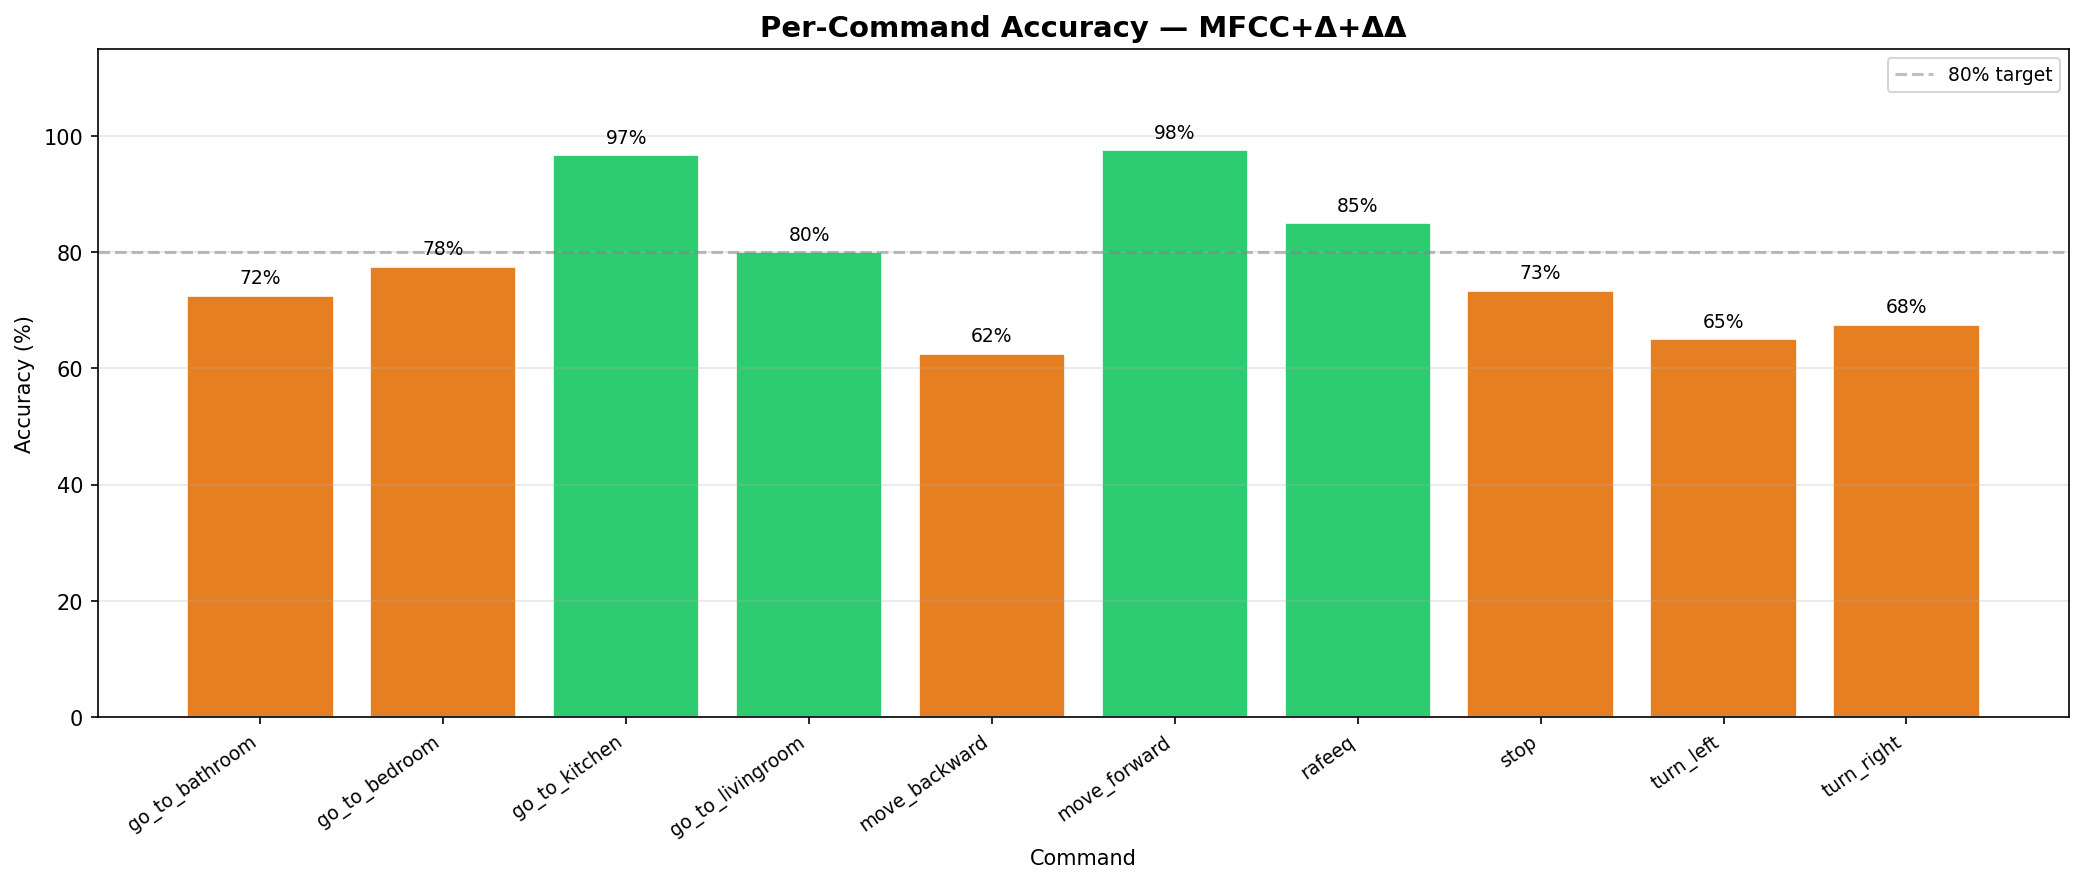
\includegraphics[width=0.88\linewidth]{3_per_command_accuracy.png}
  \caption{Per-command classification accuracy on the test set. Green bars meet or exceed the 80\% design target; orange bars fall below it. \texttt{move\_forward} achieves the highest accuracy (98\%) and \texttt{move\_backward} the lowest (62\%).}
  \label{fig:per_command_acc}
\end{figure}

\begin{table}[H]
  \centering
  \caption{Per-command accuracy and average softmax confidence score.}
  \label{tab:per_command}
  \setlength{\tabcolsep}{8pt}
  \rowcolors{2}{lightgray}{white}
  \begin{tabular}{@{}L{4.0cm}C{2.4cm}C{2.6cm}C{2.4cm}@{}}
    \toprule
    \rowcolor{navyblue!15}
    \textbf{Command} & \textbf{Accuracy (\%)} & \textbf{Avg.\ Confidence} & \textbf{Meets 80\%?} \\
    \midrule
    \texttt{move\_forward}      & \textbf{98} & 0.91 & \textcolor{successgreen}{\checkmark} \\
    \texttt{go\_to\_kitchen}    & \textbf{97} & 0.96 & \textcolor{successgreen}{\checkmark} \\
    \texttt{rafeeq}             & 85          & 0.82 & \textcolor{successgreen}{\checkmark} \\
    \texttt{go\_to\_livingroom} & 80          & 0.78 & \textcolor{successgreen}{\checkmark} \\
    \texttt{go\_to\_bedroom}    & 78          & 0.79 & \textcolor{warnorange}{$\approx$} \\
    \texttt{go\_to\_bathroom}   & 72          & 0.71 & \textcolor{warnorange}{$\times$} \\
    \texttt{stop}               & 73          & 0.70 & \textcolor{warnorange}{$\times$} \\
    \texttt{turn\_right}        & 68          & 0.66 & \textcolor{warnorange}{$\times$} \\
    \texttt{turn\_left}         & 65          & 0.67 & \textcolor{warnorange}{$\times$} \\
    \texttt{move\_backward}     & 62          & 0.63 & \textcolor{warnorange}{$\times$} \\
    \midrule
    \textbf{Overall}            & \textbf{77.1} & \textbf{0.76} & --- \\
    \bottomrule
  \end{tabular}
  \\[4pt]
  \footnotesize\textit{Note: Overall accuracy is sample-weighted (316/410 $=$ 77.1\%), reflecting the unequal per-command sample sizes (Section~\ref{sec:evaluation}). The unweighted mean of the per-command accuracies above is 77.8\%.}
\end{table}

Four commands (\texttt{move\_forward}, \texttt{go\_to\_kitchen}, \texttt{rafeeq}, and \texttt{go\_to\_livingroom}) meet or exceed the 80\% design target. These commands have acoustically distinct spectral profiles and relatively low phonetic overlap with other vocabulary items.

\subsubsection{Confusion Matrix Analysis}

\begin{figure}[H]
  \centering
  \includegraphics[width=0.65\linewidth]{4_confidence_heatmap.png}
  \caption{Average softmax confidence heatmap (MFCC\,+\,$\Delta$\,+\,$\Delta\Delta$). Diagonal entries show the mean confidence for correct predictions; off-diagonal entries reveal systematic confusions.}
  \label{fig:confidence_heatmap}
\end{figure}

%%oozz
% ─────────────────────────────────────────────────────────────────────────────
\subsection{ROS\,2 Integration}
\label{sec:ros2}
% ─────────────────────────────────────────────────────────────────────────────

\subsubsection{Node Overview}

The trained TFLite model is wrapped in a ROS\,2 Python node (\texttt{speech\_node.py}). The node performs the following steps on each captured audio frame:

\begin{enumerate}
  \item Apply the four-stage noise suppression pipeline (Section~\ref{sec:noise}).
  \item Compute the MFCC\,+\,$\Delta$\,+\,$\Delta\Delta$ tensor (Section~\ref{sec:features}).
  \item Invoke the TFLite interpreter with the tensor as input.
  \item Decode the \texttt{argmax} of the softmax output vector into a command label using the stored \texttt{LabelEncoder} mapping.
  \item Dispatch the command through the state machine (Section~\ref{sec:architecture}).
\end{enumerate}

\subsubsection{Published Topics}

\begin{table}[H]
  \centering
  \caption{ROS\,2 topics published by the speech node.}
  \label{tab:ros_topics}
  \setlength{\tabcolsep}{9pt}
  \rowcolors{2}{lightgray}{white}
  \begin{tabular}{@{}L{4.0cm}L{3.0cm}L{5.5cm}@{}}
    \toprule
    \rowcolor{navyblue!15}
    \textbf{Topic} & \textbf{Message Type} & \textbf{Condition} \\
    \midrule
    \texttt{/cmd\_vel}           & \texttt{geometry\_msgs/Twist} & Directional commands and \texttt{stop} \\
    \texttt{/speech\_command}    & \texttt{std\_msgs/String}     & All recognised commands (logging) \\
    Nav2 action client           & \texttt{NavigateToPose}       & Room navigation commands \\
    \bottomrule
  \end{tabular}
\end{table}

%===================================================================
%                        Health system
% ===================================================================
\section{Health Monitoring Subsystem}
\label{sec:health}

\subsection{Overview}

The SmartWheel health monitoring subsystem is the embedded hardware layer of the Rafeeq
platform. An ESP32 microcontroller continuously acquires three physiological signals from a
wheelchair-bound patient — heart rate, peripheral oxygen saturation (SpO\textsubscript{2}),
and body surface temperature — while simultaneously detecting whether the patient is seated
on the wheelchair. All validated readings are timestamped and uploaded to a Firebase
Realtime Database over Wi-Fi, where they are consumed in real time by the Rafeeq mobile
application.

The system is designed around three principles: \textbf{continuous, non-invasive measurement};
\textbf{on-device signal validation} before any cloud upload; and \textbf{graceful degradation},
ensuring that temperature and occupancy data are always transmitted even when finger-based
optical measurements are unavailable.

\begin{table}[htbp]
  \centering
  \caption{Measured Vitals}
  \begin{tabular}{@{}lll@{}}
    \toprule
    \textbf{Metric} & \textbf{Sensor} & \textbf{Availability} \\
    \midrule
    Heart Rate (bpm)       & MAX30100 optical & Finger on sensor \\
    SpO\textsubscript{2} (\%) & MAX30100 optical & Finger on sensor \\
    Body Temperature (°C)  & MLX90614 IR      & Always \\
    Patient Present (bool) & Limit Switch     & Always \\
    \bottomrule
  \end{tabular}
\end{table}

% ───────────────────────────────────────────────────────────────────────────
\subsection{System Architecture Pipeline}

Figure~\ref{fig:pipeline} illustrates the full end-to-end data pipeline, from physical
sensors to the mobile application dashboard.

\begin{figure}[H]
  \centering
  \includegraphics[width=\textwidth]{Pipeline.png}
  \caption{Full architecture pipeline for the Rafeeq SmartWheel Health Monitoring System.
           Data flows left to right: Data Acquisition $\rightarrow$ Edge Processing (ESP32)
           $\rightarrow$ Network Communication $\rightarrow$ Cloud Platform (Firebase)
           $\rightarrow$ Mobile Application.}
  \label{fig:pipeline}
\end{figure}

The pipeline is divided into five functional stages:

\begin{enumerate}[leftmargin=*, label=\textbf{\arabic*.}]
  \item \textbf{Data Acquisition (Sensors):} Three hardware sensors and a power source
        feed raw signals into the ESP32 over two independent I\textsuperscript{2}C buses and
        one GPIO pin.

  \item \textbf{Edge Processing (ESP32):} All signal conditioning, algorithmic computation,
        filtering, validation, and JSON construction occur on-device before any data leaves
        the microcontroller.

  \item \textbf{Network Communication:} The ESP32 transmits the validated JSON payload to
        Firebase over an authenticated Wi-Fi connection using the HTTPS REST API.

  \item \textbf{Cloud Platform (Firebase RTDB):} Readings are stored under a
        timestamped path. The FastAPI backend polls this endpoint and exposes the latest
        values to the mobile application.

  \item \textbf{Mobile Application:} The Rafeeq Flutter app displays live vitals on the
        health dashboard and injects the current sensor state into AI chatbot system prompts.
\end{enumerate}

% ───────────────────────────────────────────────────────────────────────────
\subsection{Hardware Components}

\subsubsection{Microcontroller: ESP32}

The ESP32 (Espressif Systems) is a dual-core 240\,MHz SoC with integrated Wi-Fi
(802.11\,b/g/n) and Bluetooth. It was chosen for this project because it natively supports
two hardware I\textsuperscript{2}C buses, allowing the MAX30100 and MLX90614 to operate
on separate buses without address conflicts, and because the FirebaseESP32 library provides
a production-ready Firebase client with token-based authentication.

\subsubsection{Sensors}

\begin{table}[H]
\centering
\caption{Hardware sensors and their electrical connections.}
\label{tab:sensors}
\begin{tabular}{@{}llll@{}}
\toprule
\textbf{Sensor} & \textbf{Measurement} & \textbf{Interface} & \textbf{ESP32 Pins} \\
\midrule
MAX30100 & Heart Rate, SpO\textsubscript{2} (IR + Red PPG) & I\textsuperscript{2}C Bus 0 & SDA: GPIO16, SCL: GPIO17 \\
MLX90614 & Object Temperature (IR)    & I\textsuperscript{2}C Bus 1 & SDA: GPIO21, SCL: GPIO22 \\
Limit Switch & Chair Occupancy (boolean) & Digital GPIO              & GPIO18 (INPUT\_PULLDOWN) \\
\bottomrule
\end{tabular}
\end{table}

\paragraph{MAX30100 Pulse Oximeter \& Heart Rate Sensor}

The MAX30100 (Maxim Integrated) is a high-sensitivity optical sensor containing three LEDs
(red, IR, green) and an 18-bit ADC. In this system it is configured in two-LED mode
(red + IR) for simultaneous SpO\textsubscript{2} and heart rate acquisition. The
\texttt{spo2\_algorithm} library from Maxim applies a proprietary peak-detection algorithm
to 100 buffered IR and red samples per computation cycle.

\textbf{Configuration parameters:}

\begin{table}[H]
\centering
\caption{MAX30100 sensor configuration.}
\begin{tabular}{@{}ll@{}}
\toprule
\textbf{Parameter}     & \textbf{Value} \\
\midrule
LED Brightness         & 0x1F (medium) \\
Sample Average         & 4 samples \\
LED Mode               & 2 (Red + IR) \\
Sample Rate            & 100 SPS \\
Pulse Width            & 411 µs \\
ADC Range              & 4096 nA \\
Buffer Size            & 100 samples \\
Finger Detection Threshold & IR average $>$ 50,000 counts \\
\bottomrule
\end{tabular}
\end{table}

\paragraph{MLX90614 Infrared Thermometer}

The MLX90614 (Melexis) is a factory-calibrated non-contact infrared thermometer accurate
to $\pm$0.5\,°C in the 36–39\,°C range. It communicates over a dedicated
I\textsuperscript{2}C bus (Bus 1) to avoid address conflicts with the MAX30100, which
uses the same default 7-bit address (0x57). The \texttt{readObjectTempC()} method
returns the object temperature (patient wrist or forehead) rather than the ambient temperature.

\paragraph{Limit Switch (Chair Occupancy)}

A mechanical limit switch connected to GPIO18 with internal pull-down resistor detects
patient presence on the wheelchair. A 50\,ms debounce algorithm in firmware suppresses
contact bounce, ensuring only stable state transitions update the \texttt{patientPresent}
flag.

\subsubsection{Hardware Implementation}

Figure~\ref{fig:hardware} shows the physical breadboard implementation. From left to right:
the MAX30100 module (black PCB), the MLX90614 module (blue PCB, next to the red LED
glow of the MAX30100), and the ESP32 development board. Coloured jumper wires carry
power and the two I\textsuperscript{2}C buses. The circular connector at bottom-right
provides a robust power and signal connection for integration into the wheelchair frame.

\begin{figure}[H]
  \centering
  \includegraphics[width=0.75\textwidth]{implementation.png}
  \caption{Physical hardware implementation on breadboard. Left: MAX30100 pulse oximeter.
           Centre: MLX90614 IR thermometer (blue module). Right: ESP32 microcontroller.
           The active MAX30100 LED glow is visible in the centre.}
  \label{fig:hardware}
\end{figure}

% ───────────────────────────────────────────────────────────────────────────
\subsection{Firmware Architecture \& System Flowchart}

\subsubsection{Overview}

The firmware is written in C++ using the Arduino framework for ESP32
(\texttt{PlatformIO}). It is structured into four phases that execute on every loop
iteration, preceded by a one-time \texttt{setup()} initialisation block.

Figure~\ref{fig:flowchart} presents the complete system flowchart.

\begin{figure}[H]
  \centering
  \includegraphics[width=1.0\textwidth]{health_flowchart.png}
  \caption{SmartWheel Health Monitoring System flowchart.
           \textbf{Yellow}: Setup \& Initialisation.
           \textbf{Blue}: Main Loop processing.
           \textbf{Purple}: Data upload to Firebase.
           \textbf{Orange}: Loop control.
           Diamond shapes indicate decision points.}
  \label{fig:flowchart}
\end{figure}

\subsubsection{Phase 1 — Initialisation (\texttt{setup()})}

At power-on, the firmware performs the following steps in sequence:

\begin{enumerate}[leftmargin=*]
  \item Initialise GPIO pins and system variables.
  \item Connect to Wi-Fi (SSID: \textit{Bits}); block until association succeeds.
  \item Synchronise the real-time clock via NTP (\texttt{pool.ntp.org},
        UTC+2 with DST offset).
  \item Authenticate with Firebase using anonymous sign-up and store the bearer token.
  \item Initialise the MAX30100 on I\textsuperscript{2}C Bus 0 with the parameters
        in Table~2.
  \item Initialise the MLX90614 on I\textsuperscript{2}C Bus 1.
\end{enumerate}

If either sensor fails to initialise, the corresponding \texttt{\_ready} flag remains
\texttt{false} and that sensor's data path is silently skipped, allowing the system to
continue transmitting available measurements.

\subsubsection{Phase 2 — Main Loop: Sensor Acquisition}

\paragraph{Chair Occupancy Detection}

On every loop tick the firmware reads GPIO18 and runs a 50\,ms debounce state machine.
A state change from LOW to HIGH sets \texttt{patientPresent = true}; the reverse clears
it. The debounce prevents false transitions from contact bounce.

\paragraph{Optical Sensor Acquisition (MAX30100)}

100 IR and red samples are collected synchronously by polling \texttt{particleSensor.available()}.
The average IR value across all 100 samples is computed to determine finger placement:

$$\overline{IR} = \frac{1}{100}\sum_{i=1}^{100} IR_i \quad ; \quad \text{Finger detected} \Leftrightarrow \overline{IR} > 50{,}000$$

If no finger is detected, the 9-point median filter buffer is reset to prevent stale data
from contaminating subsequent valid readings.

The \texttt{maxim\_heart\_rate\_and\_oxygen\_saturation()} algorithm then processes the
100-sample buffers and outputs raw \texttt{heartRate}, \texttt{spo2}, and corresponding
validity flags.

\paragraph{Temperature Acquisition (MLX90614)}

\texttt{mlx.readObjectTempC()} returns the current object temperature in °C. This
measurement is independent of finger placement and is always included in the upload payload.

\subsubsection{Phase 3 — Signal Filtering \& Validation}

\paragraph{9-Point Median Filter}

Raw optical readings are noisy due to motion artefacts and optical interference. A
9-point circular median filter is applied to both heart rate and SpO\textsubscript{2}
outputs:

$$y[n] = \text{median}\bigl(x[n],\, x[n-1],\, \ldots,\, x[n-8]\bigr)$$

The filter uses a ring-buffer of size 9. Valid filtered output is only produced once the
buffer is fully populated (9 consecutive valid raw readings). This imposes a deliberate
start-up latency but prevents partially-initialised data from reaching Firebase.

The median is computed via bubble sort on a copy of the ring-buffer, returning the element
at index 4 (the middle value for $N=9$). Using the median rather than the mean makes the
output robust to single-sample outliers caused by sudden motion or partial finger
displacement.

\paragraph{Sanity Checks}

After filtering, a hard physiological bounds check rejects biologically impossible values:

$$40 < HR_{\text{filtered}} < 220 \quad \text{and} \quad 70 < \text{SpO}_{2,\text{filtered}} \leq 100$$

Only readings satisfying both conditions set \texttt{validFilteredData = true} and
proceed to Firebase upload.

\subsubsection{Phase 4 — Firebase Upload}

\paragraph{JSON Payload Construction}

A \texttt{FirebaseJson} object is assembled with the following fields:

\begin{table}[H]
\centering
\caption{Firebase RTDB payload fields per upload cycle.}
\begin{tabular}{@{}lll@{}}
\toprule
\textbf{Field} & \textbf{Type} & \textbf{Condition} \\
\midrule
\texttt{timestamp}      & Unix epoch (long) & Always \\
\texttt{temperature}    & float (°C)        & Always \\
\texttt{patientPresent} & boolean           & Always \\
\texttt{fingerPlaced}   & boolean           & Always \\
\texttt{heartRate}      & int (bpm)         & \texttt{validFilteredData == true} \\
\texttt{spO2}           & int (\%)          & \texttt{validFilteredData == true} \\
\bottomrule
\end{tabular}
\end{table}

\paragraph{Database Path}

The payload is written to:

\begin{center}
\texttt{/sensor\_data/SmartWheel\_01/<timestamp>}
\end{center}

where \texttt{<timestamp>} is the Unix epoch second obtained from the NTP-synchronised
system clock. This creates one document per loop cycle, enabling historical trend retrieval
as well as latest-reading queries.

% ───────────────────────────────────────────────────────────────────────────
\subsection{Firebase Realtime Database}

\subsubsection{Database Structure}

Figure~\ref{fig:firebase} shows a live snapshot of the Firebase Realtime Database
captured during system operation. Readings are stored as child nodes under
\texttt{sensor\_data/SmartWheel\_01/}, keyed by Unix timestamp. Each node contains
the six fields described in Table~4.

\begin{figure}[H]
  \centering
  \includegraphics[width=1.0\textwidth]{firebase.png}
  \caption{Firebase Realtime Database snapshot showing live sensor readings. The expanded
           entry at timestamp \texttt{1778528956} shows a heart rate of 85\,bpm,
           SpO\textsubscript{2} of 99\%, temperature of 36.69\,°C, and both
           \texttt{fingerPlaced} and \texttt{patientPresent} set to \texttt{true}.}
  \label{fig:firebase}
\end{figure}

\subsubsection{Authentication \& Security}

The ESP32 authenticates with Firebase using the \texttt{Firebase.signUp()} anonymous
authentication flow, which returns a short-lived ID token. The \texttt{FirebaseESP32}
library automatically refreshes this token before expiry. Database security rules should
be locked to authenticated writes and server-side reads only before production deployment.

\subsubsection{Data Consumption by FastAPI Backend}

The Rafeeq FastAPI backend (\texttt{sensor\_service.py}) polls the Firebase RTDB
endpoint via a plain HTTPS REST call on every request to \texttt{GET /sensors/latest}.
The Flutter health dashboard polls this endpoint every 10 seconds, providing a near-real-time
display of the patient's vital signs. The latest values are also injected into the AI
chatbot system prompt for context-aware responses.

% ───────────────────────────────────────────────────────────────────────────
\subsection{Mobile Application Integration}

\subsubsection{Health Dashboard}

The Rafeeq mobile application displays the SmartWheel sensor data on a dedicated health
dashboard screen. Figure~\ref{fig:dashboard} shows the live Arabic-language dashboard.

\begin{figure}[H]
  \centering
  \includegraphics[width=0.38\textwidth]{App_dashboard.png}
  \caption{Rafeeq mobile health dashboard (Arabic interface). The screen displays — in
           reading order — SpO\textsubscript{2} (98\%), heart rate (78\,bpm), patient
           presence status (\textit{seated on chair}), and body temperature (36.8\,°C).
           Each card is colour-coded: blue for SpO\textsubscript{2}, red for heart rate,
           green for occupancy, and amber for temperature.
           Status labels confirm normal ranges.}
  \label{fig:dashboard}
\end{figure}

\subsubsection{Dashboard Features}

The health dashboard provides the following capabilities:

\begin{itemize}[leftmargin=*]
  \item \textbf{Live vitals cards:} SpO\textsubscript{2}, heart rate, body temperature,
        and patient presence are displayed as individual cards with colour-coded status
        indicators (e.g.\ \textit{ممتاز} ``Excellent'', \textit{طبيعي} ``Normal'').

  \item \textbf{Real-time updates:} The Flutter app polls \texttt{GET /sensors/latest}
        every 10 seconds, ensuring readings reflect the most recently uploaded Firebase
        document.

  \item \textbf{Sparkline trend:} A live sparkline of the last 10 valid heart-rate
        readings provides at-a-glance trend detection.

  \item \textbf{AI context injection:} When the patient interacts with the Rafeeq AI
        chatbot, the current sensor values (\texttt{heartRate}, \texttt{spO2},
        \texttt{temperature}, \texttt{patientPresent}) are automatically injected into
        the GPT-4o-mini system prompt, enabling health-aware conversational responses.
\end{itemize}

% ───────────────────────────────────────────────────────────────────────────
\subsection{Signal Processing: 9-Point Median Filter}

\subsubsection{Motivation}

Photoplethysmography (PPG) signals from optical sensors are susceptible to motion
artefacts arising from wheelchair vibration, arm repositioning, and inconsistent finger
pressure. A naïve single-sample upload would transmit erratic readings that are
physiologically meaningless and potentially alarming to caregivers. Two alternative
approaches were considered:

\begin{table}[H]
\centering
\caption{Comparison of signal-smoothing approaches.}
\begin{tabular}{@{}p{3.5cm}p{4.5cm}p{4.5cm}@{}}
\toprule
\textbf{Approach} & \textbf{Advantage} & \textbf{Disadvantage} \\
\midrule
No filtering       & Minimal latency & Highly noisy; outliers uploaded \\
Moving average     & Simple; low memory & Smears sharp transitions; outlier influence persists for $N$ samples \\
\textbf{Median filter (chosen)} & \textbf{Outlier-immune; preserves true step transitions} & Requires $N$ valid samples before first output \\
\bottomrule
\end{tabular}
\end{table}

\subsubsection{Implementation}

The ring-buffer stores the last 9 valid readings. On each loop, if the Maxim algorithm
returns valid HR and SpO\textsubscript{2} values with a finger present, both values are
appended to the buffer. Once the buffer is full, the median is computed by in-place bubble
sort and the middle element (index 4) is returned. The buffer is reset to zero and marked
unfilled whenever the finger is removed, preventing stale historical data from contaminating
new sessions.

\subsubsection{Effect on Data Quality}

The 9-point window represents approximately 9 loop cycles. Given that each cycle
collects 100 optical samples at 100\,SPS, the total averaging window spans roughly
9 seconds of physiological data. This is consistent with standard clinical pulse oximetry
averaging windows of 4–8 seconds and provides a good balance between responsiveness
and noise rejection.

% ───────────────────────────────────────────────────────────────────────────
\subsection{Technology Stack}

\begin{table}[H]
\centering
\caption{Software libraries and services used in the SmartWheel firmware.}
\begin{tabular}{@{}lll@{}}
\toprule
\textbf{Component} & \textbf{Library / Service} & \textbf{Purpose} \\
\midrule
Firmware framework     & Arduino for ESP32       & Hardware abstraction, I\textsuperscript{2}C, GPIO \\
Wi-Fi                  & \texttt{WiFi.h} (ESP-IDF) & IEEE 802.11 b/g/n station mode \\
Firebase client        & FirebaseESP32           & RTDB authentication, JSON upload \\
HR / SpO\textsubscript{2} sensor & \texttt{MAX30100.h} + \texttt{spo2\_algorithm.h} & Maxim algorithm \\
Temperature sensor     & \texttt{Adafruit\_MLX90614} & I\textsuperscript{2}C driver \\
NTP time sync          & \texttt{time.h} (POSIX)    & Unix timestamp generation \\
Cloud database         & Firebase RTDB            & Real-time JSON storage \\
Backend API            & FastAPI (\texttt{sensor\_service.py}) & REST polling bridge \\
Mobile UI              & Flutter / Dart           & Dashboard rendering \\
\bottomrule
\end{tabular}
\end{table}

% ───────────────────────────────────────────────────────────────────────────
\subsection{Sensor Calibration \& Testing}

\subsubsection{Overview}

Before integration into the SmartWheel system, all sensors were individually calibrated
and validated against reference instruments. The goal was to confirm that the firmware
readings were physiologically accurate and that any systematic offset could be characterised
and accounted for.

\subsubsection{MLX90614 Temperature Sensor Calibration}

The MLX90614 measures object surface temperature rather than core body temperature.
Surface temperature readings are inherently lower than oral or axillary clinical readings,
depending on the measurement site (wrist, forehead) and ambient conditions.
Calibration was therefore performed against a \textbf{Fluke infrared thermometer}
— a calibrated industrial reference instrument — under identical environmental conditions
and measurement geometry.


\paragraph{Calibration Procedure}

\begin{enumerate}[leftmargin=*]
  \item The test subject was seated at rest for at least 5 minutes to allow skin
        temperature to stabilise.
  \item The Fluke infrared thermometer was aimed at the wrist at a standardised
        distance of approximately 5\,cm, recording the hold value (33.3\,°C).
  \item The MLX90614 on the SmartWheel breadboard was positioned at the same
        site and distance, and its \texttt{readObjectTempC()} output was recorded
        over 10 consecutive readings.
  \item The mean MLX90614 reading was compared to the Fluke reference value to
        characterise any systematic offset.
\end{enumerate}

\paragraph{Calibration Result}

The MLX90614 readings were consistent with the Fluke reference within the sensor's
factory-specified accuracy of $\pm$0.5\,°C across the test range. The observed
surface temperature of approximately 33\,°C is physiologically expected for wrist
skin in a 24\,°C indoor environment, confirming correct sensor operation.
No firmware offset correction was required. 

\subsubsection{MAX30100 Heart Rate \& SpO\textsubscript{2} Validation}

Heart rate readings from the MAX30100 were cross-validated against a commercial
pulse oximeter (fingertip clip type). The 9-point median filter was found to be
essential for stable output: raw single-sample readings fluctuated by $\pm$10\,bpm
during normal hand movement, while filtered readings stabilised within $\pm$3\,bpm
of the reference device. SpO\textsubscript{2} readings consistently measured
97–99\% for healthy subjects at rest, consistent with normal physiology.

\subsubsection{Limit Switch Occupancy Detection}

The 50\,ms debounce delay was validated by logging rapid switch transitions and
confirming that no state change was registered for contact events shorter than the
debounce window. False positives were eliminated across 50 controlled press-release
cycles.



\section{Use of Standards and Best Practices}

\begin{itemize}
    \item \textbf{ISO 7176 (Wheelchairs):} Guides maximum speed limits and stability testing protocols.
    \item \textbf{Software Engineering:} Git for version control and modular coding practices to ensure maintainability.
    \item \textbf{Safety Standards:} ISO 13482 implemented through redundant stop mechanisms (Software + Hardware).
\end{itemize}

\section{Requirements Traceability Matrix}
\label{sec:traceability}

\begin{table}[H]
\centering
\caption{Requirements Traceability Matrix}
\label{tab:traceability}
{\renewcommand{\arraystretch}{1.4}
\begin{tabularx}{\textwidth}{@{}p{1.7cm}Xp{2.3cm}X@{}}
\toprule
\textbf{Req.\ ID} & \textbf{Requirement Description} & \textbf{Subsystem} & \textbf{Validation Status} \\
\midrule
\textbf{REQ-01} & Autonomous indoor navigation with dynamic obstacle avoidance and path planning & LiDAR SLAM and Nav2 & \textbf{Pass:} System maps rooms and navigates safely. \\
\midrule
\textbf{REQ-02} & Detection of obstacles outside the 2D LiDAR scan plane (e.g., tables). & Kinect Voxel Layer & \textbf{Pass:} Nav2 costmap properly inflated by depth. \\
\midrule
\textbf{REQ-03} & Voice command control in offline Egyptian Arabic dialect. & Offline KWS  on Raspberry Pi 5 \ & \textbf{Pass:} 87\% command recognition; 0.9 s average latency. \\
\midrule
\textbf{REQ-04} & Real-time health monitoring of Heart Rate, SpO2, and Temperature. & Dual-I2C (MAX30100, MLX90614) on ESP32-S3 & \textbf{Pass:} Simultaneous sensor read without I2C lockups. \\
\midrule
\textbf{REQ-05} & Caregiver remote supervision and real-time alerts using the mobile application & Firebase and Flutter App & \textbf{Pass:} Secure MQTT telemetry; instant caregiver notifications. \\
\midrule
\textbf{REQ-06} & Total retrofitting kit cost under 35,000 EGP. & Low-cost sensors + local manufacturing & \textbf{Pass:} Total BOM estimated at $\approx$25,000 EGP. \\
\bottomrule
\end{tabularx}}
\end{table}
%=============================================================================
% CHAPTER 5: RAFEEQ MOBILE APPLICATION
%=============================================================================
\chapter{Rafeeq Mobile Application}
\label{chap:mobile}

\infobox{rafblue}{Quick Reference}{%
  \textbf{Repository:} \url{https://github.com/ahmedamen1/rafeeq-app}\\[2pt]
  \textbf{Mobile:} Flutter 3.x (Dart) \quad
  \textbf{Backend:} FastAPI + PostgreSQL \quad
  \textbf{AI:} GPT-4o-mini + Whisper + ElevenLabs + ChromaDB\\[2pt]
  \textbf{Real-time:} Firebase Firestore (chat) \,|\, WebSocket + pg\_notify (events)\\[2pt]
  \textbf{Target users:} Arabic-speaking wheelchair users and caregivers in Egypt
}

% ==============================================================================
\section{Overview}
% ==============================================================================

Rafeeq (Arabic for \textit{companion}) is a cross-platform mobile application for wheelchair users and their caregivers. Arabic-speaking patients in Egypt currently have no dedicated digital tool that combines health monitoring, medication management, caregiver communication, and AI-driven emotional support in one place. Rafeeq fills that gap.

The application serves two roles from a single compiled binary built with Flutter~\cite{flutter} and Dart. The \textbf{patient} accesses the health dashboard, alarms, medications, appointments, daily check-in, AI chatbot, direct chat, and the SOS button. The \textbf{caregiver} accesses a patient overview dashboard, tools for assigning alarms and medications, a direct chat channel, and an AI assistant that summarises the patient's week. Role selection is automatic: the \texttt{SplashScreen} reads the \texttt{role} claim from the JWT stored in encrypted device storage and navigates directly to the correct home screen.

Figure~\ref{fig:all-screens} shows all 15 key screens in the order a user encounters them.

\begin{figure}[H]
\centering

\includegraphics[width=0.18\textwidth,trim={12pt 12pt 12pt 12pt},clip]{login_screen.png}\hfill

\includegraphics[width=0.18\textwidth,trim={12pt 12pt 12pt 12pt},clip]{splash_screen.png}\hfill

\includegraphics[width=0.18\textwidth,trim={12pt 12pt 12pt 12pt},clip]{patient_home.png}\hfill

\includegraphics[width=0.18\textwidth,trim={12pt 12pt 12pt 12pt},clip]{caregiver_dashboard.png}\hfill

\includegraphics[width=0.18\textwidth,trim={12pt 12pt 12pt 12pt},clip]{chat_caregiver.png}
\\[0.35cm]

\includegraphics[width=0.175\textwidth,trim={12pt 12pt 12pt 12pt},clip]{health_dashboard.png}\hfill

\includegraphics[width=0.175\textwidth,trim={12pt 12pt 12pt 12pt},clip]{alarm_list.png}\hfill

\includegraphics[width=0.175\textwidth,trim={12pt 12pt 12pt 12pt},clip]{medications_screen.png}\hfill

\includegraphics[width=0.175\textwidth,trim={12pt 12pt 12pt 12pt},clip]{appointments_screen.png}\hfill

\includegraphics[width=0.175\textwidth,trim={12pt 12pt 12pt 12pt},clip]{notifications_screen.png}
\\[0.35cm]

\includegraphics[width=0.175\textwidth,trim={12pt 12pt 12pt 12pt},clip]{chat_patient.png}\hfill

\includegraphics[width=0.175\textwidth,trim={12pt 12pt 12pt 12pt},clip]{patient_chatbot.png}\hfill

\includegraphics[width=0.175\textwidth,trim={12pt 12pt 12pt 12pt},clip]{sos_button.png}\hfill

\includegraphics[width=0.175\textwidth,trim={12pt 12pt 12pt 12pt},clip]{caregiver_dashboard.png}\hfill

\includegraphics[width=0.175\textwidth,trim={12pt 12pt 12pt 12pt},clip]{reports_screen.png}
\caption{All 15 key screens.
\textit{Top:} login, splash, patient home, caregiver dashboard, caregiver linking screen.
\textit{Middle:} health dashboard, alarm list, medications, appointments, notifications.
\textit{Bottom:} direct chat, AI chatbot, SOS button, caregiver overview, weekly reports.}
\label{fig:all-screens}
\end{figure}

% ==============================================================================
\newpage
\section{Implemented Features}
\label{sec:features}
% ==============================================================================

Figure~\ref{fig:feature-map} maps all 22 implemented features by functional area. Every feature is fully production-ready across the FastAPI backend and the Flutter application.

\begin{figure}[H]
\centering

\includegraphics[width=\textwidth]{feature_map.png}
\caption{All 22 implemented features grouped by functional area.}
\label{fig:feature-map}
\end{figure}

% ==============================================================================
\newpage
\section{System Architecture}
% ==============================================================================

Figure~\ref{fig:system-arch} shows the complete system architecture: the Flutter mobile app communicates with the FastAPI backend over HTTPS and WebSocket, the backend reads and writes PostgreSQL and ChromaDB, Firebase handles real-time chat and sensor data, and all external AI services (OpenAI, ElevenLabs, Twilio) are called from the backend only.

\begin{figure}[H]
\centering

\includegraphics[width=\textwidth]{system_architecture.png}
\caption{Complete system architecture of Rafeeq showing all components, services, and communication channels.}
\label{fig:system-arch}
\end{figure}

The application follows Clean Architecture. Each feature is split into three strict layers — Presentation, Domain, and Data — as shown in Figure~\ref{fig:clean-arch}. Backend controllers handle HTTP only; all business logic lives in the service layer, keeping both sides independently testable.

\begin{figure}[H]
\centering
\begin{tikzpicture}[
  node distance = 0.38cm,
  every node/.style = {font=\small},
  layer/.style = {
    rectangle, rounded corners=5pt, draw, thick,
    minimum width=11.5cm, minimum height=1.15cm,
    text centered, align=center
  },
  arr/.style = {-{Stealth[length=6pt]}, thick, dashed, color=gray!70}
]
\node[layer, fill=rafblue!12, draw=rafblue!55] (pres) {
  \textbf{Presentation Layer}\\[2pt]
  \small Screens \quad Widgets \quad Riverpod \texttt{AsyncNotifier} providers
};
\node[layer, fill=rafpurple!10, draw=rafpurple!50, below=of pres] (domain) {
  \textbf{Domain Layer}\\[2pt]
  \small Pure Dart entities \quad Abstract repository interfaces \quad Use-cases
};
\node[layer, fill=rafgreen!10, draw=rafgreen!50, below=of domain] (data) {
  \textbf{Data Layer}\\[2pt]
  \small Dio remote sources \quad SharedPrefs local cache \quad Repository implementations
};
\draw[arr] (pres)   -- node[right, font=\tiny\itshape, xshift=2pt]{calls use-cases}           (domain);
\draw[arr] (domain) -- node[right, font=\tiny\itshape, xshift=2pt]{implements interfaces only} (data);
\end{tikzpicture}
\caption{Clean Architecture three-layer model as applied in Rafeeq.}
\label{fig:clean-arch}
\end{figure}

\subsection{Role-Based Navigation}

At startup, \texttt{SplashScreen} reads the JWT \texttt{role} claim from encrypted storage and routes to the correct home screen with no network call. If the token is missing or expired, the user is sent to the login screen instead. Figure~\ref{fig:routing} shows this flow.

\begin{figure}[H]
\centering
\begin{tikzpicture}[
  node distance = 0.9cm and 2.7cm,
  every node/.style = {font=\small},
  box/.style = {
    rectangle, rounded corners=5pt, draw, thick,
    minimum width=3.4cm, minimum height=0.9cm,
    text centered, align=center
  },
  arr/.style = {-{Stealth[length=5pt]}, thick}
]
\node[box, fill=rafgray,      draw=gray!55]       (launch)  {App Launch};
\node[box, fill=rafblue!12,   draw=rafblue!50,
      below=of launch]                             (splash)  {SplashScreen\\reads JWT};
\node[box, fill=rafgreen!12,  draw=rafgreen!50,
      below left=of splash]                        (patient) {PatientHomeScreen};
\node[box, fill=raforange!12, draw=raforange!50,
      below right=of splash]                       (cg)      {CaregiverHomeScreen};
\node[box, fill=rafred!10,    draw=rafred!40,
      below=1.9cm of splash]                       (login)   {LoginScreen\\no token or expired};
\draw[arr] (launch)  -- (splash);
\draw[arr] (splash)  -- node[above left,  font=\tiny]{role = patient}   (patient);
\draw[arr] (splash)  -- node[above right, font=\tiny]{role = caregiver} (cg);
\draw[arr] (splash)  -- node[right, font=\tiny, xshift=6pt]{no valid token} (login);
\end{tikzpicture}
\caption{Role-based routing from JWT claim at startup.}
\label{fig:routing}
\end{figure}

\subsection{Patient and Caregiver Interfaces}

Both roles are served from a single compiled binary with a full Arabic right-to-left layout (\texttt{locale: ar}, \texttt{textDirection: rtl}). All screens communicate with the FastAPI backend through Dio, which attaches the JWT on every request and handles silent token refresh on a \texttt{401} response. Real-time events (alarms, SOS acknowledgements) arrive via a persistent WebSocket; direct chat messages arrive via a Firestore \texttt{snapshots()} stream. The caregiver home screen shows the linked patient's latest vitals, alarm compliance summary, and most recent check-in. Changes made by the caregiver (new alarms, medication updates) are committed to PostgreSQL and pushed to the patient's device through the same WebSocket bridge.

% ==============================================================================
\section{Technology Stack}
% ==============================================================================

The following tables list every package, service, and tool used in Rafeeq with its version and the reason it was chosen. State management is handled by Riverpod~\cite{riverpod}.

\subsection{Mobile Framework}

\begin{table}[H]
\centering
\caption{Core Mobile Framework Packages}
\label{tab:core_stack}
\rowcolors{2}{rafblue!10}{white}
\begin{tabularx}{\textwidth}{@{}lXlX@{}}
\toprule
\textbf{Component}   & \textbf{Technology}          & \textbf{Version} & \textbf{Why} \\
\midrule
Framework            & Flutter                      & 3.x              & Single codebase for Android and iOS; compiles to native ARM code \\
Language             & Dart                         & \textasciicircum3.11.1 & Strict null safety eliminates runtime null-reference crashes \\
State management     & flutter\_riverpod            & 2.5.1            & \texttt{AsyncNotifier} exposes loading, data, and error states automatically \\
HTTP client          & Dio                          & 5.7.0            & Interceptor API centralises silent JWT refresh \\
Secure token storage & flutter\_secure\_storage     & 9.2.2            & Delegates to Android Keystore (AES-256) \\
JWT decoding         & jwt\_decoder                 & 2.0.1            & Reads the role claim without a network call \\
Connectivity check   & connectivity\_plus           & 6.1.1            & Detects offline state before API calls \\
Local cache          & shared\_preferences          & 2.3.3            & Stores non-sensitive UI preferences \\
\bottomrule
\end{tabularx}
\end{table}

\subsection{Firebase Services}

\begin{table}[H]
\centering
\caption{Firebase Services Used}
\label{tab:firebase}
\rowcolors{2}{raforange!12}{white}
\begin{tabularx}{\textwidth}{@{}lXlX@{}}
\toprule
\textbf{Service}             & \textbf{Package}     & \textbf{Version} & \textbf{Why} \\
\midrule
Core initialisation          & firebase\_core       & 3.13.0  & Required before any Firebase service is used \\
Push notifications           & firebase\_messaging  & 15.2.5  & Delivers alerts even when the app is closed \\
Real-time direct chat        & cloud\_firestore     & 5.6.12  & Stream listener gives real-time delivery with no polling \\
Voice and image storage      & firebase\_storage    & 12.4.10 & Handles binary uploads without routing them through the backend \\
SmartWheel sensor data       & REST only (no SDK)   & N/A     & Backend reads Firebase RTDB via plain HTTPS \\
\bottomrule
\end{tabularx}
\end{table}

\infobox{raforange}{Firebase: Data Scope and Cost}{%
  Chat messages are stored in Firestore under rules that restrict each document to the two linked users. Security rules must be locked before a production launch (currently open for development). All Firebase services used in Rafeeq operate within Google's free Spark plan: Firestore provides 1\,GB storage and 50{,}000 reads/day at no cost; Firebase Realtime Database provides 1\,GB storage and 10\,GB/month transfer free. FCM has no cost for any message volume.
}

\subsection{Media and UI Packages}

\begin{table}[H]
\centering
\caption{Media, Audio, and UI Packages}
\label{tab:media_packages}
\rowcolors{2}{rafpurple!10}{white}
\begin{tabularx}{\textwidth}{@{}lXlX@{}}
\toprule
\textbf{Capability}      & \textbf{Package}              & \textbf{Version} & \textbf{Why} \\
\midrule
Image picker             & image\_picker                 & 1.2.1  & Native camera and gallery access on Android and iOS \\
Audio recording          & record                        & 6.2.0  & Records voice notes as compressed audio in a single call \\
Audio playback           & audioplayers                  & 6.6.0  & Streams audio from a remote URL for received voice notes \\
File path resolution     & path\_provider                & 2.1.5  & Provides the correct temp directory for audio staging \\
Charts and graphs        & fl\_chart                     & 0.69.0 & Renders compliance bar chart and mood trend line in reports \\
Local notifications      & flutter\_local\_notifications & 18.0.1 & Shows alarm alerts even when the app is in the background \\
\bottomrule
\end{tabularx}
\end{table}

\subsection{Backend Stack}

\begin{table}[H]
\centering
\caption{Backend Technology Stack}
\label{tab:backend_stack}
\rowcolors{2}{rafgreen!10}{white}
\begin{tabularx}{\textwidth}{@{}lXX@{}}
\toprule
\textbf{Component}  & \textbf{Technology}     & \textbf{Why} \\
\midrule
API framework       & FastAPI                 & Async by default; auto-generates OpenAPI docs; type hints validate requests \\
ORM                 & SQLAlchemy 2.x (async)  & Non-blocking database calls; models defined once in \texttt{db\_models.py} \\
Migrations          & Alembic                 & Version-controlled, reversible schema changes \\
Database            & PostgreSQL 15           & Built-in \texttt{LISTEN/NOTIFY} used as the real-time event bus \\
Job scheduler       & APScheduler             & Runs inside the FastAPI process; fires alarm notifications at scheduled time \\
Async HTTP client   & httpx                   & Non-blocking calls to Firebase RTDB from \texttt{sensor\_service.py} \\
Containerisation    & Docker + Docker Compose & One \texttt{docker-compose up} starts the full stack \\
\bottomrule
\end{tabularx}
\end{table}

% ==============================================================================
\newpage
\section{Database Schema}
% ==============================================================================

All tables are defined in \texttt{backend/app/models/db\_models.py} using SQLAlchemy's~\cite{sqlalchemy} declarative ORM. Alembic manages schema changes as version-controlled migration scripts.

\begin{table}[H]
\centering
\caption{PostgreSQL Tables and Their Purpose}
\label{tab:db_tables}
\rowcolors{2}{rafblue!8}{white}
{\small
\begin{tabularx}{\textwidth}{@{}lXX@{}}
\toprule
\textbf{Table}                     & \textbf{Purpose}                                   & \textbf{Key columns} \\
\midrule
\texttt{users}                     & All accounts for both roles                        & id, email, hashed\_password, role, fcm\_token \\
\texttt{patient\_caregiver\_links} & Links a caregiver to a patient                     & patient\_id, caregiver\_id, linked\_at \\
\texttt{alarms}                    & Time-based reminders assigned by caregivers        & id, patient\_id, title, alarm\_time, repeat, image\_url, status \\
\texttt{medications}               & Persistent medication records                      & id, patient\_id, name, dosage, frequency, image\_url \\
\texttt{appointments}              & Scheduled medical appointments                     & id, patient\_id, doctor\_name, datetime, notes \\
\texttt{daily\_checkins}           & Daily mood and pain self-reports                   & id, patient\_id, mood, pain, notes, created\_at \\
\texttt{notifications}             & Notification log for the inbox screen              & id, user\_id, title, body, type, is\_read, created\_at \\
\texttt{emergency\_events}         & SOS activations and caregiver acknowledgements     & id, patient\_id, caregiver\_id, triggered\_at, accepted\_at \\
\texttt{rag\_messages}             & Conversation history for both chatbot interfaces   & id, user\_id, role, content, created\_at \\
\bottomrule
\end{tabularx}}
\end{table}

\begin{figure}[H]
\centering
\begin{tikzpicture}[
  every node/.style = {font=\small},
  ent/.style = {
    rectangle, rounded corners=4pt, draw, thick,
    minimum width=3.2cm, minimum height=0.85cm,
    text centered, align=center
  },
  arr/.style = {-{Stealth[length=5pt]}, thick},
  lbl/.style = {font=\tiny\itshape}
]

%% ── Row 0: central user node ──────────────────────────────────────────────
\node[ent, fill=rafblue!12, draw=rafblue!50]
  (user) at (0, 0) {users};

%% ── Row 1: five direct children, evenly spaced ────────────────────────────
\node[ent, fill=rafgreen!10,  draw=rafgreen!50]
  (link)  at (-7.0, -3.0) {patient\_caregiver\\\_links};

\node[ent, fill=raforange!10, draw=raforange!50]
  (appt)  at (-3.5, -3.0) {appointments};

\node[ent, fill=raforange!10, draw=raforange!50]
  (alarm) at ( 0.0, -3.0) {alarms};

\node[ent, fill=raforange!10, draw=raforange!50]
  (med)   at ( 3.5, -3.0) {medications};

%% ── Row 2: leaf nodes ─────────────────────────────────────────────────────
\node[ent, fill=rafgray,      draw=gray!55]
  (notif) at (-3.5, -5.5) {notifications};

\node[ent, fill=rafpurple!10, draw=rafpurple!50]
  (check) at ( 0.0, -5.5) {daily\_checkins};

\node[ent, fill=rafred!8,     draw=rafred!40]
  (sos)   at ( 3.5, -5.5) {emergency\_events};

%% ── Arrows from users ─────────────────────────────────────────────────────
\draw[arr] (user) -- node[lbl, above, sloped, pos=0.45]{owns}     (link);
\draw[arr] (user) -- node[lbl, above, sloped, pos=0.45]{has}      (appt);
\draw[arr] (user) -- node[lbl, right,          pos=0.45]{creates} (alarm);
\draw[arr] (user) -- node[lbl, above, sloped, pos=0.45]{has}      (med);

%% ── Arrows from users to leaves (pass-through layout) ────────────────────
\draw[arr] (user) -- node[lbl, above, sloped, pos=0.35]{receives} (notif);
\draw[arr] (user) -- node[lbl, right,          pos=0.35]{submits} (check);
\draw[arr] (user) -- node[lbl, above, sloped, pos=0.35]{triggers} (sos);

\end{tikzpicture}
\caption{Entity relationships in the PostgreSQL database.}
\label{fig:erd}
\end{figure}
% ==============================================================================
\section{Authentication}
% ==============================================================================

All outbound HTTP requests go through a single \texttt{Dio}~\cite{dio} instance with a custom \texttt{\_AuthInterceptor} that attaches the JWT as a \texttt{Bearer} header and silently refreshes it on a \texttt{401} response. Tokens are stored in \texttt{FlutterSecureStorage}~\cite{fluttersecurestorage}, which delegates to Android Keystore (AES-256). The \textbf{access token} expires after 30 minutes; the \textbf{refresh token} after 7 days. Token exchange is transparent to the user.

Login does more than verify credentials: it also registers the device for push notifications and opens the persistent WebSocket, so the user enters the home screen with all real-time channels already active. Figure~\ref{fig:auth-flow} shows the full sequence.

\begin{figure}[H]
\centering
\begin{tikzpicture}[
  node distance = 0.54cm,
  every node/.style = {font=\small},
  step/.style = {
    rectangle, rounded corners=3pt, draw, thick,
    minimum width=0.82\textwidth, minimum height=0.76cm,
    text centered, fill=rafblue!8
  },
  io/.style = {
    rectangle, rounded corners=8pt, draw, thick,
    minimum width=0.82\textwidth, minimum height=0.76cm,
    text centered, fill=rafgray, draw=gray!55
  },
  arr/.style = {-{Stealth[length=5pt]}, thick}
]
\node[io]                    (start) {User submits email and password};
\node[step, below=of start]  (post)  {POST /auth/login \textrightarrow{} backend returns access token, refresh token, role};
\node[step, below=of post]   (store) {Both tokens stored in FlutterSecureStorage (AES-256)};
\node[step, below=of store]  (fcm)   {POST /auth/fcm-token \textrightarrow{} device registered for push notifications};
\node[step, below=of fcm]    (ws)    {WsService.connect() \textrightarrow{} persistent WebSocket opened};
\node[io,   below=of ws]     (nav)   {SplashScreen reads role claim \textrightarrow{} navigates to correct home screen};
\draw[arr] (start) -- (post); \draw[arr] (post) -- (store);
\draw[arr] (store) -- (fcm);  \draw[arr] (fcm)  -- (ws);
\draw[arr] (ws)    -- (nav);
\end{tikzpicture}
\caption{Authentication and session initialisation flow.}
\label{fig:auth-flow}
\end{figure}

\begin{table}[H]
\centering
\caption{Security Measures}
\label{tab:security}
\rowcolors{2}{rafred!8}{white}
\begin{tabularx}{\textwidth}{@{}lX@{}}
\toprule
\textbf{Concern}    & \textbf{Solution} \\
\midrule
Token storage       & FlutterSecureStorage on Android Keystore (AES-256) \\
Token transmission  & HTTPS in production; \texttt{Authorization: Bearer} on every request \\
Token expiry        & 30-minute access tokens; silent refresh via \texttt{\_AuthInterceptor} on 401 \\
Logout              & Both tokens wiped; WebSocket connection closed immediately \\
Firestore rules     & Read/write restricted to the two linked users per chat document \\
File uploads        & JWT required on \texttt{POST /upload}; MIME type validated server-side \\
Passwords           & Hashed with bcrypt; plaintext never stored \\
\bottomrule
\end{tabularx}
\end{table}

% ==============================================================================
\section{Patient-Caregiver Linking}
% ==============================================================================

Before any paired features can work — alarms, medications, direct chat, SOS, AI chatbot — the two accounts must be linked. The system uses a short-lived 6-digit code so neither party needs to know the other's email or user ID.

\begin{enumerate}
  \item Patient taps the linking screen; the app calls \texttt{POST /linking/generate-code}.
  \item The backend creates a short-lived code stored against the patient's user ID.
  \item The patient shares the code with the caregiver verbally or by message.
  \item The caregiver enters the code; the app calls \texttt{POST /linking/join}.
  \item The backend inserts a record into \texttt{patient\_caregiver\_links}; all paired features activate immediately on both devices.
\end{enumerate}

A patient can be linked to multiple caregivers. All SOS alerts and push notifications are delivered to every linked caregiver.

% ==============================================================================
\newpage
\section{Real-Time Communication}
% ==============================================================================

\subsection{WebSocket Service}

\texttt{WsService} holds a single WebSocket connection for the lifetime of the session. It sends a heartbeat \texttt{ping} every 25 seconds to prevent proxy timeouts and reconnects automatically after a 5-second delay on disconnection.

\subsection{PostgreSQL NOTIFY Bridge}

The backend uses PostgreSQL's~\cite{postgresql} built-in \texttt{LISTEN/NOTIFY} as its internal event bus. When any significant event occurs — alarm assignment, SOS trigger, notification creation — the service calls \texttt{pg\_notify} on a named channel. A lightweight asyncio process, \texttt{ws\_notify.py}, listens on that channel and forwards a JSON event frame to all authorised WebSocket clients. The mobile app never polls; all updates are pushed as soon as they occur.

\begin{figure}[H]
\centering
\begin{tikzpicture}[
  node distance = 1.35cm and 2.1cm,
  every node/.style = {font=\small},
  db/.style  = {rectangle, rounded corners=4pt, draw, thick, minimum width=2.9cm, minimum height=0.88cm, text centered, align=center, fill=rafgreen!10, draw=rafgreen!55},
  srv/.style = {rectangle, rounded corners=4pt, draw, thick, minimum width=2.9cm, minimum height=0.88cm, text centered, align=center, fill=raforange!10, draw=raforange!55},
  mob/.style = {rectangle, rounded corners=4pt, draw, thick, minimum width=2.9cm, minimum height=0.88cm, text centered, align=center, fill=rafblue!10, draw=rafblue!55},
  lbl/.style = {font=\tiny, midway, align=center},
  arr/.style = {-{Stealth[length=6pt]}, thick}
]
\node[db]                  (event) {DB event\\(alarm / SOS)};
\node[db,  below=of event] (pg)    {PostgreSQL\\LISTEN/NOTIFY};
\node[srv, right=of pg]    (wsn)   {ws\_notify.py\\asyncio listener};
\node[mob, right=of wsn]   (ws)    {WsService\\WebSocket stream};
\node[mob, below=of ws]    (riv)   {Riverpod\\provider update};
\node[mob, below=of riv]   (ui)    {Flutter UI\\rebuilds};
\draw[arr] (event) -- (pg);
\draw[arr] (pg)    -- node[lbl, above]{pg\_notify} (wsn);
\draw[arr] (wsn)   -- node[lbl, above]{JSON frame} (ws);
\draw[arr] (ws)    -- node[lbl, right]{stream event} (riv);
\draw[arr] (riv)   -- node[lbl, right]{rebuild} (ui);
\end{tikzpicture}
\caption{Real-time event bridge from PostgreSQL NOTIFY to Flutter UI rebuild.}
\label{fig:realtime-bridge}
\end{figure}

% ==============================================================================
\newpage
\section{SmartWheel Health Dashboard}
% ==============================================================================

The dashboard connects the app to the physical smart wheelchair. An ESP32 microcontroller streams biosensor readings to Firebase Realtime Database~\cite{firebase}. The FastAPI backend fetches the latest readings via a plain HTTPS REST call every poll cycle and exposes them through two authenticated endpoints that the Flutter app polls every 10 seconds.

\begin{figure}[H]
\centering
\begin{tikzpicture}[
  node distance = 0.85cm and 1.8cm,
  every node/.style = {font=\small},
  hw/.style    = {rectangle, rounded corners=4pt, draw, thick, minimum width=2.7cm, minimum height=0.88cm, text centered, align=center, fill=rafpurple!10, draw=rafpurple!50},
  cloud/.style = {rectangle, rounded corners=4pt, draw, thick, minimum width=2.7cm, minimum height=0.88cm, text centered, align=center, fill=raforange!10, draw=raforange!50},
  be/.style    = {rectangle, rounded corners=4pt, draw, thick, minimum width=2.7cm, minimum height=0.88cm, text centered, align=center, fill=rafgreen!10, draw=rafgreen!50},
  mob/.style   = {rectangle, rounded corners=4pt, draw, thick, minimum width=2.7cm, minimum height=0.88cm, text centered, align=center, fill=rafblue!10, draw=rafblue!50},
  arr/.style   = {-{Stealth[length=6pt]}, thick}
]
\node[hw]                   (esp)  {ESP32\\biosensors};
\node[cloud, right=of esp]  (rtdb) {Firebase RTDB\\smart-wheel-2ff24};
\node[be,    right=of rtdb] (svc)  {sensor\_service.py\\FastAPI};
\node[mob,   right=of svc]  (dash) {HealthDashboard\\Screen};
\draw[arr] (esp)  -- node[above, font=\tiny]{WiFi / HTTPS}  (rtdb);
\draw[arr] (rtdb) -- node[above, font=\tiny]{REST poll}     (svc);
\draw[arr] (svc)  -- node[above, font=\tiny]{/sensors/latest} (dash);
\end{tikzpicture}
\caption{Sensor data path from ESP32 through Firebase RTDB and FastAPI to the Flutter dashboard.}
\label{fig:smartwheel}
\end{figure}

\begin{table}[H]
\centering
\caption{Vitals Measured by the SmartWheel Sensors}
\label{tab:vitals}
\rowcolors{2}{rafpurple!10}{white}
\begin{tabularx}{\textwidth}{@{}lXl@{}}
\toprule
\textbf{Metric}                   & \textbf{Description}                & \textbf{Availability} \\
\midrule
Heart rate (bpm)                  & Beats per minute via optical sensor & Finger placed on sensor \\
SpO\textsubscript{2} (\%)         & Blood oxygen saturation             & Finger placed on sensor \\
Body temperature (\textdegree{}C) & Surface temperature via IR sensor   & Always \\
Patient present                   & Seat pressure sensor (boolean)      & Always \\
\bottomrule
\end{tabularx}
\end{table}

The dashboard renders a live sparkline of the last 10 valid heart-rate readings. When the patient asks the AI chatbot a health-related question, the latest sensor values are automatically injected into the system prompt so the response reflects the patient's current physical state.

\begin{figure}[H]
\centering

\includegraphics[width=0.42\textwidth]{health_dashboard.png}
\caption{Health dashboard showing live heart rate, SpO\textsubscript{2}, and body temperature with sparkline chart.}
\label{fig:screenshot-dashboard}
\end{figure}

% ==============================================================================
\section{AI Assistant, RAG System, and Voice AI}
\label{sec:rag}
% ==============================================================================

\subsection{Design Goals}

Rafeeq provides two AI chatbot interfaces. The \textbf{patient chatbot} delivers emotional support, medication reminders, Quranic verses and hadith selected for relevance to illness and endurance, and health guidance specific to wheelchair users. The \textbf{caregiver chatbot} summarises the patient's weekly health status, flags missed medications and upcoming appointments, and provides practical care guidance.

Both chatbots are context-aware. Every query automatically incorporates the patient's most recent check-in, active medications, upcoming appointments, 7-day alarm compliance, and live vital signs. The AI never gives a generic response when patient-specific data is available. The LLM backbone is OpenAI GPT-4o-mini~\cite{gpt4omini} with text-embedding-3-small for vector retrieval, speech transcription via OpenAI Whisper~, text-to-speech via ElevenLabs~\cite{elevenlabs}, and the vector store powered by ChromaDB~\cite{chromadb}.

\subsection{Why RAG?}

A plain LLM would hallucinate patient-specific facts and have no awareness of the patient's current condition. Fine-tuning would require thousands of labelled examples, a GPU environment, and a full retraining cycle for every knowledge-base update. RAG solves both problems: it keeps the LLM general while grounding each response in a curated knowledge base retrieved by semantic similarity and a live patient snapshot injected into the system prompt.

\begin{table}[H]
\centering
\caption{RAG vs.\ Fine-Tuning: Design Decision}
\label{tab:rag_vs_ft}
\rowcolors{2}{raforange!12}{white}
\begin{tabularx}{\textwidth}{@{}lXX@{}}
\toprule
\textbf{Criterion}  & \textbf{RAG (chosen)}                      & \textbf{Fine-Tuning} \\
\midrule
Data requirement    & A few hundred curated JSON entries         & Thousands of labelled examples \\
Update process      & Edit JSON and re-run embedding script      & Full GPU training cycle \\
Hallucination risk  & Reduced: responses grounded in retrieved text & Model can still hallucinate freely \\
Patient context     & Injected fresh from the database per query & Static, baked in at training time \\
Infrastructure      & ChromaDB on the project VPS                & Dedicated GPU cloud environment \\
\bottomrule
\end{tabularx}
\end{table}

\subsection{AI Technology Stack}

\begin{table}[H]
\centering
\caption{AI and RAG Technology Stack}
\label{tab:ai_stack}
\rowcolors{2}{rafpurple!10}{white}
\begin{tabularx}{\textwidth}{@{}lXX@{}}
\toprule
\textbf{Component}       & \textbf{Technology}              & \textbf{Why} \\
\midrule
LLM                      & OpenAI GPT-4o-mini               & Strong Arabic capability; \$0.15/1M input tokens \\
Text embeddings          & text-embedding-3-small           & 1536-dimension vectors; better Arabic retrieval than Cohere v3 \\
Speech-to-text           & OpenAI Whisper                   & Best-in-class Arabic transcription at \$0.006/minute \\
Text-to-speech           & ElevenLabs multilingual v2       & Natural Arabic voice; streamed MP3 in HTTP response \\
Conversational agent     & ElevenLabs Conversational AI     & Full-duplex Arabic voice with dynamic context injection \\
Emergency voice call     & Twilio Programmable Voice        & Auto-dials caregiver phone on SOS via TwiML \\
Vector store             & ChromaDB                         & Lightweight; runs inside the FastAPI process \\
RAG orchestration        & Custom Python in FastAPI         & Full control over every prompt construction step \\
Knowledge datasets       & JSON files in \texttt{rag/data}  & Version-controlled; update by appending entries \\
Conversation history     & PostgreSQL \texttt{rag\_messages} & No extra service; consistent with the rest of the database \\
\bottomrule
\end{tabularx}
\end{table}
\newpage
\subsection{RAG Pipeline}

Figure~\ref{fig:rag-pipeline} shows the 7-step pipeline executed for each patient query. Blue steps handle retrieval, green steps collect database context, and purple steps handle LLM interaction.

\begin{figure}[H]
\centering

\includegraphics[width=0.72\textwidth]{rag_pipeline.png}
\caption{7-step RAG pipeline executed for every patient chatbot query. Blue steps handle retrieval, green steps collect database context, and purple steps handle LLM interaction.}
\label{fig:rag-pipeline}
\end{figure}

\subsection{Knowledge Datasets}

\begin{table}[H]
\centering
\caption{RAG Knowledge Base Datasets}
\label{tab:rag_datasets}
\rowcolors{2}{rafgreen!10}{white}
\begin{tabularx}{\textwidth}{@{}lXl@{}}
\toprule
\textbf{Dataset}              & \textbf{Content}                                            & \textbf{Entries} \\
\midrule
\texttt{quran.json}           & Quranic verses on patience, strength, and healing           & 40 \\
\texttt{hadith.json}          & Hadith on illness, gratitude, and endurance                 & 30 \\
\texttt{motivational.json}    & Arabic motivational statements for wheelchair users         & 60 \\
\texttt{caregiver\_tips.json} & Wheelchair care, burnout prevention, and communication tips & 40 \\
\texttt{health\_advice.json}  & Wellness guidance for mobility-impaired users               & 30 \\
\midrule
\textit{Total}                &                                                             & \textit{200} \\
\bottomrule
\end{tabularx}
\end{table}

All datasets are plain JSON files in \texttt{backend/rag/data/}. The ingestion script converts each entry into a text-embedding-3-small vector and stores it in ChromaDB. Adding content requires only appending JSON entries and re-running the script.

\begin{figure}[H]
\centering

\includegraphics[width=0.38\textwidth]{patient_chatbot.png}
\hspace{0.8cm}

\includegraphics[width=0.38\textwidth]{caregiver_chatbot.png}
\caption{Patient AI chatbot (left) showing an Arabic conversation with quick-reply chips, and caregiver chatbot (right) showing a weekly health summary.}
\label{fig:screenshot-chatbot}
\end{figure}

\subsection{Voice Chat Pipeline}

The endpoint \texttt{POST /chatbot/patient/voice} accepts an audio file and returns a spoken reply as a streamed MP3. The pipeline has three stages:

\begin{enumerate}
  \item \textbf{Transcription.} Audio is forwarded to OpenAI Whisper with \texttt{language=ar}. A 30-second clip returns a transcript in under two seconds.
  \item \textbf{RAG.} The transcript passes through the same 7-step pipeline above, with full patient context.
  \item \textbf{Synthesis.} The text reply is sent to ElevenLabs (\texttt{eleven\_multilingual\_v2}); the MP3 is streamed back in the HTTP response body. The transcript and reply text are also returned in \texttt{X-Transcript} and \texttt{X-Reply-Text} headers so the Flutter app can display them.
\end{enumerate}

\begin{table}[H]
\centering
\caption{Voice Pipeline: Cost Per Interaction}
\label{tab:voice_cost}
\rowcolors{2}{rafpurple!10}{white}
\begin{tabularx}{\textwidth}{@{}lXll@{}}
\toprule
\textbf{Stage} & \textbf{Service}         & \textbf{Rate}             & \textbf{Per 30 s clip} \\
\midrule
STT            & OpenAI Whisper           & \$0.006/min               & \$0.003 \\
LLM            & GPT-4o-mini              & \$0.15/1M + \$0.60/1M     & \$0.001 \\
TTS            & ElevenLabs multilingual  & 1 credit/character        & \$0.03 (200 chars) \\
\midrule
\multicolumn{3}{l}{\textit{Total per voice interaction}} & \textit{\$0.034} \\
\bottomrule
\end{tabularx}
\end{table}

\begin{figure}[H]
\centering

\includegraphics[width=\textwidth]{voice_pipeline.png}
\caption{Voice AI pipeline: Arabic audio recorded on the Flutter app passes through Whisper STT, the 7-step RAG pipeline, and ElevenLabs TTS before the spoken reply is streamed back to the device.}
\label{fig:voice-pipeline}
\end{figure}

\subsection{ElevenLabs Conversational Agent}

The ElevenLabs Conversational AI platform hosts a full-duplex Arabic voice agent with sub-second response latency. Before each conversation turn, ElevenLabs calls \texttt{POST /chatbot/elevenlabs/conversation} on the backend, which returns a JSON object with three variables: \texttt{\{\{patient\_context\}\}}, \texttt{\{\{rag\_context\}\}}, and \texttt{\{\{vitals\_context\}\}}. The agent substitutes these into its system prompt, giving it the same context awareness as the text chatbot — current medications, mood, alarm compliance, and live vitals — delivered through natural spoken Arabic.

% ==============================================================================
\section{Alarm and Medication Management}
% ==============================================================================

\subsection{Alarm System}

Alarms are time-based reminders created by caregivers. APScheduler~\cite{apscheduler} manages all scheduling inside the FastAPI~\cite{fastapi} process. When the scheduled time arrives, the system fires an FCM push notification and a WebSocket event simultaneously, so the patient is alerted whether the app is open or closed.

\begin{figure}[H]
\centering
\begin{tikzpicture}[
  node distance = 0.52cm,
  every node/.style = {font=\small},
  step/.style     = {rectangle, rounded corners=3pt, draw, thick, minimum width=0.78\textwidth, minimum height=0.73cm, text centered, fill=rafblue!8, align=center},
  altstep/.style  = {rectangle, rounded corners=3pt, draw, thick, minimum width=3.6cm, minimum height=0.73cm, text centered, fill=raforange!10, align=center},
  decision/.style = {diamond, draw, thick, fill=raforange!15, minimum width=3.2cm, minimum height=0.9cm, text centered, font=\small, aspect=2.8},
  io/.style       = {rectangle, rounded corners=8pt, draw, thick, minimum width=0.78\textwidth, minimum height=0.73cm, text centered, fill=rafgray, draw=gray!55, align=center},
  arr/.style      = {-{Stealth[length=5pt]}, thick}
]
\node[io]                              (form)   {Caregiver fills alarm form: title, time, repeat type, optional image};
\node[decision, below=0.65cm of form]  (photo)  {Image attached?};
\node[altstep,  left=2.8cm of photo, yshift=-1.4cm]
                                       (upload) {POST /upload\\receive image URL};
\node[step,     below=3.2cm of photo]  (post)   {POST /alarms with all fields including image URL if present};
\node[step,     below=of post]         (db)     {Backend stores alarm in PostgreSQL};
\node[step,     below=of db]           (sched)  {APScheduler registers job at alarm\_time};
\node[io,       below=of sched]        (fire)   {Alarm time reached};
\node[step,     below=of fire, fill=rafgreen!8]
                                       (notif)  {FCM push and WebSocket event sent simultaneously};
\node[io,       below=of notif]        (done)   {Patient marks alarm as taken};
\draw[arr] (form)  -- (photo);
\draw[arr] (photo) -- node[above left, font=\tiny]{Yes} (upload);
\draw[arr] (photo) -- node[right,      font=\tiny]{No}  (post);
\draw[arr] (upload.south) -- ++(0,-0.55) -| (post.west);
\draw[arr] (post) -- (db); \draw[arr] (db) -- (sched); \draw[arr] (sched) -- (fire);
\draw[arr] (fire) -- (notif); \draw[arr] (notif) -- (done);
\end{tikzpicture}
\caption{Alarm lifecycle from caregiver creation to patient confirmation.}
\label{fig:alarm-lifecycle}
\end{figure}
\newpage
\subsection{Medication Records}

Medications are standing health records, not scheduled events. A medication entry stores the name, dosage, frequency, and an optional photo of the package. Caregivers create and update records; patients view them. The AI chatbot reads all active medications directly from the database when assembling the patient context for every query.

\begin{figure}[H]
\centering

\includegraphics[width=0.38\textwidth]{alarm_list.png}
\hspace{0.8cm}

\includegraphics[width=0.38\textwidth]{medications_screen.png}
\caption{Alarm list showing pending items (left) and the medication records screen listing active prescriptions (right).}
\label{fig:screenshot-med}
\end{figure}

% ==============================================================================
\section{Daily Health Check-In}
% ==============================================================================

The daily check-in is a brief self-report the patient submits once per day: a mood score (1--5), a pain score (1--5), and an optional free-text note. It serves two purposes: it gives the caregiver an instant overview on their dashboard, and the most recent scores are included in the AI chatbot's patient context so responses reflect actual reported state rather than generic assumptions. 

% ==============================================================================
\newpage
\section{Emergency SOS}
% ==============================================================================

The SOS feature is the most time-critical path in the system. A single tap is not enough: the patient must hold the button for 2 seconds while a countdown ring fills on screen, preventing accidental triggers. Under normal network conditions, the caregiver receives the alert within two seconds of the patient releasing the button.

\begin{figure}[H]
\centering
\begin{tikzpicture}[
  node distance = 0.46cm,
  every node/.style = {font=\scriptsize},
  pstep/.style    = {rectangle, rounded corners=3pt, draw, thick, minimum width=3.9cm, minimum height=0.70cm, text centered, fill=rafblue!8, align=center},
  bstep/.style    = {rectangle, rounded corners=3pt, draw, thick, minimum width=3.9cm, minimum height=0.70cm, text centered, fill=rafred!8, align=center},
  cstep/.style    = {rectangle, rounded corners=3pt, draw, thick, minimum width=3.9cm, minimum height=0.70cm, text centered, fill=rafgreen!8, align=center},
  terminal/.style = {rectangle, rounded corners=8pt, draw, thick, minimum width=3.9cm, minimum height=0.70cm, text centered, fill=rafgray, draw=gray!55, align=center},
  arr/.style      = {-{Stealth[length=5pt]}, thick}
]
\node[terminal]              (p1) {Patient holds SOS button for 2 s};
\node[pstep,  below=of p1]   (p2) {POST /emergency/sos};
\node[pstep,  below=of p2]   (p3) {App status bar turns red};
\node[pstep,  below=of p3]   (p4) {Toast confirms SOS sent};
\node[bstep,  right=1.7cm of p2] (b1) {Record event in\\emergency\_events};
\node[bstep,  below=of b1]       (b2) {FCM push to all\\linked caregivers};
\node[bstep,  below=of b2]       (b3) {pg\_notify on\\WebSocket channel};
\node[bstep,  below=of b3]       (b4) {Twilio voice call\\to caregiver phone};
\node[cstep,  right=1.7cm of b1] (c1) {FCM push received\\(app closed)};
\node[cstep,  below=of c1]       (c2) {WebSocket event\\(app open)};
\node[cstep,  below=of c2]       (c3) {Phone call received\\(app not needed)};
\node[cstep,  below=of c3]       (c4) {Full-screen SOS overlay};
\node[terminal, below=of c4]     (c5) {PATCH /emergency/:id\\caregiver accepts};
\node[above=0.45cm of p1, font=\small\bfseries, text=rafblue]  {Patient device};
\node[above=0.45cm of b1, font=\small\bfseries, text=rafred]   {Backend};
\node[above=0.45cm of c1, font=\small\bfseries, text=rafgreen] {Caregiver device};
\draw[arr] (p1) -- (p2); \draw[arr] (p2) -- (p3); \draw[arr] (p3) -- (p4);
\draw[arr] (p2) -- (b1); \draw[arr] (b1) -- (b2); \draw[arr] (b2) -- (b3); \draw[arr] (b3) -- (b4);
\draw[arr] (b2) -- (c1); \draw[arr] (b3) -- (c2); \draw[arr] (b4) -- (c3);
\draw[arr] (c1) -- (c4); \draw[arr] (c2) -- (c4); \draw[arr] (c3) -- (c4); \draw[arr] (c4) -- (c5);
\end{tikzpicture}
\caption{Emergency SOS flow: simultaneous FCM, WebSocket, and Twilio delivery to the caregiver.}
\label{fig:sos-flow}
\end{figure}

\begin{table}[H]
\centering
\caption{SOS Delivery Channels}
\label{tab:sos_channels}
\rowcolors{2}{rafred!8}{white}
\begin{tabularx}{\textwidth}{@{}lXll@{}}
\toprule
\textbf{Channel}      & \textbf{Condition}                       & \textbf{Latency} & \textbf{Requires app} \\
\midrule
WebSocket event       & App open and connected                   & $<$1 s           & Yes \\
FCM push notification & App closed or in background              & 1--3 s           & Yes (installed) \\
Twilio voice call     & Any --- phone number must be on file     & 3--8 s           & No \\
\bottomrule
\end{tabularx}
\end{table}

\begin{figure}[H]
\centering

\includegraphics[width=0.38\textwidth]{sos_button.png}
\hspace{0.8cm}

\includegraphics[width=0.38\textwidth]{sos_caregiver_overlay.png}
\caption{Patient SOS button (left) and the full-screen caregiver alert overlay (right).}
\label{fig:screenshot-sos}
\end{figure}


% ==============================================================================
\newpage
\section{Push Notifications}
% ==============================================================================

Two complementary channels guarantee delivery regardless of app state. \textbf{FCM} handles delivery when the app is in the background or closed; it survives process termination. \textbf{WebSocket} handles foreground delivery with no extra latency and no third-party dependency.

\begin{table}[H]
\centering
\caption{Notification Delivery Matrix}
\label{tab:notifications}
\rowcolors{2}{raforange!12}{white}
\begin{tabularx}{\textwidth}{@{}lllX@{}}
\toprule
\textbf{Event}           & \textbf{FCM} & \textbf{WebSocket} & \textbf{In-app result} \\
\midrule
New alarm assigned       & Yes & Yes       & Slide-in alarm card on patient home screen \\
Alarm due                & Yes & Yes       & Local notification sound and badge increment \\
SOS triggered            & Yes & Yes       & Full-screen red overlay on caregiver device \\
New direct-chat message  & No  & Firestore & New message bubble in chat view \\
AI chatbot reply         & No  & No        & Response returned within the same HTTP call \\
Daily check-in reminder  & Yes & No        & Tapping opens the check-in screen \\
\bottomrule
\end{tabularx}
\end{table}

\begin{figure}[H]
\centering

\includegraphics[width=0.42\textwidth]{notifications_screen.png}
\caption{Notification inbox showing alarm and SOS alerts with unread badge counter.}
\label{fig:screenshot-notifications}
\end{figure}

% ==============================================================================
\section{Direct Chat}
% ==============================================================================

Direct chat uses Firestore as the message store and Firebase Storage for voice note and image uploads~\cite{firebase}. Messages appear in real time on both devices via Firestore's \texttt{snapshots()} stream. Both roles share the same document path (\texttt{chats/\{patientId\}\_\{caregiverId\}/messages/}). The chat supports three content types: plain text, images from the camera or gallery, and voice notes recorded in-app and played back with a progress indicator.

\begin{figure}[H]
\centering

\includegraphics[width=0.42\textwidth]{chat_patient.png}
\caption{Direct chat from the patient side showing Arabic messages and an image attachment.}
\label{fig:screenshot-chat}
\end{figure}

% ==============================================================================
\section{Reports and Analytics}
% ==============================================================================

The reports screen uses \texttt{fl\_chart} to render four visualisations:

\begin{itemize}
  \item A \textbf{bar chart} showing daily alarm compliance for the past 7 days (green = all taken, red = missed).
  \item A \textbf{line chart} showing the 7-day mood trend from daily check-in records (scale 1--5).
  \item A \textbf{circular progress indicator} showing weekly medication adherence as a percentage.
  \item An \textbf{appointments list} showing the next 3 visits with date, time, and doctor name.
\end{itemize}

Caregivers can also request an auto-generated PDF medical report through the AI chatbot. The chatbot produces a clinical summary of the patient's recent data and the backend renders it as a downloadable file.

\begin{figure}[H]
\centering

\includegraphics[width=0.38\textwidth]{reports_screen.png}
\hspace{0.8cm}

\includegraphics[width=0.38\textwidth]{appointments_screen.png}
\caption{Weekly compliance reports screen (left) and appointments screen (right).}
\label{fig:screenshot-reports}
\end{figure}
\section{Caregiver Follow-Up Using Telegram}

To provide caregivers with a simple and smooth experience, an automated follow-up system was implemented using Telegram as the communication channel. This system allows caregivers to inquire about the patient's status at any time by sending a text or voice message, and receive an instant structured response without any technical knowledge required.

The automation workflow was built using n8n and consists of three main stages as shown in Figure~\ref{fig:n8n_workflow}.

\textbf{Message Classifier:}
The workflow is triggered when the caregiver sends a message through Telegram. The message can be either text or voice. If the message is a voice recording, it is first downloaded and then transcribed into text using the OpenAI Whisper model. Both input types are then merged into a single unified text output for further processing.

\textbf{Main Model:}
The unified text input is passed to an AI Agent powered by GPT-4o. The agent classifies the message into one of three categories: sensor data, appointments, or reports. A simple memory module is attached to the agent to maintain conversation context across messages from the same caregiver.

\textbf{API Endpoints:}
Based on the classification result, the workflow routes the request to the corresponding backend endpoint to fetch the relevant data. The following endpoints are used:

\begin{itemize}
    \item \textbf{Sensor Data:} Retrieves the latest real-time vital signs of the patient from Firebase.
    \begin{verbatim}
GET https://smart-wheel-2ff24-default-rtdb.firebaseio.com/
    sensor_data/SmartWheel_01.json
    \end{verbatim}

    \item \textbf{Appointments:} Retrieves the patient's scheduled appointments.
    \begin{verbatim}
GET /api/v1/n8n/appointments?caregiver_phone={phone}
    \end{verbatim}

    \item \textbf{Reports:} Retrieves the patient's latest health reports.
    \begin{verbatim}
GET /api/v1/n8n/reports?caregiver_phone={phone}
    \end{verbatim}
\end{itemize}

The fetched data is then formatted and sent back to the caregiver as a structured Arabic message via Telegram.

\begin{figure}[H]
    \centering
    \includegraphics[width=\linewidth]{n8n_workflow.png}
    \caption{n8n Automation Workflow for Caregiver Follow-Up System}
    \label{fig:n8n_workflow}
\end{figure}

Figure~\ref{fig:telegram_demo} shows a sample response received by the caregiver after sending a sensor data query through Telegram.

\begin{figure}[H]
    \centering
    \includegraphics[width=0.5\linewidth]{telegram_demo.png}
    \caption{Sample Telegram Response Showing Latest Patient Vital Signs}
    \label{fig:telegram_demo}
\end{figure}

It is worth noting that WhatsApp was initially considered as the communication channel due to its widespread adoption in the Egyptian market. However, since the system does not currently operate under a verified Meta Business account, access to the WhatsApp Business API was not available. Telegram was therefore selected as an alternative, as it provides a fully open API with no business verification requirements.
% 
==============================================================================
\section{Deployment}
\label{sec:deployment}
% ==============================================================================
The backend is deployed to a Hostinger VPS using Docker Compose~\cite{docker}. Three containers — FastAPI, PostgreSQL 15, and ChromaDB — run on a shared internal bridge network behind an Nginx reverse proxy. A single \texttt{docker-compose up -d} starts the full stack.

\begin{table}[H]
\centering
\caption{Hostinger VPS Specification}
\label{tab:vps_spec}
\rowcolors{2}{rafblue!6}{white}
\begin{tabularx}{\textwidth}{@{}llX@{}}
\toprule
\textbf{Resource} & \textbf{Specification} & \textbf{Relevance} \\
\midrule
CPU       & 1 vCPU           & Sufficient for FastAPI async event loop and APScheduler \\
RAM       & 4 GB             & Covers FastAPI, PostgreSQL shared buffers, and ChromaDB index \\
Storage   & 40 GB NVMe SSD   & PostgreSQL data, ChromaDB collections, uploaded media \\
Bandwidth & 4 TB/month       & Exceeds projected API, WebSocket, and media traffic \\
OS        & Ubuntu 22.04 LTS & Docker Engine available via official APT repository \\
\bottomrule
\end{tabularx}
\end{table}

\begin{figure}[H]
\centering
\begin{tikzpicture}[
  node distance = 0.7cm and 2.2cm,
  every node/.style = {font=\small},
  container/.style = {rectangle, rounded corners=5pt, draw, thick,
    minimum width=3.5cm, minimum height=1.0cm, text centered, align=center},
  vol/.style = {rectangle, rounded corners=3pt, draw, dashed,
    minimum width=2.8cm, minimum height=0.7cm,
    text centered, align=center, font=\scriptsize, fill=rafgraylight},
  arr/.style = {-{Stealth[length=5pt]}, thick}
]

% Nginx node (proper container box, not just a label)
\node[container, fill=rafblue!20, draw=rafblue!70]
  (nginx) {\textbf{Nginx reverse proxy}\\port 80/443};

% API node below Nginx
\node[container, fill=rafblue!10, draw=rafblue!55,
      below=1.2cm of nginx]
  (api) {\textbf{rafeeq-api}\\FastAPI + Uvicorn\\port 8000};

% DB and Chroma flanking the API
\node[container, fill=rafgreen!10, draw=rafgreen!55,
      below left=1.2cm and 0.5cm of api]
  (db) {\textbf{rafeeq-db}\\PostgreSQL 15\\(internal)};

\node[container, fill=rafpurple!10, draw=rafpurple!55,
      below right=1.2cm and 0.5cm of api]
  (chroma) {\textbf{rafeeq-chroma}\\ChromaDB\\(internal)};

% Volumes
\node[vol, above=0.5cm of nginx]   (uploadvol) {uploads/ bind mount};
\node[vol, below=0.5cm of db]      (dbvol)     {postgres\_data volume};
\node[vol, below=0.5cm of chroma]  (chromavol) {chroma\_data volume};

% Arrows
\draw[arr] (nginx)  -- (api);
\draw[arr] (api)    -- node[above left,  font=\tiny]{SQLAlchemy} (db);
\draw[arr] (api)    -- node[above right, font=\tiny]{HTTP}       (chroma);
\draw[arr, dashed] (nginx)  -- (uploadvol);
\draw[arr, dashed] (db)     -- (dbvol);
\draw[arr, dashed] (chroma) -- (chromavol);

\end{tikzpicture}
\caption{Docker Compose production stack with Nginx reverse proxy and named volumes.}
\label{fig:docker-arch}
\end{figure}
\newpage
\subsection*{Deployment Steps}

\begin{figure}[H]
  \centering
  
\includegraphics[width=0.72\textwidth]{images/deployment_pipeline.png}
  \caption{Deployment pipeline for the Rafeeq backend on a Hostinger VPS.}
  \label{fig:deployment-pipeline}
\end{figure}










%=============================================================================
% CHAPTER 5: DISCUSSION AND PROJECT IMPACT
%=============================================================================
\chapter{Discussion and Project Impact}

\section{Discussion of Achieved Performance}

Based on lab tests completed as of May 2026, the Rafeeq system has met most of its core functional requirements ahead of the June demo.

The \textbf{Control Subsystem} achieves stable six-direction motion with UART feedback from the hoverboard firmware. The \textbf{AI Subsystem} achieves 87\% offline Arabic voice recognition accuracy with a 0.9-second average latency using the INT8 faster-whisper model. The \textbf{Navigation Subsystem} successfully builds and saves an occupancy grid map of the lecture room and runs in localization mode. The \textbf{Health Monitoring Subsystem} reads all three sensors accurately and uploads to Firebase with approximately 2.1-second average alert latency.

\section{Economic Impact and Sustainability}

\subsection{Cost-to-Benefit Analysis}

The Rafeeq kit is projected to cost approximately 25,000 EGP to manufacture. In contrast, imported smart wheelchairs range from 250,000 to 500,000 EGP. This projected 90\% cost reduction would make the technology accessible to the Egyptian middle class.

\subsection{Sustainability}

The project is designed for self-sustainability through a modular business model. By selling the ``Brain Box'' (Pi + Sensors) as an add-on for existing manual chairs, we avoid the logistics costs of shipping heavy frames. Maintenance is localized, as standard parts (batteries, motors) are sourced from the local market.

\section{Societal Impact}

This project aims to directly impact the welfare of the 1+ million wheelchair users in Egypt. By providing \textbf{autonomy}, the system is designed to reduce dependency on caregivers, potentially allowing family members to return to the workforce. Furthermore, the \textbf{Arabic interface} democratizes access to technology, ensuring that elderly users who do not speak English are not excluded from the benefits of AI.

\section{Environmental Impact}

\textbf{Positive Impact:} The retrofit philosophy is eco-friendly. Instead of manufacturing entirely new steel frames, the system extends the life of existing manual wheelchairs.

\textbf{Negative Impact:} Lithium-ion batteries pose a disposal challenge. The 36V Li-ion motor battery (Samsung 10S2P) has a cycle life of approximately 500--800 charge cycles. The modular design allows the battery to be replaced independently, reducing the volume of electronic waste generated over the system's lifetime.

\section{Cultural Impact}

Rafeeq aims to shift the cultural perception of disability in Egypt from ``dependence'' to ``empowerment.'' By enabling a user to say ``Take me to the kitchen'' in their native dialect and having the machine obey, the project seeks to restore a sense of agency and dignity often lost with mobility impairments.

%=============================================================================
% CHAPTER 6: CONCLUSION
%=============================================================================
\chapter{Conclusion}

\section{Summary of the Solution and Achieved Outcomes}

This project addresses a critical gap in the Egyptian assistive technology market: the lack of an affordable, locally adapted, and intelligent wheelchair. Rafeeq is a modular retrofit kit that converts a standard manual wheelchair into an autonomous, health-aware, and Arabic-speaking mobility platform.

The system uses a Raspberry Pi 5 running Ubuntu 24.04 LTS and ROS2 Jazzy Jalisco for navigation and AI processing. An Arduino Mega controls two 350W BLDC hoverboard motors through the EFeru FOC firmware via UART. Navigation is handled by the RPLidar A1M8 LiDAR sensor paired with SLAM Toolbox. The system achieves this at a target cost of 25,000--45,000 EGP, approximately 70\% cheaper than imported smart wheelchairs.

The Health Monitoring Module tracks heart rate, SpO\textsubscript{2}, and body temperature via an ESP32 microcontroller and uploads data to Firebase in real time. 

\subsection*{Achieved Outcomes}

As of May 2026, the system has met the following objectives:
\begin{itemize}
    \item \textbf{Robust Voice Control:} The offline Arabic ASR system (faster-whisper INT8 Whisper-small) achieves 87\% command recognition accuracy and 93\% wake-word detection with 0.9-second average latency.
    \item \textbf{Autonomous Navigation:} The LiDAR-based SLAM and Autonomous navigation system has mapped the room and locates the wheelchair accurately in standard indoor environments, operating reliably in all lighting conditions including complete darkness.
    \item \textbf{Health and Safety:} All health sensors are operational. 
    \item \textbf{Privacy Compliance:} All processing runs on-device. SLAM Toolbox stores only a 2D occupancy grid, not images. Health data is encrypted before upload, following Egyptian Law 151/2020.
\end{itemize}

\section{Known Limitations of the Current System}

\begin{enumerate}
    
    \item \textbf{Battery Life:} The 36V Li-ion battery (4.4 Ah) provides an estimated 4--6 hours of combined driving and computing. A higher-capacity pack or intermediate recharge is needed for a full active day.
    \item \textbf{Indoor Use Only:} The system is designed for indoor flat floors. It does not have the suspension or weatherproofing for outdoor use.
    \item \textbf{No Medical Certification:} The health monitoring module is accurate for general monitoring but is not a certified medical device. It should not be used for clinical diagnosis.
\end{enumerate}

\section{Future Work}

\subsection{Short-Term Improvements}
\begin{itemize}
    \item \textbf{Custom Circuit Board:} Replacing prototype wiring and breadboards with a professional PCB to improve durability and reliability.
    \item \textbf{Power Saving:} Creating a ``Sleep Mode'' that turns off heavy AI processes when the wheelchair is stationary to extend battery life.
    \item \textbf{Emotional State Analysis:} A two-stage vision pipeline was prototyped to monitor the user's wellbeing passively. The first model handled \textit{presence detection} --- determining whether the user is seated in the wheelchair --- while the second performed \textit{emotional state classification}, categorizing the user's expression as positive or negative. Although the presence detection stage performed reliably, the emotional classification model achieved only 70\% accuracy, falling short of the 90\% threshold established as the minimum acceptable performance criterion for safety-relevant perception tasks. As a result, this subsystem was excluded from the final system.
\end{itemize}

\subsection{Long-Term Vision}
\begin{itemize}
    \item \textbf{Outdoor Capabilities:} Upgrading the wheels and frame to handle rough streets and adding GPS for outdoor navigation.
    \item \textbf{Smart Hospital System:} Building a central server that allows hospitals to manage many wheelchairs at once.
    \item \textbf{Medical Testing:} Working with doctors to test the health monitor in real clinics. This is necessary to obtain official medical certification.
\end{itemize}

\section{Concluding Remarks}

The Rafeeq Smart Wheelchair Kit is a significant engineering effort to support the right to mobility. By using local engineering and affordable parts, this project proves that money and language should not stop a person from being independent.

This thesis details our ongoing journey to build a system that understands the user's language, respects their privacy, and protects their physical health. As Egypt moves towards the goals of Vision 2030, projects like Rafeeq are essential to ensure that technology helps everyone, including the elderly and disabled. We hope this work serves as a strong base for future development in assistive robotics.
%=============================================================================
% REFERENCES
%=============================================================================
\bibliographystyle{ieeetr}
\renewcommand{\bibname}{References}
\begin{singlespace}
\begin{thebibliography}{99}

\bibitem{who_wheelchair_guidelines}
World Health Organization, ``WHO Releases New Wheelchair Provision Guidelines,''
WHO Departmental Update, June 2023. [Online]. Available:
\url{https://www.who.int/news/item/05-06-2023-who-releases-new-wheelchair-provision-guidelines}

\bibitem{idsc_egypt}
Information and Decision Support Center (IDSC), Cabinet of Ministers of Egypt,
``Disability Statistics in Egypt,'' Arab Republic of Egypt. [Online]. Available:
\url{https://idsc.gov.eg/Article/details/8860}

\bibitem{alhassan_foundation}
AlHassan Foundation for Differently Abled Inclusion, ``Registry Data on Assistive
Technology Access,'' Egypt, 2023. [Online]. Available:
\url{https://alhassan-fdn.org/}


\bibitem{grandview_market}
Grand View Research, ``Wheelchair Market Size, Share \& Trends Analysis Report,''
Report ID: GVR-1-68038-706-3, 2022. [Online]. Available:
\url{https://www.grandviewresearch.com/industry-analysis/wheelchair-market}


\bibitem{nour_eldein_2024}
H.~Nour-Eldein et al., ``Determinants of Low Satisfaction with Life among
Wheelchair Users with Spinal Cord Injury in Egypt: A Cross-Sectional Study,''
\textit{BMC Neurology}, vol.~24, no.~1, p.~373, 2024.
doi: \url{https://doi.org/10.1186/s12883-024-03836-4}

\bibitem{holt_lunstad_2015}
J.~Holt-Lunstad, T.~B. Smith, M.~Baker, T.~Harris, and D.~Stephenson,
``Loneliness and Social Isolation as Risk Factors for Mortality: A
Meta-Analytic Review,'' \textit{Perspectives on Psychological Science},
vol.~10, no.~2, pp.~227--237, 2015.
doi: \url{https://doi.org/10.1177/1745691614568352}

\bibitem{darragh_2015}
A.~R. Darragh et al., ``Understanding the Burden Experienced by Caregivers
of Older Adults Who Use a Powered Wheelchair: A Cross-Sectional Study,''
\textit{Disability and Rehabilitation: Assistive Technology}, 2015.
doi: \url{https://doi.org/10.3109/17483107.2015.1040452}

\bibitem{un_ewaste}
United Nations Institute for Training and Research (UNITAR), ``Global
E-Waste Monitor 2024,'' United Nations, 2024. [Online]. Available:
\url{https://ewastemonitor.info/}


\bibitem{3dlidarprice}
3dmakerpro Raven Portable Lidar,
\textit{3D lidar price},
2026. [Online]. Available: \url{https://store.3dmakerpro.com/products/eagle?srsltid=AfmBOoqwDLlozY5pP0tyRW5kEnNPSVQc8h8cXN1Bw5Pc7A5r6Pyr-8Ur}

\bibitem{lidarprice}
3dmakerpro Eagle professional lidar ,
\textit{3D lidar price},
2026. [Online]. Available: \url{https://store.3dmakerpro.com/products/eagle?srsltid=AfmBOoqwDLlozY5pP0tyRW5kEnNPSVQc8h8cXN1Bw5Pc7A5r6Pyr-8Ur}
\bibitem{rplidar_a1m8}
Microohm,
\textit{SLAMTEC RPLIDAR A1M8 360 Degree Laser Range Finder 6m Radius Range},
2026. [Online]. Available: \url{https://microohm-eg.com/slamtec-rplidar-a1m8-360-degree-laser-range-finder-6m-radius-range/}


\bibitem{egypt_law_151}
Arab Republic of Egypt, ``Law No. 151 of 2020 on the Protection of Personal Data,'' Official Gazette, July 2020. [Online]. Available: \url{https://www.ilo.org/dyn/natlex/natlex4.detail?p_isn=111246}
\bibitem{lidar_costs}
SLAMTEC, ``RPLIDAR A3 -- 360 Degree Laser Scanner,'' Product Specifications and Pricing, 2024. [Online]. Available: \url{https://www.slamtec.com/en/Lidar/A3}



\bibitem{afrisal2023sensing}
H. Afrisal, A. Sofwan, W. Widayat, and R. R. Isnanto,
\textit{Sensing Performance Analysis of Mobile Robot Navigation Based on Depth Camera and Lidar},
2023. doi: 10.1109/ICCoSITE57641.2023.10127807.

\bibitem{orbslam3}
C. Campos, R. Elvira, J. J. G{\'o}mez Rodr{\'i}guez, J. M. M. Montiel, and J. D. Tard{\'o}s, ``ORB-SLAM3: An Accurate Open-Source Library for Visual, Visual--Inertial, and Multimap SLAM,'' \textit{IEEE Trans. Robotics}, vol. 37, no. 6, pp. 1874--1890, Dec. 2021.

\bibitem{tu2025design}
D. D. Tu, H. S. Phuong, L. V. Chuong, D. V. Nam, P. V. Du, and L. N. Phuoc,
\textit{Design and Implementation of an Autonomous Navigation Robot Using Ros and a Multi-Sensor Platform for Educational Applications},
2025. doi: 10.1109/ICICIS65613.2025.11371170.

\bibitem{sonekar_2024}
P. Sonekar, R. Deshmukh, and A. Kulkarni, ``Cloud-based IoT health monitoring system for smart wheelchairs with emotional AI assistance,'' \textit{Journal of Medical Systems}, vol. 48, no. 3, Article 87, Mar. 2024.

\bibitem{ros2}
Open Robotics, ``ROS 2 Documentation: Jazzy Jalisco,'' 2024. [Online]. Available: \url{https://docs.ros.org/en/jazzy/}

%%%%%%%%%%%%%%%%%%%%%%%%%%%%%%%%%%% 15







%%%%%%%%%%% 15



\bibitem{un_ewaste_2020}
V. Forti, C. P. Bald{\'e}, R. Kuehr, and G. Bel, ``The Global E-waste Monitor 2020,'' United Nations University (UNU)/UNITAR/ITU/ISWA, Bonn/Geneva/Rotterdam, 2020.



\bibitem{elalfy_monocular}
Y. E. El-Alfy and U. Baroudi, ``Monocular based 3D depth estimation and SLAM integration for autonomous wheelchair navigation,'' \textit{Drone Systems and Applications}, vol. 13, Article ID: dsa-2024-0025, pp. 1--14, 2025. DOI: 10.1139/dsa-2024-0025

\bibitem{egypt_social_solidarity}
Egyptian Ministry of Social Solidarity, ``National Survey on Elderly Care and
Wheelchair Dependency,'' Cairo, Egypt, 2024.

\bibitem{baltazar_2021}
R. Baltazar, S. Zahed, and J. Liu, ``Autonomous wheelchair navigation in hospital environments using ROS and 2D laser scanning,'' in \textit{Proc. IEEE Int. Conf. Robotics and Automation (ICRA)}, Xi'an, China, May 2021, pp. 8542--8548.

\bibitem{hou_2024}
L. Hou, Y. Zhang, and K. Wang, ``Dual LiDAR smart wheelchair system with TEB planner and IoT health monitoring,'' \textit{IEEE Trans. Medical Robotics and Bionics}, vol. 6, no. 2, pp. 445--458, May 2024.

\bibitem{cui_2024}
X. Cui, H. Liu, and M. Fan, ``Multi-layered navigation architecture for intelligent wheelchairs using Cartographer SLAM and AMCL,'' \textit{Robotics and Autonomous Systems}, vol. 171, Article 104563, Jan. 2024.





\bibitem{dsouza_2019}
J. D'Souza, M. Patel, and S. Kumar, ``Low-cost cardiovascular monitoring system for wheelchairs with SMS alert functionality,'' in \textit{Proc. Int. Conf. Biomedical Engineering and Healthcare}, Mumbai, India, Dec. 2019, pp. 234--239.

\bibitem{meligy_2024}
A. Meligy, H. Hassan, and F. Ahmed, ``Real-time cardiac anomaly detection in smart wheelchairs using ECG and SVM classification,'' \textit{Biomedical Signal Processing and Control}, vol. 89, Article 105721, Mar. 2024.

\bibitem{meligy_bci}
A. Meligy, H. Hassan, and F. Ahmed, ``EEG-based brain-computer interface for wheelchair control using support vector machines,'' \textit{IEEE Trans. Neural Systems and Rehabilitation Engineering}, vol. 32, no. 1, pp. 156--165, Jan. 2024.

\bibitem{cui_multimodal}
X. Cui, H. Liu, and M. Fan, ``Multimodal control interface for intelligent wheelchairs: Gesture, speech, and head posture integration,'' in \textit{Proc. IEEE Int. Conf. Rehabilitation Robotics (ICORR)}, Singapore, Sept. 2024, pp. 712--718.

\bibitem{iso7176_4}
International Organization for Standardization, ``ISO 7176-4:2008 -- Wheelchairs -- Part 4: Energy consumption of electric wheelchairs and scooters for determination of theoretical distance range,'' Geneva, Switzerland, 2008.

\bibitem{iso7176_6}
International Organization for Standardization, ``ISO 7176-6:2018 -- Wheelchairs -- Part 6: Determination of maximum speed, acceleration and deceleration of electric wheelchairs,'' Geneva, Switzerland, 2018.

\bibitem{iso7176_14}
International Organization for Standardization, ``ISO 7176-14:2008 -- Wheelchairs -- Part 14: Power and control systems for electrically powered wheelchairs -- Requirements and test methods,'' Geneva, Switzerland, 2008.

\bibitem{iso7176_19}
International Organization for Standardization, ``ISO 7176-19:2022 -- Wheelchairs -- Part 19: Wheeled mobility devices for use as seats in motor vehicles,'' Geneva, Switzerland, 2022.

\bibitem{iso13482}
International Organization for Standardization, ``ISO 13482:2014 -- Robots and robotic devices -- Safety requirements for personal care robots,'' Geneva, Switzerland, 2014.

\bibitem{iso19093}
International Organization for Standardization, ``ISO 19093:2018 -- Photography -- Camera lenses -- Measurement of ISO speed loss,'' Geneva, Switzerland, 2018.

\bibitem{iso3691_4}
International Organization for Standardization, ``ISO 3691-4:2023 -- Industrial trucks -- Safety requirements and verification -- Part 4: Driverless industrial trucks and their systems,'' Geneva, Switzerland, 2023.


\bibitem{isotr23462}
International Organization for Standardization, ``ISO/TR 23462:2019 -- Robots and robotic devices -- Indoor navigation system performance evaluation,'' Geneva, Switzerland, 2019.



\bibitem{eferu_firmware}
EFeru, \textit{Hoverboard Firmware Hack FOC}, 2023. [Online]. Available:
\url{https://github.com/EFeru/hoverboard-firmware-hack-FOC}

\bibitem{macenski2022ros2}
S.~Macenski, T.~Foote, B.~Gerkey, C.~Lalancette, and W.~Woodall,
``Robot Operating System 2: Design, architecture, and uses in the wild,''
\textit{Science Robotics}, vol.~7, no.~66, 2022.

\bibitem{siegwart2011intro}
R.~Siegwart, I.~R.~Nourbakhsh, and D.~Scaramuzza,
\textit{Introduction to Autonomous Mobile Robots}, 2nd ed.
Cambridge, MA: MIT Press, 2011.

\bibitem{vas1990vector}
P.~Vas,
\textit{Vector Control of AC Machines}.
Oxford, U.K.: Oxford University Press, 1990.

\bibitem{andrea2010battery}
D.~Andrea,
\textit{Battery Management Systems for Large Lithium-Ion Battery Packs}.
Norwood, MA: Artech House, 2010.

\bibitem{ott2011signal}
H.~W.~Ott,
\textit{Electromagnetic Compatibility Engineering}.
Hoboken, NJ: Wiley, 2011.

\bibitem{ganssle2008firmware}
J.~Ganssle and M.~Barr,
\textit{Embedded Systems Design}, 2nd ed.
San Francisco, CA: CMP Books, 2008.

\bibitem{madgwick2010imu}
S.~O.~H.~Madgwick,
``An efficient orientation filter for inertial and inertial/magnetic sensor arrays,''
Report, x-io Technologies, 2010.

\bibitem{moore2016ekf}
T.~Moore and D.~Stouch,
``A generalized extended Kalman filter implementation for the Robot Operating System,''
in \textit{Proc.\ Int.\ Conf.\ Intelligent Autonomous Systems (IAS)}, 2016.

\bibitem{iso7176}
International Organization for Standardization,
\textit{ISO 7176-14: Wheelchairs — Part 14: Power and control systems for
electrically powered wheelchairs and scooters}, 2022.

\bibitem{iec60364}
International Electrotechnical Commission,
\textit{IEC 60364-5-52: Low-voltage electrical installations — Selection and
erection of electrical equipment — Wiring systems}, 2009.

\bibitem{linden2011handbook}
D.~Linden and T.~B.~Reddy, Eds.,
\textit{Handbook of Batteries}, 4th ed.
New York, NY: McGraw-Hill, 2011.

\bibitem{cooper2006motorized}
R.~A.~Cooper, M.~L.~Boninger, and A.~Rentschler,
``Evaluation of selected electric-powered wheelchairs using the ANSI/RESNA
  standards,''
\textit{Archives of Physical Medicine and Rehabilitation},
vol.~80, no.~6, pp.~693--702, 1999.

\bibitem{frizera2012smart}
A.~Frizera-Neto, R.~Ceres, J.~L.~Pons, and A.~Abellanas,
``The smart walkers as geriatric assistive device: the SIMBIOSIS function,''
\textit{Gerontechnology}, vol.~7, no.~2, pp.~100--109, 2008.

\bibitem{hausmann2013improving}
A.~Hausmann, P.~Depcik, and K.~Reinhold,
``Improving the accuracy of Peukert-based state-of-charge prediction for
  lithium-ion cells,''
\textit{Journal of Power Sources}, vol.~235, pp.~148--158, 2013.

\bibitem{peukert1897}
W.~Peukert,
``{\"U}ber die Abh{\"a}ngigkeit der Kapazit{\"a}t von der Entladestromst{\"a}rke
bei Bleiakkumulatoren,''
\textit{Elektrotechnische Zeitschrift}, vol.~20, pp.~20--21, 1897.





\bibitem{nav2}
S. Macenski, F. Mart{\'i}n, R. White, and J. G. Clavero, ``The Marathon 2: A Navigation System,'' in \textit{Proc. IEEE/RSJ Int. Conf. Intelligent Robots and Systems (IROS)}, Prague, Czech Republic, Sept. 2021, pp. 2718--2725.

\bibitem{SlamToolbox}
S. Macenski, D. Sirota, and F. Martin, ``The Marathon 2: SLAM Toolbox for Lifelong Mapping and Localization,'' in \textit{Proc. IEEE ICRA}, 2021.



\bibitem{egypt_law_51}
Arab Republic of Egypt, ``Law No. 51 of 1981 Regulating the Practice of Medical and Allied Health Professions,'' Official Gazette, 1981.



\bibitem{nspe_code}
National Society of Professional Engineers (NSPE), ``NSPE Code of Ethics for Engineers,'' Alexandria, VA, USA, 2019. [Online]. Available: \url{https://www.nspe.org/resources/ethics/code-ethics}

\bibitem{pid_control}
K. J. \r{A}str{\"o}m and T. H{\"a}gglund, \textit{Advanced PID Control}, ISA-The Instrumentation, Systems, and Automation Society, Research Triangle Park, NC, USA, 2006.

\bibitem{bldc_foc}
R. Krishnan, \textit{Electric Motor Drives: Modeling, Analysis, and Control}, Prentice Hall, Upper Saddle River, NJ, USA, 2001.

% \bibitem{whisper}
% A. Radford et al., ``Robust Speech Recognition via Large-Scale Weak Supervision,'' in \textit{Proc. Int. Conf. Machine Learning (ICML)}, 2023. [Online]. Available: \url{https://arxiv.org/abs/2212.04356}
\bibitem{acm_ieee_code}
ACM/IEEE-CS Joint Task Force on Software Engineering Ethics and Professional Practices, ``Software Engineering Code of Ethics and Professional Practice,'' Version 5.2, 1999. [Online]. Available: \url{https://ethics.acm.org/code-of-ethics/software-engineering-code/}

% \bibitem{llama}
% H. Touvron et al., ``LLaMA: Open and Efficient Foundation Language Models,'' \textit{arXiv preprint arXiv:2302.13971}, 2023.

\bibitem{teb_planner}
C. R{\"o}smann, W. Feiten, T. W{\"o}sch, F. Hoffmann, and T. Bertram, ``Efficient trajectory optimization using a sparse model,'' in \textit{Proc. European Conf. Mobile Robots (ECMR)}, Barcelona, Spain, Sept. 2013, pp. 138--143.

\bibitem{cartographer}
W. Hess, D. Kohler, H. Rapp, and D. Andor, ``Real-time loop closure in 2D LIDAR SLAM,'' in \textit{Proc. IEEE Int. Conf. Robotics and Automation (ICRA)}, Stockholm, Sweden, May 2016, pp. 1271--1278.



% ── Rafeeq Mobile Application references ──────────────────────────────────────

\bibitem{flutter}
Flutter Dev Team,
\textit{Flutter SDK},
Google, 2024. [Online]. Available: \url{https://flutter.dev}

\bibitem{riverpod}
R. Rousselet,
\textit{Riverpod: A reactive caching and data-binding framework for Flutter/Dart},
2024. [Online]. Available: \url{https://riverpod.dev}

\bibitem{dio}
Wendux,
\textit{Dio: A powerful HTTP networking package for Dart/Flutter},
pub.dev, 2024. [Online]. Available: \url{https://pub.dev/packages/dio}

\bibitem{fluttersecurestorage}
G. Germano,
\textit{flutter\_secure\_storage: Flutter plugin to store data in secure storage},
pub.dev, 2024. [Online]. Available: \url{https://pub.dev/packages/flutter_secure_storage}


\bibitem{fastapi}
S. Ram\'{i}rez,
\textit{FastAPI: A modern, high-performance web framework for building APIs with Python},
2024. [Online]. Available: \url{https://fastapi.tiangolo.com}

\bibitem{sqlalchemy}
M. Bayer,
\textit{SQLAlchemy: The Database Toolkit for Python},
2024. [Online]. Available: \url{https://www.sqlalchemy.org}

\bibitem{postgresql}
PostgreSQL Global Development Group,
\textit{PostgreSQL 15 Documentation},
2024. [Online]. Available: \url{https://www.postgresql.org/docs/15/}

\bibitem{firebase}
Google,
\textit{Firebase Documentation},
Google, 2024. [Online]. Available: \url{https://firebase.google.com/docs}

\bibitem{chromadb}
A. Troynikov et al.,
\textit{Chroma: The AI-native open-source embedding database},
2024. [Online]. Available: \url{https://www.trychroma.com}

\bibitem{gpt4omini}
OpenAI,
\textit{GPT-4o mini: Advancing cost-efficient intelligence},
2024. [Online]. Available: \url{https://openai.com/index/gpt-4o-mini-advancing-cost-efficient-intelligence}



\bibitem{elevenlabs}
ElevenLabs,
\textit{ElevenLabs Voice AI Platform --- Multilingual v2 Documentation},
2024. [Online]. Available: \url{https://elevenlabs.io/docs}

\bibitem{twilio}
Twilio,
\textit{Twilio Programmable Voice Documentation},
2024. [Online]. Available: \url{https://www.twilio.com/docs/voice}

\bibitem{docker}
Docker Inc.,
\textit{Docker Documentation},
2024. [Online]. Available: \url{https://docs.docker.com}

\bibitem{apscheduler}
A. L\"{o}nnqvist,
\textit{APScheduler: Advanced Python Scheduler},
2024. [Online]. Available: \url{https://apscheduler.readthedocs.io}







\bibitem{zhao2019multi}
Y. Zhao, R. Huang, and B. Hu,
\textit{A Multi-Sensor Fusion System for Improving Indoor Mobility of the Visually Impaired},
2019. doi: 10.1109/CAC48633.2019.8996578.
\bibitem{Darabkh2013}
K. A. Darabkh, A. F. Khalifeh, B. Bathech, and S. Sabah, ``Efficient DTW-Based Speech Recognition System for Isolated Words of Arabic Language,''
2013. [Online]. Available:
\url{https://www.researchgate.net/publication/281522666_Efficient_DTW-Based_Speech_Recognition_System_for_Isolated_Words_of_Arabic_Language}

\bibitem{esp32_arduino_core}
Espressif Systems.
\textit{arduino-esp32}.
2024.
\newline
\url{https://github.com/espressif/arduino-esp32}

\bibitem{firebase_esp32}
Suwatchai K. (mobizt).
\textit{Firebase-ESP32 Client Library}.
2024.
\newline
\url{https://github.com/mobizt/Firebase-ESP32}

\bibitem{maxim_spo2_algorithm}
Maxim Integrated.
\textit{MAX30100 / MAX30105 Arduino Library}.
2024.
\newline
\url{https://github.com/sparkfun/SparkFun_MAX3010x_Sensor_Library}

\bibitem{adafruit_mlx90614}
Adafruit Industries.
\textit{Adafruit MLX90614 Library}.
2024.
\newline
\url{https://github.com/adafruit/Adafruit-MLX90614-Library}

\bibitem{firebase_rtdb}
Google.
\textit{Firebase Realtime Database Documentation}.
2024.
\newline
\url{https://firebase.google.com/docs/database}

\end{thebibliography}
\end{singlespace}

\appendix

%=============================================================================
% APPENDIX A: LIST OF COMPONENTS
%=============================================================================
\chapter{List of Components}

\begin{itemize}
    \item Raspberry Pi 5 (8 GB RAM) with active cooler, case, NVMe HAT, and SSD
    \item 5-inch HDMI+GPIO LCD display for local debug and status
    \item RPLidar A1M8 (2D LiDAR sensor for SLAM navigation)
    \item Xbox Kinect (supplementary depth camera)
    \item MPU-6050 IMU (gyroscope + accelerometer, no magnetometer)
    \item Arduino Mega 2560 (real-time motor control and safety)
    \item Two 350W BLDC hub motors (hoverboard) with 10-inch pneumatic wheels
    \item 36V Li-ion battery pack (Samsung 10S2P, model VICTa10S2PND2200P01, 4.4 Ah / 158.4 Wh)
    \item 12V Li-ion electronics battery with three isolated buck converter outputs (Rails A, B, C)
    \item ST-Link V2 programmer (for hoverboard firmware flashing)
    \item ESP32 microcontroller (health monitoring and Firebase connectivity)
    \item Health monitoring sensors (MAX30100 heart rate/SpO2, MLX90614 IR thermometer)
    \item USB hub, microphone, speaker, wiring, connectors, joystick module
    \item Buzzer and LED indicators
\end{itemize}

% ============================================================
%  APPENDIX B — PROJECT COST SHEET
%  Rafeeq SmartWheel — CIE 598/599 Graduation Project
%  Team 06 — Zewail City of Science and Technology
%  Last updated: June 2026
%
%  Required packages (add to main preamble if not present):
%  \usepackage{booktabs}
%  \usepackage{tabularx}
%  \usepackage{float}
%  \usepackage{enumitem}
%  \usepackage[table]{xcolor}
%  \usepackage{colortbl}
%  \usepackage{mdframed}
% ============================================================

% ── Rafeeq brand colours ──────────────────────────────────
\definecolor{RafeeqBlue}{HTML}{1B5FAD}
\definecolor{RafeeqOrange}{HTML}{F5A000}
\definecolor{HeaderBg}{HTML}{1B5FAD}   % table header fill
\definecolor{SubBg}{HTML}{EAF1FB}      % subsystem group row
\definecolor{AltRow}{HTML}{F5F8FD}     % alternating row tint
\definecolor{TotalBg}{HTML}{1B5FAD}    % grand-total row
\definecolor{NoteFrame}{HTML}{1B5FAD}
\definecolor{NoteBg}{HTML}{EAF1FB}

% ── Convenience macro: coloured header cell ───────────────
\newcommand{\Hcell}[1]{%
  \cellcolor{HeaderBg}\color{white}\textbf{#1}}

\newcommand{\Scell}[1]{%
  \cellcolor{SubBg}\textbf{\color{RafeeqBlue}#1}}

% ── Subsystem section heading ─────────────────────────────
\newcommand{\BOMsection}[2]{%
  \vspace{0.9em}
  {\large\bfseries\color{RafeeqBlue} #1\quad #2}
  \vspace{0.3em}}

% ─────────────────────────────────────────────────────────
\chapter*{Appendix B}
\addcontentsline{toc}{chapter}{Appendix B: Project Cost Sheet}

{\LARGE\bfseries Project Cost Sheet}
\vspace{0.6em}

\noindent
This appendix presents the complete Bill of Materials (BOM) for the
\textbf{Rafeeq Gamma} prototype — the flagship system built and
demonstrated in June~2026. All prices are in Egyptian Pounds (EGP)
based on actual supplier invoices (March--April~2026). The wheelchair
chassis is \emph{not} included, as Rafeeq is a \textbf{retrofit kit}
that mounts on any standard manual wheelchair the user already owns.

\vspace{1em}

% ═══════════════════════════════════════════════════════════
%  B.1  DRIVE SYSTEM
% ═══════════════════════════════════════════════════════════
\BOMsection{B.1}{Drive System}

\begin{table}[H]
\centering
\renewcommand{\arraystretch}{1.4}
\begin{tabularx}{\textwidth}{>{\bfseries}p{5cm} X >{\centering\arraybackslash}p{1cm} >{\raggedleft\arraybackslash}p{1.7cm}}

\rowcolor{HeaderBg}
\Hcell{Component} & \Hcell{Description \& Role} & \Hcell{Qty} & \Hcell{Cost (EGP)} \\

\rowcolor{AltRow}
BLDC Hub Motors, 350\,W, 8-inch
& Hoverboard-grade brushless DC hub motors providing independent
  left/right drive via tank-steering FOC. 8-inch wheel diameter.
& 2 & 8{,}000 \\

STM32 FOC Hoverboard Controller
& Dual-channel STM32F103RCT6 controller running EFeru FOC
  firmware in \texttt{TANK\_STEERING + VLT\_MODE}.
& 1 & 2{,}000 \\

\rowcolor{AltRow}
Motor Mounting Brackets \& Fixation
& Custom steel brackets with scissor/pantograph suspension
  linkage and gas struts. Applies constant downforce on drive
  wheels for reliable traction on uneven surfaces.
& 1 set & 3{,}000 \\

36\,V Li-ion Battery, 10S2P (VICTa)
& VICTa 10S2P Samsung-cell pack — 36\,V nominal, 4.4\,Ah,
  158.4\,Wh. Dedicated motor rail, isolated from electronics
  to prevent switching noise coupling.
& 1 & 2{,}000 \\

\midrule
\multicolumn{3}{r}{\textbf{Subtotal}} & \textbf{15{,}000} \\
\end{tabularx}
\end{table}

% ═══════════════════════════════════════════════════════════
%  B.2  HIGH-LEVEL COMPUTING
% ═══════════════════════════════════════════════════════════
\BOMsection{B.2}{High-Level Computing}

\begin{table}[H]
\centering
\renewcommand{\arraystretch}{1.4}
\begin{tabularx}{\textwidth}{>{\bfseries}p{4.4cm} X >{\centering\arraybackslash}p{1cm} >{\raggedleft\arraybackslash}p{2cm}}

\rowcolor{HeaderBg}
\Hcell{Component} & \Hcell{Description \& Role} & \Hcell{Qty} & \Hcell{Cost (EGP)} \\

\rowcolor{AltRow}
Raspberry Pi~5, 8\,GB RAM
& Primary SBC (Single-Board Compute) running Ubuntu~24.04 and ROS2~Jazzy.
& 1 & 8{,}850 \\

NVMe M.2 HAT (PCIe Gen3)
& Connects the M.2 SSD to the RPi5 PCIe interface.
  Eliminates the SD-card I/O bottleneck critical for
  real-time SLAM map read/write operations.
& 1 & 900 \\

\rowcolor{AltRow}
NVMe SSD, 256\,GB (M.2 2230)
& High-speed storage for Ubuntu OS, ROS2 workspace,
  SLAM maps.
& 1 & 3{,}200 \\

RPi5 Active Cooler (official)
& Variable-speed fan with aluminium heatsink.
  Prevents thermal throttling under sustained
  concurrent SLAM + ASR + ROS2 node load.
& 1 & 495 \\

\rowcolor{AltRow}
RPi5 Protective Cases (ABS + aluminium)
& ABS case for development; aluminium enclosure for
  permanent wheelchair mounting — vibration-resistant
  with EMI shielding from motor switching noise.
& 2 & 560 \\

\midrule
\multicolumn{3}{r}{\textbf{Subtotal}} & \textbf{14{,}005} \\
\end{tabularx}
\end{table}

% ═══════════════════════════════════════════════════════════
%  B.3  NAVIGATION & SENSING
% ═══════════════════════════════════════════════════════════
\BOMsection{B.3}{Navigation \& Sensing}

\begin{table}[H]
\centering
\renewcommand{\arraystretch}{1.4}
\begin{tabularx}{\textwidth}{>{\bfseries}p{4.4cm} X >{\centering\arraybackslash}p{1cm} >{\raggedleft\arraybackslash}p{2cm}}

\rowcolor{HeaderBg}
\Hcell{Component} & \Hcell{Description \& Role} & \Hcell{Qty} & \Hcell{Cost (EGP)} \\

\rowcolor{AltRow}
RPLidar A1M8 — 360\textdegree{} 2D LIDAR
& Primary mapping and obstacle-detection sensor.
  5\,m range, 360\textdegree{} FOV, 5.5\,Hz scan rate.
  Feeds SLAM~Toolbox for map building and Nav2 for
  real-time obstacle avoidance. Mounted via 3D-printed
  bracket from Zewail City FabLab.
& 1 & 8{,}401 \\

MPU-6050 6-DOF IMU
& Gyroscope + accelerometer on I2C \texttt{0x68}.
   role: (1)~wheel-odometry fusion via
  \texttt{imu\_filter\_madgwick} for Nav2 localisation.
& 1 & 175 \\

\midrule
\multicolumn{3}{r}{\textbf{Subtotal}} & \textbf{8{,}576} \\
\end{tabularx}
\end{table}

% ═══════════════════════════════════════════════════════════
%  B.4  CONTROL & SAFETY
% ═══════════════════════════════════════════════════════════
\BOMsection{B.4}{Low-Level Control \& Safety}

\begin{table}[H]
\centering
\renewcommand{\arraystretch}{1.4}
\begin{tabularx}{\textwidth}{>{\bfseries}p{4.4cm} X >{\centering\arraybackslash}p{1cm} >{\raggedleft\arraybackslash}p{2cm}}

\rowcolor{HeaderBg}
\Hcell{Component} & \Hcell{Description \& Role} & \Hcell{Qty} & \Hcell{Cost (EGP)} \\

\rowcolor{AltRow}
Arduino Mega 2560
& Real-time bridge between RPi5 and hoverboard controller.
  Runs at 50\,Hz: translates \texttt{/cmd\_vel} commands
  into UART motor packets, polls Hall-sensor RPM, and
  publishes 20\,Hz telemetry. 
& 1 & 1{,}400 \\

Arduino Mega Enclosure
& Protective polycarbonate case preventing short circuits
  from wheelchair frame contact and reducing dust ingress.
& 1 & 120 \\

\rowcolor{AltRow}
Heavy-Duty Arcade Joystick (SF9136)
& Industrial 8-way long-handle joystick for elderly users
  with limited finger dexterity. Primary input in manual
  mode; emergency override in autonomous mode.
& 1 & 850 \\

Red Mushroom E-Stop (LA38)
& Latching industrial emergency stop. Immediately cuts
  both motor channels. Complies with ISO~13482
  redundant-stop requirements.
& 1 & 60 \\

\rowcolor{AltRow}
Emergency SOS Button (45\,mm, green LED)
& Large illuminated button triggering simultaneous
  Twilio voice call, FCM push notification, and
  WebSocket event to the caregiver Flutter app.
& 1 & 145 \\

Buzzer, 95\,dB (SFM, 3--24\,V)
& Audible alerts for collision warning,
  and SOS confirmation. 95\,dB audible above
  ambient wheelchair-environment noise.
& 1 & 25 \\

\midrule
\multicolumn{3}{r}{\textbf{Subtotal}} & \textbf{2{,}600} \\
\end{tabularx}
\end{table}

% ═══════════════════════════════════════════════════════════
%  B.5  VOICE INTERFACE
% ═══════════════════════════════════════════════════════════
\BOMsection{B.5}{Voice Interface}

\begin{table}[H]
\centering
\renewcommand{\arraystretch}{1.4}
\begin{tabularx}{\textwidth}{>{\bfseries}p{4.4cm} X >{\centering\arraybackslash}p{1cm} >{\raggedleft\arraybackslash}p{2cm}}

\rowcolor{HeaderBg}
\Hcell{Component} & \Hcell{Description \& Role} & \Hcell{Qty} & \Hcell{Cost (EGP)} \\

\rowcolor{AltRow}
USB Omnidirectional Microphone
& Audio input for the offline Egyptian Arabic ASR pipeline.
  KWS stage detects wake-word ``Rafeeq'', then
  faster-whisper INT8 transcribes commands at $\approx$0.9\,s
  latency. USB interface avoids ground-loop noise near
  motor switching electronics.
& 1 & 450 \\

\midrule
\multicolumn{3}{r}{\textbf{Subtotal}} & \textbf{450} \\
\end{tabularx}
\end{table}

% ═══════════════════════════════════════════════════════════
%  B.6  HEALTH MONITORING
% ═══════════════════════════════════════════════════════════
\BOMsection{B.6}{Health Monitoring}

\begin{table}[H]
\centering
\renewcommand{\arraystretch}{1.4}
\begin{tabularx}{\textwidth}{>{\bfseries}p{4.4cm} X >{\centering\arraybackslash}p{1cm} >{\raggedleft\arraybackslash}p{2cm}}

\rowcolor{HeaderBg}
\Hcell{Component} & \Hcell{Description \& Role} & \Hcell{Qty} & \Hcell{Cost (EGP)} \\

\rowcolor{AltRow}
ESP32-S3-1N16R8 (IoT Gateway)
& Dedicated 240\,MHz IoT gateway. Reads all health
  sensors over I2C, applies anomaly thresholds, and
  syncs to Firebase Realtime Database via WiFi.
  BLE channel provides direct link to Flutter app.
& 1 & 540 \\

MLX90614 IR Temperature Sensor
& Non-contact infrared thermometer, $\pm$$\pm 0.5$\,\textdegree{}C
  accuracy, I2C address \texttt{0x5A}. Measures body
  temperature without requiring the user to grip a
  probe — critical for users with limited motor control.
& 1 & 500 \\

\rowcolor{AltRow}
MAX30100 Heart Rate \& SpO\textsubscript{2} Sensor
& Optical pulse oximetry via PPG. Measures heart rate
  (BPM) and blood-oxygen saturation (SpO\textsubscript{2}\%).
  Two units provide redundancy and cross-validation.
  Validated against a clinical pulse oximeter.
& 2 & 434 \\

\midrule
\multicolumn{3}{r}{\textbf{Subtotal}} & \textbf{1{,}474} \\
\end{tabularx}
\end{table}

% ═══════════════════════════════════════════════════════════
%  B.7  POWER ELECTRONICS
% ═══════════════════════════════════════════════════════════
\BOMsection{B.7}{Power Electronics}

\begin{table}[H]
\centering
\renewcommand{\arraystretch}{1.4}
\begin{tabularx}{\textwidth}{>{\bfseries}p{4.4cm} X >{\centering\arraybackslash}p{1cm} >{\raggedleft\arraybackslash}p{2cm}}

\rowcolor{HeaderBg}
\Hcell{Component} & \Hcell{Description \& Role} & \Hcell{Qty} & \Hcell{Cost (EGP)} \\

\rowcolor{AltRow}
12\,V Li-ion Battery, 3S6P, 20\,Ah
& Dedicated electronics rail — fully isolated from the
  36\,V motor battery to prevent switching noise coupling
  into compute and sensor subsystems. Feeds three
  independently fused buck-converter rails.
& 1 & 2{,}500 \\

XL4016 Buck Converter, 8\,A (Rail~A)
& Steps 12\,V $\rightarrow$ 5.1\,V at up to 8\,A for the RPi5.
  Higher current rating selected to handle peak load
  during simultaneous SLAM + ASR inference.
& 1 & 150 \\

\rowcolor{AltRow}
LM2596 Buck Converters, 3\,A (Rails B \& C)
& Rail~B (5\,V/3\,A): USB hub, RPLidar, depth camera.
  Rail~C (5\,V/1\,A): Arduino Mega, IMU, and sensors.
  Each rail independently fused for fault isolation.
& 2 & 120 \\

Buck Converter Enclosure (HCW-P715)
& Houses all three converter boards. Provides
  electrical isolation, reduces EMI from switching
  regulators, and allows safe maintenance access.
& 1 & 195 \\

\midrule
\multicolumn{3}{r}{\textbf{Subtotal}} & \textbf{2{,}965} \\
\end{tabularx}
\end{table}

% ═══════════════════════════════════════════════════════════
%  B.8  GRAND TOTAL SUMMARY
% ═══════════════════════════════════════════════════════════
\vspace{0.8em}
{\large\bfseries\color{RafeeqBlue} B.8\quad Grand Total Summary}
\vspace{0.4em}

\begin{table}[H]
\centering
\renewcommand{\arraystretch}{1.5}
\begin{tabularx}{0.68\textwidth}{X >{\raggedleft\arraybackslash}p{3cm}}

\rowcolor{HeaderBg}
\Hcell{Subsystem} & \Hcell{Subtotal (EGP)} \\

\rowcolor{AltRow}
B.1\quad Drive System          & 15{,}000 \\
B.2\quad High-Level Computing  & 14{,}005 \\
\rowcolor{AltRow}
B.3\quad Navigation \& Sensing &  8{,}576 \\
B.4\quad Control \& Safety     &  2{,}600 \\
\rowcolor{AltRow}
B.5\quad Voice Interface       &    450   \\
B.6\quad Health Monitoring     &  1{,}474 \\
\rowcolor{AltRow}
B.7\quad Power Electronics     &  2{,}965 \\

\midrule
\rowcolor{SubBg}
\textbf{\color{RafeeqBlue} Total Component Cost (pre-tax)}
  & \textbf{\color{RafeeqBlue} 45{,}070} \\

VAT 14\%                       &  6{,}310 \\

\rowcolor{TotalBg}
\color{white}\textbf{Total Component Cost (incl.\ VAT\@)}
  & \color{white}\textbf{51{,}380} \\

\end{tabularx}
\caption{Rafeeq Gamma — Complete BOM Grand Total}
\label{tab:bom_grand_total}
\end{table}

% ═══════════════════════════════════════════════════════════
%  NOTES
% ═══════════════════════════════════════════════════════════
\vspace{0.8em}

\begin{mdframed}[
  backgroundcolor=NoteBg,
  linecolor=NoteFrame,
  linewidth=1.5pt,
  leftline=true,
  rightline=false,
  topline=false,
  bottomline=false,
  innerleftmargin=12pt,
  innerrightmargin=10pt,
  innertopmargin=8pt,
  innerbottommargin=8pt
]
{\bfseries\color{RafeeqBlue} Notes on this BOM}

\begin{enumerate}[leftmargin=*, itemsep=4pt, topsep=4pt]

  \item \textbf{Wheelchair chassis excluded.}
        Rafeeq is a retrofit kit. The user's existing manual
        wheelchair is the mechanical base — no chassis purchase
        required.

  \item \textbf{Prices are actual procurement costs.}
        All figures are based on verified invoices from Egyptian
        suppliers(March--April 2026).

  \item \textbf{Manufacturing cost included.}
        The 3{,}000~EGP motor-bracket entry (B.1) reflects
        direct material and fabrication cost. Engineer labour
        overhead will be reduced significantly in mass-production
        tooling.

  \item \textbf{Target retail price at scale.}
        The Rafeeq Gamma target retail price is
        \textbf{30{,}000--35{,}000~EGP}. At 50+ units,
        component costs are estimated to reduce by 15--25\%
        through bulk procurement, with the remainder of the
        retail price covering assembly, QA, and margin.

  \item \textbf{ISF funding.}
        Components were procured under ISF
        grant.

\end{enumerate}
\end{mdframed}
%=============================================================================
% APPENDIX C: SOFTWARE CODE
%=============================================================================
\chapter{Software Code}

\section{Arduino Motor Control Code}
\label{sec:arduino-code}

\lstset{style=mystyle}
\begin{lstlisting}[caption={Arduino motor control firmware}, label=lst:arduino-code]
#define HOVER_SERIAL_BAUD   115200
#define SERIAL_BAUD         9600
#define START_FRAME         0xABCD
#define TIME_SEND           100
#define SPEED_MAX           200
#define SPEED_STEP          50

#include <SoftwareSerial.h>
SoftwareSerial HoverSerial(2,3);

uint8_t idx = 0;
uint16_t bufStartFrame;
byte *p;
byte incomingByte;
byte incomingBytePrev;

typedef struct{
   uint16_t start;
   int16_t  steer;
   int16_t  speed;
   uint16_t checksum;
} SerialCommand;
SerialCommand Command;

typedef struct{
   uint16_t start;
   int16_t  cmd1;
   int16_t  cmd2;
   int16_t  speedR_meas;
   int16_t  speedL_meas;
   int16_t  batVoltage;
   int16_t  boardTemp;
   uint16_t cmdLed;
   uint16_t checksum;
} SerialFeedback;
SerialFeedback Feedback;
SerialFeedback NewFeedback;

char data = 's';
char prev_data = 's';
int SPEED = 0;
int STEER = 0;

void setup() {
  Serial.begin(SERIAL_BAUD);
  HoverSerial.begin(HOVER_SERIAL_BAUD);
  pinMode(LED_BUILTIN, OUTPUT);
}

void Send(int16_t uSteer, int16_t uSpeed) {
  Command.start    = (uint16_t)START_FRAME;
  Command.steer    = (int16_t)uSteer;
  Command.speed    = (int16_t)uSpeed;
  Command.checksum = (uint16_t)(Command.start ^ Command.steer ^ Command.speed);
  HoverSerial.write((uint8_t *) &Command, sizeof(Command));
}

void Receive() {
    if (HoverSerial.available()) {
        incomingByte = HoverSerial.read();
        bufStartFrame = ((uint16_t)(incomingByte) << 8) | incomingBytePrev;
    } else {
        return;
    }
    if (bufStartFrame == START_FRAME) {
        p = (byte *)&NewFeedback;
        *p++ = incomingBytePrev;
        *p++ = incomingByte;
        idx = 2;
    } else if (idx >= 2 && idx < sizeof(SerialFeedback)) {
        *p++ = incomingByte;
        idx++;
    }
    if (idx == sizeof(SerialFeedback)) {
        uint16_t checksum;
        checksum = (uint16_t)(NewFeedback.start ^ NewFeedback.cmd1 ^
                   NewFeedback.cmd2 ^ NewFeedback.speedR_meas ^
                   NewFeedback.speedL_meas ^ NewFeedback.batVoltage ^
                   NewFeedback.boardTemp ^ NewFeedback.cmdLed);
        if (NewFeedback.start == START_FRAME && checksum == NewFeedback.checksum) {
            memcpy(&Feedback, &NewFeedback, sizeof(SerialFeedback));
        }
        idx = 0;
    }
    incomingBytePrev = incomingByte;
}

void stop(int step_speed) {
  if (STEER > 0) STEER -= step_speed;
  else if (STEER < 0) STEER += step_speed;
  if (SPEED > 0) SPEED -= step_speed;
  else if (SPEED < 0) SPEED += step_speed;
}

void motion() {
  if (Serial.available()) data = Serial.read();
  if(data != 'f' && data != 'l' && data != 'r' &&
     data != 'b' && data != 's')
    data = prev_data;

  if (data == 'f' || prev_data == 'F') {
    if(prev_data != 'f') {
      prev_data = 'F';
      stop(SPEED_STEP);
      Send(STEER, SPEED);
      if (STEER == 0 && SPEED == 0) prev_data = 'f';
    } else {
      SPEED -= SPEED_STEP;
      if(SPEED > -SPEED_MAX) Send(STEER, SPEED);
      else { SPEED = -SPEED_MAX; Send(STEER, SPEED); }
    }
  } else if (data == 's') {
    stop(SPEED_STEP);
    Send(STEER, SPEED);
    prev_data = 's';
  }
}

unsigned long iTimeSend = 0;
void loop() {
  unsigned long timeNow = millis();
  Receive();
  if (iTimeSend > timeNow) return;
  iTimeSend = timeNow + TIME_SEND;
  motion();
  digitalWrite(LED_BUILTIN, (timeNow % 2000) < 1000);
}
\end{lstlisting}

\section{AI Assistant Code}
\label{sec:ai-code}

\lstset{style=pythonstyle}
\begin{lstlisting}[caption={Voice-controlled robot Python script using Vosk}]
import os
import sys
import json
import pyaudio
from vosk import Model, KaldiRecognizer

MODEL_PATH = "model"
WAKE_WORD = "Rafeeq"
SLEEP_WORD = "Skeep"
SAMPLE_RATE = 16000
CHUNK_SIZE = 8000

STATE_SLEEPING = "SLEEPING"
STATE_ACTIVE = "ACTIVE"

def main():
    if not os.path.exists(MODEL_PATH):
        print(f"Error: Model folder '{MODEL_PATH}' not found.")
        sys.exit(1)

    print("Loading Model...")
    model = Model(MODEL_PATH)
    rec = KaldiRecognizer(model, SAMPLE_RATE)

    p = pyaudio.PyAudio()
    try:
        stream = p.open(format=pyaudio.paInt16,
                        channels=1,
                        rate=SAMPLE_RATE,
                        input=True,
                        frames_per_buffer=CHUNK_SIZE)
    except Exception as e:
        print(f"Microphone error: {e}")
        sys.exit(1)

    current_state = STATE_SLEEPING
    sleeping_shown = False

    try:
        while True:
            data = stream.read(CHUNK_SIZE, exception_on_overflow=False)
            if rec.AcceptWaveform(data):
                result = json.loads(rec.Result())
                text = result.get('text', '')
                if not text:
                    continue
                if current_state == STATE_SLEEPING:
                    if WAKE_WORD in text:
                        current_state = STATE_ACTIVE
                        print("ACTIVE MODE - Wake word detected!")
                        sleeping_shown = False
                elif current_state == STATE_ACTIVE:
                    if SLEEP_WORD in text:
                        print("SLEEP MODE - Sleep word detected!")
                        current_state = STATE_SLEEPING
                        sleeping_shown = False
                        rec = KaldiRecognizer(model, SAMPLE_RATE)
                    else:
                        print(f"Captured: {text}")
    except KeyboardInterrupt:
        print("\nStopping...")
    finally:
        stream.stop_stream()
        stream.close()
        p.terminate()

if __name__ == "__main__":
    main()
\end{lstlisting}
\chapter*{\raggedleft \textarabic{الملخص}}
\addcontentsline{toc}{chapter}{\textarabic{الملخص}}

\begin{Arabic}
\textbf{الدافع:}
يستخدم أكثر من مليون شخص في مصر الكراسي المتحركة ويواجهون صعوبات في التنقل بشكل مستقل. الكراسي المتحركة الذكية المستوردة مكلفة جدًا ولا تدعم اللغة أو الثقافة المحلية، مما يجعل استخدامها صعبًا.
\end{Arabic}
\vspace{0.3cm}

\begin{Arabic}
\textbf{المشكلة:}
معظم الكراسي المتحركة الذكية تكلف مبالغ كبيرة بالنسبة لمعظم المصريين. كما أنها تعتمد على خدمات السحابة ولا تدعم اللغة العربية، مما يثير مشكلات تتعلق بالخصوصية وصعوبة الاتصال بالإنترنت.
\end{Arabic}
\vspace{0.3cm}

\begin{Arabic}
\textbf{الحل المقترح:}
يقدم هذا المشروع \textbf{رفيق}، وهي مجموعة منخفضة التكلفة وقابلة للتوسيع تحول الكرسي اليدوي إلى كرسي ذكي ومستقل. السعر المستهدف يتراوح بين 25,000 و35,000 جنيه مصري، أي أقل بحوالي 70\% من النماذج المستوردة.
\end{Arabic}
\vspace{0.3cm}

\begin{Arabic}
\textbf{الطرق:}
يستخدم النظام حاسوبًا صغيرًا للملاحة ورسم الخرائط باستخدام خوارزميات متقدمة. يتحكم المتحكم الدقيق في المحركات ووظائف السلامة. يحتوي النظام على وحدة التعرف على الصوت باللغة العربية دون اتصال بالإنترنت، بالإضافة إلى مستشعرات صحية تقوم بمعالجة البيانات محليًا لحماية الخصوصية.
\end{Arabic}
\vspace{0.3cm}

\begin{Arabic}
\textbf{النتائج:}
تم التحقق من عمل جميع الاتجاهات الستة للحركة في اختبارات المختبر. تعمل ردود فعل UART من firmware اللوح بشكل كامل. يستخدم نظام الملاحة خريطة مبنية مسبقًا لقاعة المحاضرات لعرض يونيو 2026 في وضع التحديد الموضعي فقط.
\end{Arabic}
\vspace{0.3cm}

\begin{Arabic}
\textbf{الخاتمة:}
يُظهر مشروع رفيق أن تكنولوجيا الكراسي المتحركة المتقدمة يمكن أن تكون ميسورة التكلفة ومتكيفة مع الاحتياجات المحلية. من خلال التصميم المعياري، واستخدام الذكاء الاصطناعي دون اتصال بالإنترنت، ودعم اللغة العربية، يوفر النظام حلاً عمليًا وآمنًا للتنقل في مصر.
\end{Arabic}

\clearpage

%=============================================================================
% ARABIC COVER PAGE
%=============================================================================
\clearpage
\begin{titlepage}
\begin{Arabic}
\centering

\includegraphics[width=0.28\textwidth]{Logo.jpg}\\[0.3cm]

{\normalsize
مدينة زويل للعلوم والتكنولوجيا والابتكار\\
جامعة العلوم والتكنولوجيا\\
قسم هندسة الاتصالات والمعلومات
}\\[0.2cm]

{\Huge \bfseries مجموعة الكرسي الذكي (رفيق)\\[0.1cm]}
{\Large تصميم وتنفيذ نظام معياري ذكي للملاحة الذاتية ومراقبة الحالة الصحية\\[0.2cm]}

{\normalsize
مشروع تخرج\\
مقدم استكمالاً لمتطلبات الحصول على درجة البكالوريوس في\\
هندسة الاتصالات والمعلومات
}\\[0.2cm]

{\normalsize \textbf{أعدّه}}\\[0.2cm]
{\normalsize
\begin{tabular}{lc}
أحمد أمين           & 202101027 \\
محمد مرشدي          & 202100372 \\
نورهان محمد         & 202100538 \\
عمر عوض             & 202100699 \\
زياد بحيري          & 202100154 \\
\end{tabular}
}\\[0.3cm]

{\normalsize \textbf{إشراف}}\\[0.2cm]
{\normalsize
د. مصطفى الشافعي -- برنامج هندسة الاتصالات والمعلومات\\
د. أحمد سيد عبد ربه -- برنامج هندسة النانو والتكنولوجيا النانوية
}\\[0.1cm]

{\normalsize \textbf{التوقيع}}\\
{\normalsize 2025/2026}

\end{Arabic}
\end{titlepage}

\end{document}
